\documentclass[11pt,letterpaper]{article}
\usepackage[margin=1in]{geometry}
\usepackage{tikz}
\usepackage{pgfplots}
\usepackage{booktabs}
\usepackage[table]{xcolor}
\usepackage{hyperref}
\usepackage{float}
\usepackage{amsmath}
\usepackage{amssymb}

\pgfplotsset{compat=1.18}

\definecolor{headcell}{HTML}{4A90D9}
\definecolor{headcelllight}{HTML}{D6E8F7}
\definecolor{winnerrow}{HTML}{E8F5E9}
\definecolor{failrow}{HTML}{FFF3E0}

% Tape cell TikZ styles
\tikzset{
  cell/.style={draw, minimum width=5.5mm, minimum height=5.5mm,
               font=\ttfamily\small, inner sep=0pt, anchor=west},
  headcell/.style={cell, fill=headcelllight, draw=headcell, line width=0.8pt},
  blankcell/.style={cell, fill=gray!5},
}

\title{\textbf{Theory of Computation: HW3A}\\[0.3em]
       \Large Competition Results}
\author{CS 418 --- Winter 2026}
\date{March 5, 2026}

\begin{document}
\maketitle


\section{Problem}

Let $T(n) = \frac{n(n+1)}{2}$ denote the $n$-th triangular number. The language is:
\[
A = \{ a^n b^m \mid n \geq 0 \text{ and } m = T(n) \}
\]
Each student built a single-tape Turing machine to decide $A$.
Machines were scored by average step count across a test suite of 41 cases
with inputs ranging from $n=0$ to $n=39$.

\medskip
\noindent\textbf{Scoring.} A step is one application of the transition function $\delta$.
Given a test suite $S = \{w_1, \ldots, w_k\}$, the score is
$\text{score}(M) = \frac{1}{k}\sum_{i=1}^k \text{steps}(M, w_i)$.
The lowest score wins.


\section{Leaderboard}

\begin{table}[H]
\centering
\begin{tabular}{r l r r r r r}
\toprule
Rank & Machine & States & Transitions & Passed & Score (avg steps) & Max Steps \\
\midrule
\rowcolor{winnerrow}1 & Machine E & 171,847 & 171,995 & 41/41 & 312 & 861 \\
2 & Machine I & 1,600,227 & 1,611,613 & 41/41 & 561 & 1,681 \\
3 & Machine G & 36 & 105 & 41/41 & 30,307 & 226,240 \\
4 & Machine L & 15 & 104 & 41/41 & 173,332 & 741,477 \\
5 & Machine A & 14 & 62 & 41/41 & 175,274 & 746,323 \\
6 & Machine H & 12 & 54 & 41/41 & 175,723 & 719,261 \\
7 & Machine B & 13 & 67 & 41/41 & 184,979 & 769,243 \\
8 & Machine C & 13 & 65 & 41/41 & 184,979 & 769,243 \\
9 & Machine F & 11 & 29 & 41/41 & 227,302 & 1,708,397 \\
\rowcolor{failrow}--- & Machine K & 17 & 44 & 40/41 & 43,926 & 155,140 \\
\rowcolor{failrow}--- & Machine D & 17 & 51 & 30/41 & 2,855,944 & 10,000,000 \\
\rowcolor{failrow}--- & Machine J & 18 & 70 & 22/41 & 174,850 & 724,879 \\
\bottomrule
\end{tabular}
\caption{All submissions ranked by average step count. \colorbox{winnerrow}{Green} = winner. \colorbox{failrow}{Orange} = did not pass all test cases.}
\end{table}

\noindent\textbf{Winner: Machine E} with an average of 312 steps per test case using 171,847 states and 171,995 transitions.

\section{Comparative Analysis}

\subsection{Size vs.\ Speed}

\begin{figure}[H]
\centering
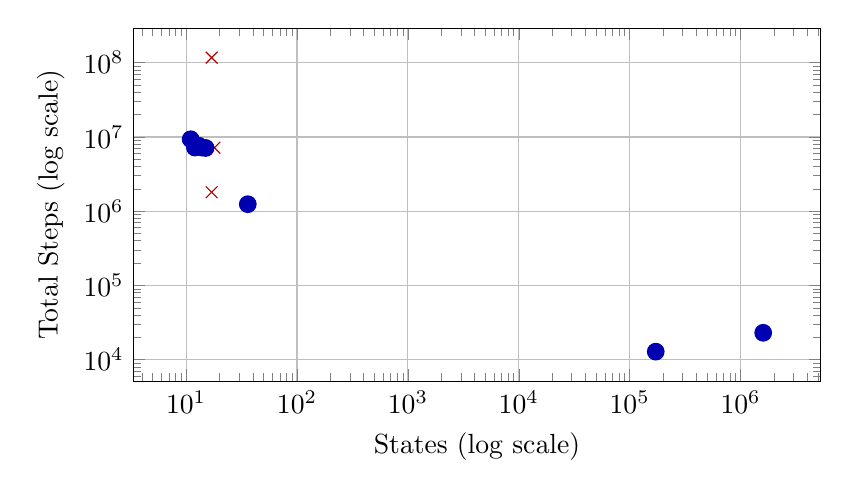
\begin{tikzpicture}
\begin{axis}[
  xlabel={States (log scale)},
  ylabel={Total Steps (log scale)},
  xmode=log, ymode=log,
  width=0.85\textwidth,
  height=0.5\textwidth,
  grid=major,
  nodes near coords,
  nodes near coords style={font=\tiny, anchor=south west},
  point meta=explicit symbolic,
  scatter/classes={
    pass={mark=*, blue!70!black, mark size=3pt},
    fail={mark=x, red!70!black, mark size=3pt}},
]
\addplot[scatter, only marks, scatter src=explicit symbolic] coordinates {
  (14, 7186258) [pass] %% A
  (13, 7584139) [pass] %% B
  (13, 7584139) [pass] %% C
  (17, 117093715) [fail] %% D
  (171847, 12824) [pass] %% E
  (11, 9319410) [pass] %% F
  (36, 1242622) [pass] %% G
  (12, 7204678) [pass] %% H
  (1600227, 23022) [pass] %% I
  (18, 7168851) [fail] %% J
  (17, 1800985) [fail] %% K
  (15, 7106650) [pass] %% L
};
\end{axis}
\end{tikzpicture}
\caption{Machine size (states) vs.\ total execution steps. Two distinct clusters emerge: compact hand-written machines (10--36 states) and precomputed lookup tables (100K+ states).}
\end{figure}

\subsection{Step Count Growth}

\begin{figure}[H]
\centering
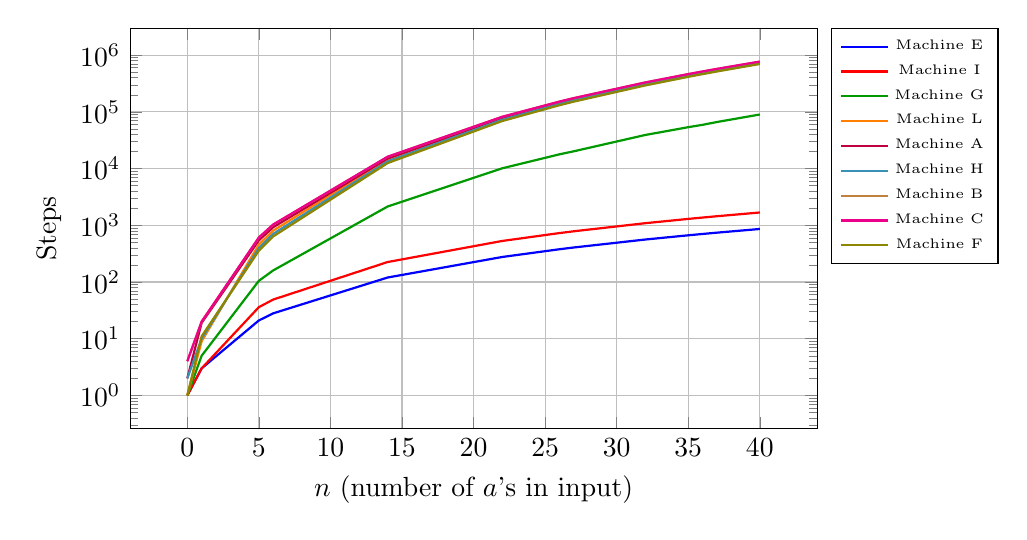
\begin{tikzpicture}
\begin{axis}[
  xlabel={$n$ (number of $a$'s in input)},
  ylabel={Steps},
  ymode=log,
  width=0.85\textwidth,
  height=0.55\textwidth,
  grid=major,
  legend style={at={(1.02,1)}, anchor=north west, font=\tiny},
  cycle list name=color list,
]
\addplot[blue, thick, mark=none] coordinates {
  (0, 1)
  (1, 3)
  (5, 21)
  (6, 28)
  (14, 120)
  (22, 276)
  (26, 378)
  (27, 406)
  (32, 561)
  (35, 666)
  (36, 703)
  (37, 741)
  (40, 861)
};
\addlegendentry{Machine E}
\addplot[red, thick, mark=none] coordinates {
  (0, 1)
  (1, 3)
  (5, 36)
  (6, 49)
  (14, 225)
  (22, 529)
  (26, 729)
  (27, 784)
  (32, 1089)
  (35, 1296)
  (36, 1369)
  (37, 1444)
  (40, 1681)
};
\addlegendentry{Machine I}
\addplot[green!60!black, thick, mark=none] coordinates {
  (0, 1)
  (1, 5)
  (5, 105)
  (6, 160)
  (14, 2146)
  (22, 10100)
  (26, 17828)
  (27, 20157)
  (32, 39132)
  (35, 53645)
  (36, 59054)
  (37, 66167)
  (40, 89838)
};
\addlegendentry{Machine G}
\addplot[orange, thick, mark=none] coordinates {
  (0, 1)
  (1, 9)
  (5, 457)
  (6, 804)
  (14, 14452)
  (22, 76260)
  (26, 142984)
  (27, 164940)
  (32, 314845)
  (35, 443692)
  (36, 494349)
  (37, 549225)
  (40, 741477)
};
\addlegendentry{Machine L}
\addplot[purple, thick, mark=none] coordinates {
  (0, 2)
  (1, 19)
  (5, 543)
  (6, 924)
  (14, 15060)
  (22, 77740)
  (26, 145044)
  (27, 167160)
  (32, 317955)
  (35, 447408)
  (36, 498279)
  (37, 553375)
  (40, 746323)
};
\addlegendentry{Machine A}
\addplot[cyan!70!black, thick, mark=none] coordinates {
  (0, 2)
  (1, 10)
  (5, 396)
  (6, 705)
  (14, 13413)
  (22, 72425)
  (26, 136735)
  (27, 157960)
  (32, 303345)
  (35, 428716)
  (36, 478075)
  (37, 531580)
  (40, 719261)
};
\addlegendentry{Machine H}
\addplot[brown, thick, mark=none] coordinates {
  (0, 4)
  (1, 20)
  (5, 608)
  (6, 1030)
  (14, 16166)
  (22, 81766)
  (26, 151570)
  (27, 174441)
  (32, 329891)
  (35, 462913)
  (36, 515115)
  (37, 571616)
  (40, 769243)
};
\addlegendentry{Machine B}
\addplot[magenta, thick, mark=none] coordinates {
  (0, 4)
  (1, 20)
  (5, 608)
  (6, 1030)
  (14, 16166)
  (22, 81766)
  (26, 151570)
  (27, 174441)
  (32, 329891)
  (35, 462913)
  (36, 515115)
  (37, 571616)
  (40, 769243)
};
\addlegendentry{Machine C}
\addplot[olive, thick, mark=none] coordinates {
  (0, 1)
  (1, 11)
  (5, 357)
  (6, 636)
  (14, 12504)
  (22, 68884)
  (26, 130886)
  (27, 151409)
  (32, 292434)
  (35, 414437)
  (36, 462536)
  (37, 514709)
  (40, 697942)
};
\addlegendentry{Machine F}
\end{axis}
\end{tikzpicture}
\caption{Steps vs.\ $n$ for correctly-accepted inputs. Precomputed machines show near-constant cost; hand-written machines show polynomial growth.}
\end{figure}

\subsection{Observations}

\textbf{Precomputed machines} (Machine E, Machine I) trade an enormous state space for minimal step counts. These machines effectively encode a lookup table, resolving each input in $O(n)$ steps or fewer.

\textbf{Hand-written machines} (Machine G, Machine L, Machine A, Machine H, Machine B, Machine C, Machine F) use compact representations (11--36 states) but require millions of steps on larger inputs. Machine G leads this group with 1,242,622 total steps, roughly 7$\times$ fewer than Machine F (9,319,410 total steps).

\textbf{Identical behavior:} Machine B and Machine C produced the exact same step count on every test case, suggesting functionally equivalent machines.

Machine D passed 30/41 test cases.
Machine J passed 22/41 test cases.
Machine K passed 40/41 test cases.

\section{Machine Details}

Each machine is shown with tape visualizations on small inputs. Highlighted cells indicate the head position.

\subsection*{Machine E}

\begin{tabular}{ll}
States & 171,847 \\
Transitions & 171,995 \\
Test cases passed & 41/41 \\
Average steps & 312 \\
Max steps (single case) & 861 \\
\end{tabular}
\medskip

\paragraph{Input: $\varepsilon$ (1 steps, Accept)}

\noindent
  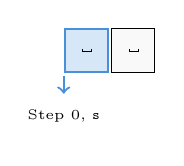
\begin{tikzpicture}
    \node[headcell] (c0) at (0.0, 0) {\textvisiblespace};
    \node[blankcell] (c1) at (0.6, 0) {\textvisiblespace};
    \draw[->, thick, headcell] (0.0, -0.32) -- (0.0, -0.55) node[below, font=\tiny] {Step 0, \texttt{s}};
  \end{tikzpicture}
\par\vspace{1mm}

\paragraph{Input: \texttt{ab} (3 steps, Accept)}

\noindent
  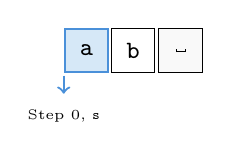
\begin{tikzpicture}
    \node[headcell] (c0) at (0.0, 0) {a};
    \node[cell] (c1) at (0.6, 0) {b};
    \node[blankcell] (c2) at (1.2, 0) {\textvisiblespace};
    \draw[->, thick, headcell] (0.0, -0.32) -- (0.0, -0.55) node[below, font=\tiny] {Step 0, \texttt{s}};
  \end{tikzpicture}
\par\vspace{1mm}
  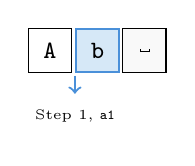
\begin{tikzpicture}
    \node[cell] (c0) at (0.0, 0) {A};
    \node[headcell] (c1) at (0.6, 0) {b};
    \node[blankcell] (c2) at (1.2, 0) {\textvisiblespace};
    \draw[->, thick, headcell] (0.6, -0.32) -- (0.6, -0.55) node[below, font=\tiny] {Step 1, \texttt{a1}};
  \end{tikzpicture}
\par\vspace{1mm}
  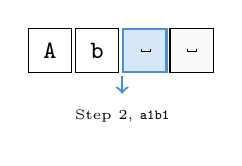
\begin{tikzpicture}
    \node[cell] (c0) at (0.0, 0) {A};
    \node[cell] (c1) at (0.6, 0) {b};
    \node[headcell] (c2) at (1.2, 0) {\textvisiblespace};
    \node[blankcell] (c3) at (1.8, 0) {\textvisiblespace};
    \draw[->, thick, headcell] (1.2, -0.32) -- (1.2, -0.55) node[below, font=\tiny] {Step 2, \texttt{a1b1}};
  \end{tikzpicture}
\par\vspace{1mm}

\paragraph{Input: \texttt{aabbbbbb} (6 steps, Reject)}

\noindent
  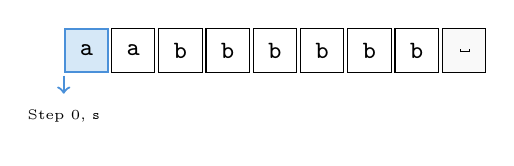
\begin{tikzpicture}
    \node[headcell] (c0) at (0.0, 0) {a};
    \node[cell] (c1) at (0.6, 0) {a};
    \node[cell] (c2) at (1.2, 0) {b};
    \node[cell] (c3) at (1.8, 0) {b};
    \node[cell] (c4) at (2.4, 0) {b};
    \node[cell] (c5) at (3.0, 0) {b};
    \node[cell] (c6) at (3.6, 0) {b};
    \node[cell] (c7) at (4.2, 0) {b};
    \node[blankcell] (c8) at (4.8, 0) {\textvisiblespace};
    \draw[->, thick, headcell] (0.0, -0.32) -- (0.0, -0.55) node[below, font=\tiny] {Step 0, \texttt{s}};
  \end{tikzpicture}
\par\vspace{1mm}
  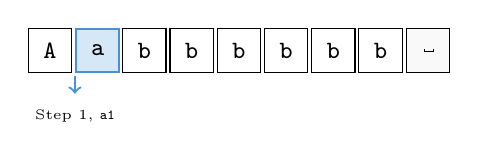
\begin{tikzpicture}
    \node[cell] (c0) at (0.0, 0) {A};
    \node[headcell] (c1) at (0.6, 0) {a};
    \node[cell] (c2) at (1.2, 0) {b};
    \node[cell] (c3) at (1.8, 0) {b};
    \node[cell] (c4) at (2.4, 0) {b};
    \node[cell] (c5) at (3.0, 0) {b};
    \node[cell] (c6) at (3.6, 0) {b};
    \node[cell] (c7) at (4.2, 0) {b};
    \node[blankcell] (c8) at (4.8, 0) {\textvisiblespace};
    \draw[->, thick, headcell] (0.6, -0.32) -- (0.6, -0.55) node[below, font=\tiny] {Step 1, \texttt{a1}};
  \end{tikzpicture}
\par\vspace{1mm}
  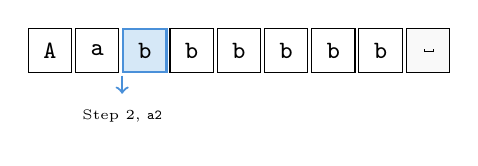
\begin{tikzpicture}
    \node[cell] (c0) at (0.0, 0) {A};
    \node[cell] (c1) at (0.6, 0) {a};
    \node[headcell] (c2) at (1.2, 0) {b};
    \node[cell] (c3) at (1.8, 0) {b};
    \node[cell] (c4) at (2.4, 0) {b};
    \node[cell] (c5) at (3.0, 0) {b};
    \node[cell] (c6) at (3.6, 0) {b};
    \node[cell] (c7) at (4.2, 0) {b};
    \node[blankcell] (c8) at (4.8, 0) {\textvisiblespace};
    \draw[->, thick, headcell] (1.2, -0.32) -- (1.2, -0.55) node[below, font=\tiny] {Step 2, \texttt{a2}};
  \end{tikzpicture}
\par\vspace{1mm}
  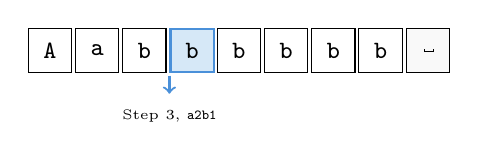
\begin{tikzpicture}
    \node[cell] (c0) at (0.0, 0) {A};
    \node[cell] (c1) at (0.6, 0) {a};
    \node[cell] (c2) at (1.2, 0) {b};
    \node[headcell] (c3) at (1.8, 0) {b};
    \node[cell] (c4) at (2.4, 0) {b};
    \node[cell] (c5) at (3.0, 0) {b};
    \node[cell] (c6) at (3.6, 0) {b};
    \node[cell] (c7) at (4.2, 0) {b};
    \node[blankcell] (c8) at (4.8, 0) {\textvisiblespace};
    \draw[->, thick, headcell] (1.8, -0.32) -- (1.8, -0.55) node[below, font=\tiny] {Step 3, \texttt{a2b1}};
  \end{tikzpicture}
\par\vspace{1mm}
  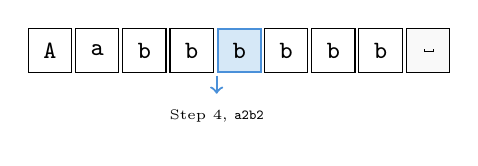
\begin{tikzpicture}
    \node[cell] (c0) at (0.0, 0) {A};
    \node[cell] (c1) at (0.6, 0) {a};
    \node[cell] (c2) at (1.2, 0) {b};
    \node[cell] (c3) at (1.8, 0) {b};
    \node[headcell] (c4) at (2.4, 0) {b};
    \node[cell] (c5) at (3.0, 0) {b};
    \node[cell] (c6) at (3.6, 0) {b};
    \node[cell] (c7) at (4.2, 0) {b};
    \node[blankcell] (c8) at (4.8, 0) {\textvisiblespace};
    \draw[->, thick, headcell] (2.4, -0.32) -- (2.4, -0.55) node[below, font=\tiny] {Step 4, \texttt{a2b2}};
  \end{tikzpicture}
\par\vspace{1mm}
  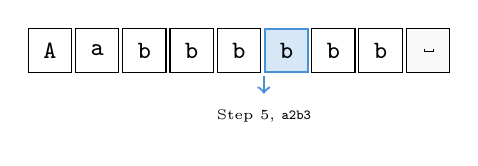
\begin{tikzpicture}
    \node[cell] (c0) at (0.0, 0) {A};
    \node[cell] (c1) at (0.6, 0) {a};
    \node[cell] (c2) at (1.2, 0) {b};
    \node[cell] (c3) at (1.8, 0) {b};
    \node[cell] (c4) at (2.4, 0) {b};
    \node[headcell] (c5) at (3.0, 0) {b};
    \node[cell] (c6) at (3.6, 0) {b};
    \node[cell] (c7) at (4.2, 0) {b};
    \node[blankcell] (c8) at (4.8, 0) {\textvisiblespace};
    \draw[->, thick, headcell] (3.0, -0.32) -- (3.0, -0.55) node[below, font=\tiny] {Step 5, \texttt{a2b3}};
  \end{tikzpicture}
\par\vspace{1mm}

\clearpage
\subsection*{Machine I}

\begin{tabular}{ll}
States & 1,600,227 \\
Transitions & 1,611,613 \\
Test cases passed & 41/41 \\
Average steps & 561 \\
Max steps (single case) & 1,681 \\
\end{tabular}
\medskip

\paragraph{Input: $\varepsilon$ (1 steps, Accept)}

\noindent
  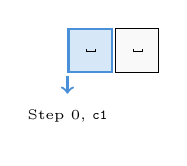
\begin{tikzpicture}
    \node[headcell] (c0) at (0.0, 0) {\textvisiblespace};
    \node[blankcell] (c1) at (0.6, 0) {\textvisiblespace};
    \draw[->, thick, headcell] (0.0, -0.32) -- (0.0, -0.55) node[below, font=\tiny] {Step 0, \texttt{c1}};
  \end{tikzpicture}
\par\vspace{1mm}

\paragraph{Input: \texttt{ab} (3 steps, Accept)}

\noindent
  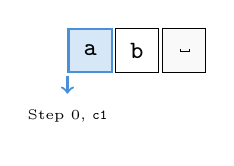
\begin{tikzpicture}
    \node[headcell] (c0) at (0.0, 0) {a};
    \node[cell] (c1) at (0.6, 0) {b};
    \node[blankcell] (c2) at (1.2, 0) {\textvisiblespace};
    \draw[->, thick, headcell] (0.0, -0.32) -- (0.0, -0.55) node[below, font=\tiny] {Step 0, \texttt{c1}};
  \end{tikzpicture}
\par\vspace{1mm}
  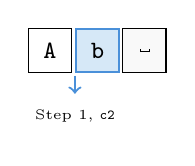
\begin{tikzpicture}
    \node[cell] (c0) at (0.0, 0) {A};
    \node[headcell] (c1) at (0.6, 0) {b};
    \node[blankcell] (c2) at (1.2, 0) {\textvisiblespace};
    \draw[->, thick, headcell] (0.6, -0.32) -- (0.6, -0.55) node[below, font=\tiny] {Step 1, \texttt{c2}};
  \end{tikzpicture}
\par\vspace{1mm}
  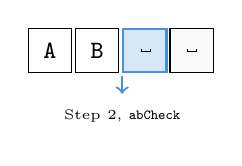
\begin{tikzpicture}
    \node[cell] (c0) at (0.0, 0) {A};
    \node[cell] (c1) at (0.6, 0) {B};
    \node[headcell] (c2) at (1.2, 0) {\textvisiblespace};
    \node[blankcell] (c3) at (1.8, 0) {\textvisiblespace};
    \draw[->, thick, headcell] (1.2, -0.32) -- (1.2, -0.55) node[below, font=\tiny] {Step 2, \texttt{abCheck}};
  \end{tikzpicture}
\par\vspace{1mm}

\paragraph{Input: \texttt{aabbbbbb} (11 steps, Reject)}

\noindent
  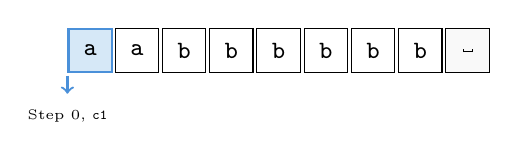
\begin{tikzpicture}
    \node[headcell] (c0) at (0.0, 0) {a};
    \node[cell] (c1) at (0.6, 0) {a};
    \node[cell] (c2) at (1.2, 0) {b};
    \node[cell] (c3) at (1.8, 0) {b};
    \node[cell] (c4) at (2.4, 0) {b};
    \node[cell] (c5) at (3.0, 0) {b};
    \node[cell] (c6) at (3.6, 0) {b};
    \node[cell] (c7) at (4.2, 0) {b};
    \node[blankcell] (c8) at (4.8, 0) {\textvisiblespace};
    \draw[->, thick, headcell] (0.0, -0.32) -- (0.0, -0.55) node[below, font=\tiny] {Step 0, \texttt{c1}};
  \end{tikzpicture}
\par\vspace{1mm}
  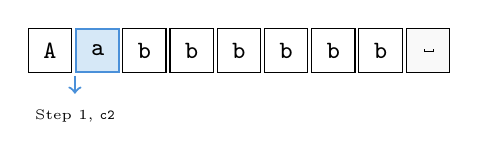
\begin{tikzpicture}
    \node[cell] (c0) at (0.0, 0) {A};
    \node[headcell] (c1) at (0.6, 0) {a};
    \node[cell] (c2) at (1.2, 0) {b};
    \node[cell] (c3) at (1.8, 0) {b};
    \node[cell] (c4) at (2.4, 0) {b};
    \node[cell] (c5) at (3.0, 0) {b};
    \node[cell] (c6) at (3.6, 0) {b};
    \node[cell] (c7) at (4.2, 0) {b};
    \node[blankcell] (c8) at (4.8, 0) {\textvisiblespace};
    \draw[->, thick, headcell] (0.6, -0.32) -- (0.6, -0.55) node[below, font=\tiny] {Step 1, \texttt{c2}};
  \end{tikzpicture}
\par\vspace{1mm}
  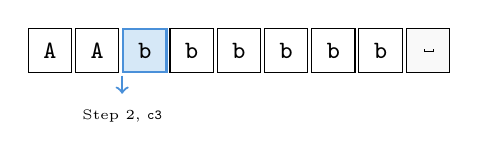
\begin{tikzpicture}
    \node[cell] (c0) at (0.0, 0) {A};
    \node[cell] (c1) at (0.6, 0) {A};
    \node[headcell] (c2) at (1.2, 0) {b};
    \node[cell] (c3) at (1.8, 0) {b};
    \node[cell] (c4) at (2.4, 0) {b};
    \node[cell] (c5) at (3.0, 0) {b};
    \node[cell] (c6) at (3.6, 0) {b};
    \node[cell] (c7) at (4.2, 0) {b};
    \node[blankcell] (c8) at (4.8, 0) {\textvisiblespace};
    \draw[->, thick, headcell] (1.2, -0.32) -- (1.2, -0.55) node[below, font=\tiny] {Step 2, \texttt{c3}};
  \end{tikzpicture}
\par\vspace{1mm}
  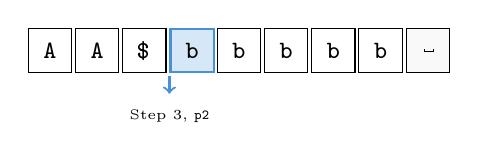
\begin{tikzpicture}
    \node[cell] (c0) at (0.0, 0) {A};
    \node[cell] (c1) at (0.6, 0) {A};
    \node[cell] (c2) at (1.2, 0) {\$};
    \node[headcell] (c3) at (1.8, 0) {b};
    \node[cell] (c4) at (2.4, 0) {b};
    \node[cell] (c5) at (3.0, 0) {b};
    \node[cell] (c6) at (3.6, 0) {b};
    \node[cell] (c7) at (4.2, 0) {b};
    \node[blankcell] (c8) at (4.8, 0) {\textvisiblespace};
    \draw[->, thick, headcell] (1.8, -0.32) -- (1.8, -0.55) node[below, font=\tiny] {Step 3, \texttt{p2}};
  \end{tikzpicture}
\par\vspace{1mm}
  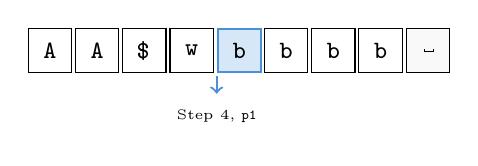
\begin{tikzpicture}
    \node[cell] (c0) at (0.0, 0) {A};
    \node[cell] (c1) at (0.6, 0) {A};
    \node[cell] (c2) at (1.2, 0) {\$};
    \node[cell] (c3) at (1.8, 0) {w};
    \node[headcell] (c4) at (2.4, 0) {b};
    \node[cell] (c5) at (3.0, 0) {b};
    \node[cell] (c6) at (3.6, 0) {b};
    \node[cell] (c7) at (4.2, 0) {b};
    \node[blankcell] (c8) at (4.8, 0) {\textvisiblespace};
    \draw[->, thick, headcell] (2.4, -0.32) -- (2.4, -0.55) node[below, font=\tiny] {Step 4, \texttt{p1}};
  \end{tikzpicture}
\par\vspace{1mm}
  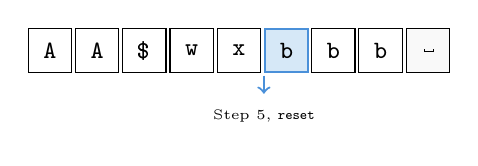
\begin{tikzpicture}
    \node[cell] (c0) at (0.0, 0) {A};
    \node[cell] (c1) at (0.6, 0) {A};
    \node[cell] (c2) at (1.2, 0) {\$};
    \node[cell] (c3) at (1.8, 0) {w};
    \node[cell] (c4) at (2.4, 0) {x};
    \node[headcell] (c5) at (3.0, 0) {b};
    \node[cell] (c6) at (3.6, 0) {b};
    \node[cell] (c7) at (4.2, 0) {b};
    \node[blankcell] (c8) at (4.8, 0) {\textvisiblespace};
    \draw[->, thick, headcell] (3.0, -0.32) -- (3.0, -0.55) node[below, font=\tiny] {Step 5, \texttt{reset}};
  \end{tikzpicture}
\par\vspace{1mm}
  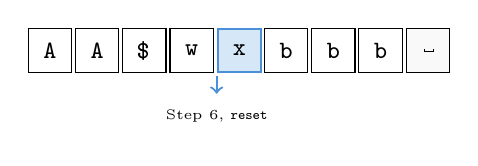
\begin{tikzpicture}
    \node[cell] (c0) at (0.0, 0) {A};
    \node[cell] (c1) at (0.6, 0) {A};
    \node[cell] (c2) at (1.2, 0) {\$};
    \node[cell] (c3) at (1.8, 0) {w};
    \node[headcell] (c4) at (2.4, 0) {x};
    \node[cell] (c5) at (3.0, 0) {b};
    \node[cell] (c6) at (3.6, 0) {b};
    \node[cell] (c7) at (4.2, 0) {b};
    \node[blankcell] (c8) at (4.8, 0) {\textvisiblespace};
    \draw[->, thick, headcell] (2.4, -0.32) -- (2.4, -0.55) node[below, font=\tiny] {Step 6, \texttt{reset}};
  \end{tikzpicture}
\par\vspace{1mm}
  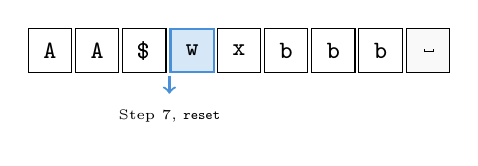
\begin{tikzpicture}
    \node[cell] (c0) at (0.0, 0) {A};
    \node[cell] (c1) at (0.6, 0) {A};
    \node[cell] (c2) at (1.2, 0) {\$};
    \node[headcell] (c3) at (1.8, 0) {w};
    \node[cell] (c4) at (2.4, 0) {x};
    \node[cell] (c5) at (3.0, 0) {b};
    \node[cell] (c6) at (3.6, 0) {b};
    \node[cell] (c7) at (4.2, 0) {b};
    \node[blankcell] (c8) at (4.8, 0) {\textvisiblespace};
    \draw[->, thick, headcell] (1.8, -0.32) -- (1.8, -0.55) node[below, font=\tiny] {Step 7, \texttt{reset}};
  \end{tikzpicture}
\par\vspace{1mm}
  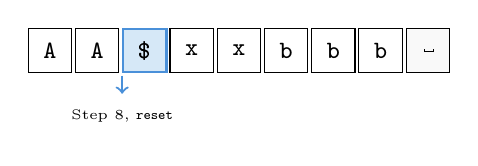
\begin{tikzpicture}
    \node[cell] (c0) at (0.0, 0) {A};
    \node[cell] (c1) at (0.6, 0) {A};
    \node[headcell] (c2) at (1.2, 0) {\$};
    \node[cell] (c3) at (1.8, 0) {x};
    \node[cell] (c4) at (2.4, 0) {x};
    \node[cell] (c5) at (3.0, 0) {b};
    \node[cell] (c6) at (3.6, 0) {b};
    \node[cell] (c7) at (4.2, 0) {b};
    \node[blankcell] (c8) at (4.8, 0) {\textvisiblespace};
    \draw[->, thick, headcell] (1.2, -0.32) -- (1.2, -0.55) node[below, font=\tiny] {Step 8, \texttt{reset}};
  \end{tikzpicture}
\par\vspace{1mm}
  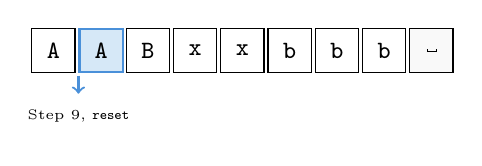
\begin{tikzpicture}
    \node[cell] (c0) at (0.0, 0) {A};
    \node[headcell] (c1) at (0.6, 0) {A};
    \node[cell] (c2) at (1.2, 0) {B};
    \node[cell] (c3) at (1.8, 0) {x};
    \node[cell] (c4) at (2.4, 0) {x};
    \node[cell] (c5) at (3.0, 0) {b};
    \node[cell] (c6) at (3.6, 0) {b};
    \node[cell] (c7) at (4.2, 0) {b};
    \node[blankcell] (c8) at (4.8, 0) {\textvisiblespace};
    \draw[->, thick, headcell] (0.6, -0.32) -- (0.6, -0.55) node[below, font=\tiny] {Step 9, \texttt{reset}};
  \end{tikzpicture}
\par\vspace{1mm}
  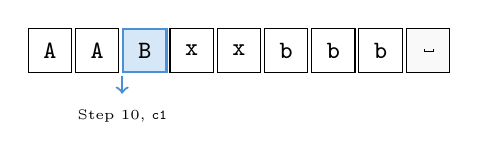
\begin{tikzpicture}
    \node[cell] (c0) at (0.0, 0) {A};
    \node[cell] (c1) at (0.6, 0) {A};
    \node[headcell] (c2) at (1.2, 0) {B};
    \node[cell] (c3) at (1.8, 0) {x};
    \node[cell] (c4) at (2.4, 0) {x};
    \node[cell] (c5) at (3.0, 0) {b};
    \node[cell] (c6) at (3.6, 0) {b};
    \node[cell] (c7) at (4.2, 0) {b};
    \node[blankcell] (c8) at (4.8, 0) {\textvisiblespace};
    \draw[->, thick, headcell] (1.2, -0.32) -- (1.2, -0.55) node[below, font=\tiny] {Step 10, \texttt{c1}};
  \end{tikzpicture}
\par\vspace{1mm}

\clearpage
\subsection*{Machine G}

\begin{tabular}{ll}
States & 36 \\
Transitions & 105 \\
Test cases passed & 41/41 \\
Average steps & 30,307 \\
Max steps (single case) & 226,240 \\
\end{tabular}
\medskip

\paragraph{Input: $\varepsilon$ (1 steps, Accept)}

\noindent
  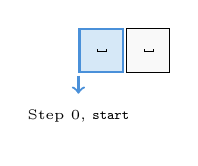
\begin{tikzpicture}
    \node[headcell] (c0) at (0.0, 0) {\textvisiblespace};
    \node[blankcell] (c1) at (0.6, 0) {\textvisiblespace};
    \draw[->, thick, headcell] (0.0, -0.32) -- (0.0, -0.55) node[below, font=\tiny] {Step 0, \texttt{start}};
  \end{tikzpicture}
\par\vspace{1mm}

\paragraph{Input: \texttt{ab} (5 steps, Accept)}

\noindent
  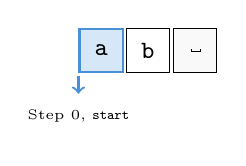
\begin{tikzpicture}
    \node[headcell] (c0) at (0.0, 0) {a};
    \node[cell] (c1) at (0.6, 0) {b};
    \node[blankcell] (c2) at (1.2, 0) {\textvisiblespace};
    \draw[->, thick, headcell] (0.0, -0.32) -- (0.0, -0.55) node[below, font=\tiny] {Step 0, \texttt{start}};
  \end{tikzpicture}
\par\vspace{1mm}
  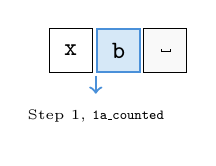
\begin{tikzpicture}
    \node[cell] (c0) at (0.0, 0) {x};
    \node[headcell] (c1) at (0.6, 0) {b};
    \node[blankcell] (c2) at (1.2, 0) {\textvisiblespace};
    \draw[->, thick, headcell] (0.6, -0.32) -- (0.6, -0.55) node[below, font=\tiny] {Step 1, \texttt{1a\_counted}};
  \end{tikzpicture}
\par\vspace{1mm}
  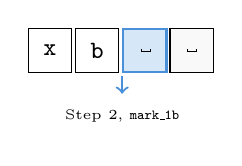
\begin{tikzpicture}
    \node[cell] (c0) at (0.0, 0) {x};
    \node[cell] (c1) at (0.6, 0) {b};
    \node[headcell] (c2) at (1.2, 0) {\textvisiblespace};
    \node[blankcell] (c3) at (1.8, 0) {\textvisiblespace};
    \draw[->, thick, headcell] (1.2, -0.32) -- (1.2, -0.55) node[below, font=\tiny] {Step 2, \texttt{mark\_1b}};
  \end{tikzpicture}
\par\vspace{1mm}
  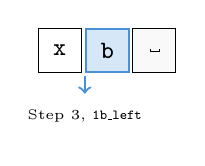
\begin{tikzpicture}
    \node[cell] (c0) at (0.0, 0) {x};
    \node[headcell] (c1) at (0.6, 0) {b};
    \node[blankcell] (c2) at (1.2, 0) {\textvisiblespace};
    \draw[->, thick, headcell] (0.6, -0.32) -- (0.6, -0.55) node[below, font=\tiny] {Step 3, \texttt{1b\_left}};
  \end{tikzpicture}
\par\vspace{1mm}
  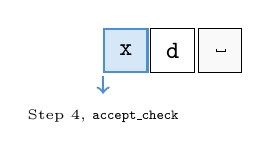
\begin{tikzpicture}
    \node[headcell] (c0) at (0.0, 0) {x};
    \node[cell] (c1) at (0.6, 0) {d};
    \node[blankcell] (c2) at (1.2, 0) {\textvisiblespace};
    \draw[->, thick, headcell] (0.0, -0.32) -- (0.0, -0.55) node[below, font=\tiny] {Step 4, \texttt{accept\_check}};
  \end{tikzpicture}
\par\vspace{1mm}

\paragraph{Input: \texttt{aabbbbbb} (29 steps, Reject)}

\noindent
  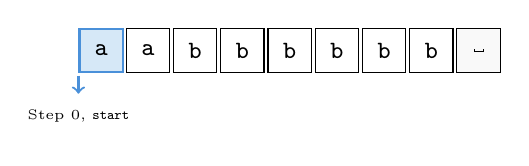
\begin{tikzpicture}
    \node[headcell] (c0) at (0.0, 0) {a};
    \node[cell] (c1) at (0.6, 0) {a};
    \node[cell] (c2) at (1.2, 0) {b};
    \node[cell] (c3) at (1.8, 0) {b};
    \node[cell] (c4) at (2.4, 0) {b};
    \node[cell] (c5) at (3.0, 0) {b};
    \node[cell] (c6) at (3.6, 0) {b};
    \node[cell] (c7) at (4.2, 0) {b};
    \node[blankcell] (c8) at (4.8, 0) {\textvisiblespace};
    \draw[->, thick, headcell] (0.0, -0.32) -- (0.0, -0.55) node[below, font=\tiny] {Step 0, \texttt{start}};
  \end{tikzpicture}
\par\vspace{1mm}
  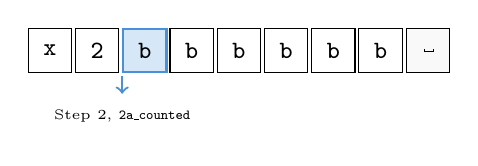
\begin{tikzpicture}
    \node[cell] (c0) at (0.0, 0) {x};
    \node[cell] (c1) at (0.6, 0) {2};
    \node[headcell] (c2) at (1.2, 0) {b};
    \node[cell] (c3) at (1.8, 0) {b};
    \node[cell] (c4) at (2.4, 0) {b};
    \node[cell] (c5) at (3.0, 0) {b};
    \node[cell] (c6) at (3.6, 0) {b};
    \node[cell] (c7) at (4.2, 0) {b};
    \node[blankcell] (c8) at (4.8, 0) {\textvisiblespace};
    \draw[->, thick, headcell] (1.2, -0.32) -- (1.2, -0.55) node[below, font=\tiny] {Step 2, \texttt{2a\_counted}};
  \end{tikzpicture}
\par\vspace{1mm}
  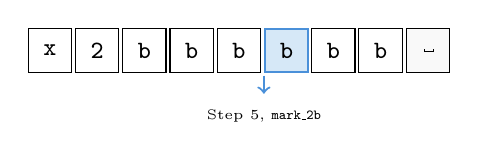
\begin{tikzpicture}
    \node[cell] (c0) at (0.0, 0) {x};
    \node[cell] (c1) at (0.6, 0) {2};
    \node[cell] (c2) at (1.2, 0) {b};
    \node[cell] (c3) at (1.8, 0) {b};
    \node[cell] (c4) at (2.4, 0) {b};
    \node[headcell] (c5) at (3.0, 0) {b};
    \node[cell] (c6) at (3.6, 0) {b};
    \node[cell] (c7) at (4.2, 0) {b};
    \node[blankcell] (c8) at (4.8, 0) {\textvisiblespace};
    \draw[->, thick, headcell] (3.0, -0.32) -- (3.0, -0.55) node[below, font=\tiny] {Step 5, \texttt{mark\_2b}};
  \end{tikzpicture}
\par\vspace{1mm}
  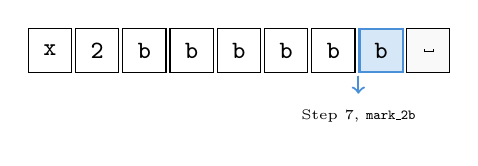
\begin{tikzpicture}
    \node[cell] (c0) at (0.0, 0) {x};
    \node[cell] (c1) at (0.6, 0) {2};
    \node[cell] (c2) at (1.2, 0) {b};
    \node[cell] (c3) at (1.8, 0) {b};
    \node[cell] (c4) at (2.4, 0) {b};
    \node[cell] (c5) at (3.0, 0) {b};
    \node[cell] (c6) at (3.6, 0) {b};
    \node[headcell] (c7) at (4.2, 0) {b};
    \node[blankcell] (c8) at (4.8, 0) {\textvisiblespace};
    \draw[->, thick, headcell] (4.2, -0.32) -- (4.2, -0.55) node[below, font=\tiny] {Step 7, \texttt{mark\_2b}};
  \end{tikzpicture}
\par\vspace{1mm}
  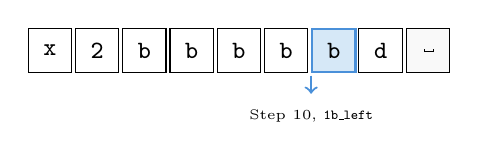
\begin{tikzpicture}
    \node[cell] (c0) at (0.0, 0) {x};
    \node[cell] (c1) at (0.6, 0) {2};
    \node[cell] (c2) at (1.2, 0) {b};
    \node[cell] (c3) at (1.8, 0) {b};
    \node[cell] (c4) at (2.4, 0) {b};
    \node[cell] (c5) at (3.0, 0) {b};
    \node[headcell] (c6) at (3.6, 0) {b};
    \node[cell] (c7) at (4.2, 0) {d};
    \node[blankcell] (c8) at (4.8, 0) {\textvisiblespace};
    \draw[->, thick, headcell] (3.6, -0.32) -- (3.6, -0.55) node[below, font=\tiny] {Step 10, \texttt{1b\_left}};
  \end{tikzpicture}
\par\vspace{1mm}
  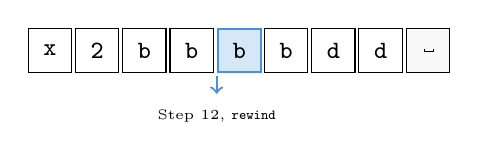
\begin{tikzpicture}
    \node[cell] (c0) at (0.0, 0) {x};
    \node[cell] (c1) at (0.6, 0) {2};
    \node[cell] (c2) at (1.2, 0) {b};
    \node[cell] (c3) at (1.8, 0) {b};
    \node[headcell] (c4) at (2.4, 0) {b};
    \node[cell] (c5) at (3.0, 0) {b};
    \node[cell] (c6) at (3.6, 0) {d};
    \node[cell] (c7) at (4.2, 0) {d};
    \node[blankcell] (c8) at (4.8, 0) {\textvisiblespace};
    \draw[->, thick, headcell] (2.4, -0.32) -- (2.4, -0.55) node[below, font=\tiny] {Step 12, \texttt{rewind}};
  \end{tikzpicture}
\par\vspace{1mm}
  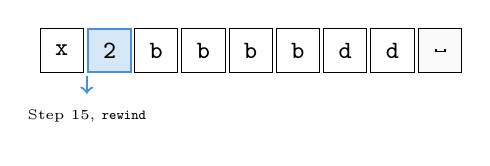
\begin{tikzpicture}
    \node[cell] (c0) at (0.0, 0) {x};
    \node[headcell] (c1) at (0.6, 0) {2};
    \node[cell] (c2) at (1.2, 0) {b};
    \node[cell] (c3) at (1.8, 0) {b};
    \node[cell] (c4) at (2.4, 0) {b};
    \node[cell] (c5) at (3.0, 0) {b};
    \node[cell] (c6) at (3.6, 0) {d};
    \node[cell] (c7) at (4.2, 0) {d};
    \node[blankcell] (c8) at (4.8, 0) {\textvisiblespace};
    \draw[->, thick, headcell] (0.6, -0.32) -- (0.6, -0.55) node[below, font=\tiny] {Step 15, \texttt{rewind}};
  \end{tikzpicture}
\par\vspace{1mm}
  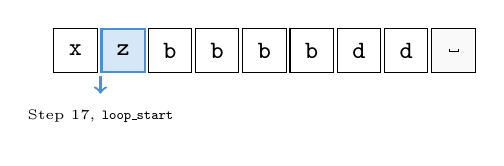
\begin{tikzpicture}
    \node[cell] (c0) at (0.0, 0) {x};
    \node[headcell] (c1) at (0.6, 0) {z};
    \node[cell] (c2) at (1.2, 0) {b};
    \node[cell] (c3) at (1.8, 0) {b};
    \node[cell] (c4) at (2.4, 0) {b};
    \node[cell] (c5) at (3.0, 0) {b};
    \node[cell] (c6) at (3.6, 0) {d};
    \node[cell] (c7) at (4.2, 0) {d};
    \node[blankcell] (c8) at (4.8, 0) {\textvisiblespace};
    \draw[->, thick, headcell] (0.6, -0.32) -- (0.6, -0.55) node[below, font=\tiny] {Step 17, \texttt{loop\_start}};
  \end{tikzpicture}
\par\vspace{1mm}
  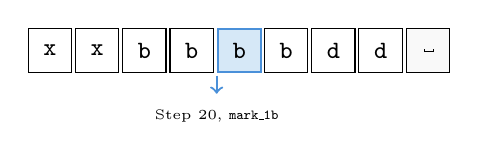
\begin{tikzpicture}
    \node[cell] (c0) at (0.0, 0) {x};
    \node[cell] (c1) at (0.6, 0) {x};
    \node[cell] (c2) at (1.2, 0) {b};
    \node[cell] (c3) at (1.8, 0) {b};
    \node[headcell] (c4) at (2.4, 0) {b};
    \node[cell] (c5) at (3.0, 0) {b};
    \node[cell] (c6) at (3.6, 0) {d};
    \node[cell] (c7) at (4.2, 0) {d};
    \node[blankcell] (c8) at (4.8, 0) {\textvisiblespace};
    \draw[->, thick, headcell] (2.4, -0.32) -- (2.4, -0.55) node[below, font=\tiny] {Step 20, \texttt{mark\_1b}};
  \end{tikzpicture}
\par\vspace{1mm}
  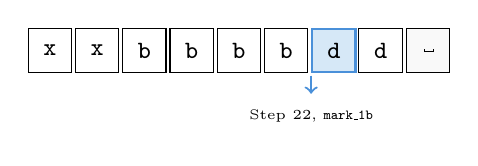
\begin{tikzpicture}
    \node[cell] (c0) at (0.0, 0) {x};
    \node[cell] (c1) at (0.6, 0) {x};
    \node[cell] (c2) at (1.2, 0) {b};
    \node[cell] (c3) at (1.8, 0) {b};
    \node[cell] (c4) at (2.4, 0) {b};
    \node[cell] (c5) at (3.0, 0) {b};
    \node[headcell] (c6) at (3.6, 0) {d};
    \node[cell] (c7) at (4.2, 0) {d};
    \node[blankcell] (c8) at (4.8, 0) {\textvisiblespace};
    \draw[->, thick, headcell] (3.6, -0.32) -- (3.6, -0.55) node[below, font=\tiny] {Step 22, \texttt{mark\_1b}};
  \end{tikzpicture}
\par\vspace{1mm}
  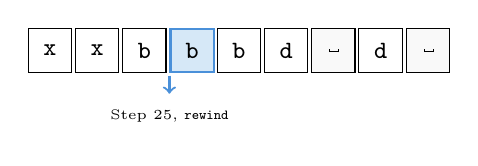
\begin{tikzpicture}
    \node[cell] (c0) at (0.0, 0) {x};
    \node[cell] (c1) at (0.6, 0) {x};
    \node[cell] (c2) at (1.2, 0) {b};
    \node[headcell] (c3) at (1.8, 0) {b};
    \node[cell] (c4) at (2.4, 0) {b};
    \node[cell] (c5) at (3.0, 0) {d};
    \node[blankcell] (c6) at (3.6, 0) {\textvisiblespace};
    \node[cell] (c7) at (4.2, 0) {d};
    \node[blankcell] (c8) at (4.8, 0) {\textvisiblespace};
    \draw[->, thick, headcell] (1.8, -0.32) -- (1.8, -0.55) node[below, font=\tiny] {Step 25, \texttt{rewind}};
  \end{tikzpicture}
\par\vspace{1mm}
  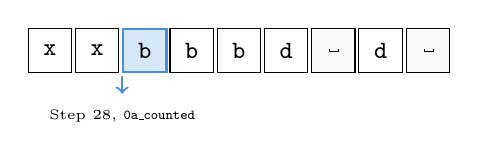
\begin{tikzpicture}
    \node[cell] (c0) at (0.0, 0) {x};
    \node[cell] (c1) at (0.6, 0) {x};
    \node[headcell] (c2) at (1.2, 0) {b};
    \node[cell] (c3) at (1.8, 0) {b};
    \node[cell] (c4) at (2.4, 0) {b};
    \node[cell] (c5) at (3.0, 0) {d};
    \node[blankcell] (c6) at (3.6, 0) {\textvisiblespace};
    \node[cell] (c7) at (4.2, 0) {d};
    \node[blankcell] (c8) at (4.8, 0) {\textvisiblespace};
    \draw[->, thick, headcell] (1.2, -0.32) -- (1.2, -0.55) node[below, font=\tiny] {Step 28, \texttt{0a\_counted}};
  \end{tikzpicture}
\par\vspace{1mm}

\clearpage
\subsection*{Machine L}

\begin{tabular}{ll}
States & 15 \\
Transitions & 104 \\
Test cases passed & 41/41 \\
Average steps & 173,332 \\
Max steps (single case) & 741,477 \\
\end{tabular}
\medskip

\paragraph{Input: $\varepsilon$ (1 steps, Accept)}

\noindent
  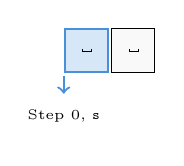
\begin{tikzpicture}
    \node[headcell] (c0) at (0.0, 0) {\textvisiblespace};
    \node[blankcell] (c1) at (0.6, 0) {\textvisiblespace};
    \draw[->, thick, headcell] (0.0, -0.32) -- (0.0, -0.55) node[below, font=\tiny] {Step 0, \texttt{s}};
  \end{tikzpicture}
\par\vspace{1mm}

\paragraph{Input: \texttt{ab} (9 steps, Accept)}

\noindent
  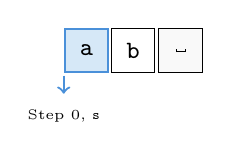
\begin{tikzpicture}
    \node[headcell] (c0) at (0.0, 0) {a};
    \node[cell] (c1) at (0.6, 0) {b};
    \node[blankcell] (c2) at (1.2, 0) {\textvisiblespace};
    \draw[->, thick, headcell] (0.0, -0.32) -- (0.0, -0.55) node[below, font=\tiny] {Step 0, \texttt{s}};
  \end{tikzpicture}
\par\vspace{1mm}
  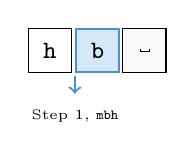
\begin{tikzpicture}
    \node[cell] (c0) at (0.0, 0) {h};
    \node[headcell] (c1) at (0.6, 0) {b};
    \node[blankcell] (c2) at (1.2, 0) {\textvisiblespace};
    \draw[->, thick, headcell] (0.6, -0.32) -- (0.6, -0.55) node[below, font=\tiny] {Step 1, \texttt{mbh}};
  \end{tikzpicture}
\par\vspace{1mm}
  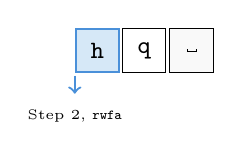
\begin{tikzpicture}
    \node[headcell] (c0) at (0.0, 0) {h};
    \node[cell] (c1) at (0.6, 0) {q};
    \node[blankcell] (c2) at (1.2, 0) {\textvisiblespace};
    \draw[->, thick, headcell] (0.0, -0.32) -- (0.0, -0.55) node[below, font=\tiny] {Step 2, \texttt{rwfa}};
  \end{tikzpicture}
\par\vspace{1mm}
  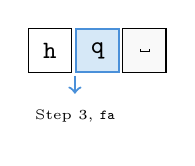
\begin{tikzpicture}
    \node[cell] (c0) at (0.0, 0) {h};
    \node[headcell] (c1) at (0.6, 0) {q};
    \node[blankcell] (c2) at (1.2, 0) {\textvisiblespace};
    \draw[->, thick, headcell] (0.6, -0.32) -- (0.6, -0.55) node[below, font=\tiny] {Step 3, \texttt{fa}};
  \end{tikzpicture}
\par\vspace{1mm}
  \begin{tikzpicture}
    \node[cell] (c0) at (0.0, 0) {h};
    \node[cell] (c1) at (0.6, 0) {q};
    \node[headcell] (c2) at (1.2, 0) {\textvisiblespace};
    \node[blankcell] (c3) at (1.8, 0) {\textvisiblespace};
    \draw[->, thick, headcell] (1.2, -0.32) -- (1.2, -0.55) node[below, font=\tiny] {Step 4, \texttt{fa}};
  \end{tikzpicture}
\par\vspace{1mm}
  \begin{tikzpicture}
    \node[cell] (c0) at (0.0, 0) {h};
    \node[headcell] (c1) at (0.6, 0) {q};
    \node[blankcell] (c2) at (1.2, 0) {\textvisiblespace};
    \draw[->, thick, headcell] (0.6, -0.32) -- (0.6, -0.55) node[below, font=\tiny] {Step 5, \texttt{fcr}};
  \end{tikzpicture}
\par\vspace{1mm}
  \begin{tikzpicture}
    \node[headcell] (c0) at (0.0, 0) {h};
    \node[cell] (c1) at (0.6, 0) {q};
    \node[blankcell] (c2) at (1.2, 0) {\textvisiblespace};
    \draw[->, thick, headcell] (0.0, -0.32) -- (0.0, -0.55) node[below, font=\tiny] {Step 6, \texttt{fcr}};
  \end{tikzpicture}
\par\vspace{1mm}
  \begin{tikzpicture}
    \node[cell] (c0) at (0.0, 0) {h};
    \node[headcell] (c1) at (0.6, 0) {q};
    \node[blankcell] (c2) at (1.2, 0) {\textvisiblespace};
    \draw[->, thick, headcell] (0.6, -0.32) -- (0.6, -0.55) node[below, font=\tiny] {Step 7, \texttt{fc}};
  \end{tikzpicture}
\par\vspace{1mm}
  \begin{tikzpicture}
    \node[cell] (c0) at (0.0, 0) {h};
    \node[cell] (c1) at (0.6, 0) {q};
    \node[headcell] (c2) at (1.2, 0) {\textvisiblespace};
    \node[blankcell] (c3) at (1.8, 0) {\textvisiblespace};
    \draw[->, thick, headcell] (1.2, -0.32) -- (1.2, -0.55) node[below, font=\tiny] {Step 8, \texttt{fc}};
  \end{tikzpicture}
\par\vspace{1mm}

\paragraph{Input: \texttt{aabbbbbb} (40 steps, Reject)}

\noindent
  \begin{tikzpicture}
    \node[headcell] (c0) at (0.0, 0) {a};
    \node[cell] (c1) at (0.6, 0) {a};
    \node[cell] (c2) at (1.2, 0) {b};
    \node[cell] (c3) at (1.8, 0) {b};
    \node[cell] (c4) at (2.4, 0) {b};
    \node[cell] (c5) at (3.0, 0) {b};
    \node[cell] (c6) at (3.6, 0) {b};
    \node[cell] (c7) at (4.2, 0) {b};
    \node[blankcell] (c8) at (4.8, 0) {\textvisiblespace};
    \draw[->, thick, headcell] (0.0, -0.32) -- (0.0, -0.55) node[below, font=\tiny] {Step 0, \texttt{s}};
  \end{tikzpicture}
\par\vspace{1mm}
  \begin{tikzpicture}
    \node[cell] (c0) at (0.0, 0) {h};
    \node[headcell] (c1) at (0.6, 0) {a};
    \node[cell] (c2) at (1.2, 0) {q};
    \node[cell] (c3) at (1.8, 0) {b};
    \node[cell] (c4) at (2.4, 0) {b};
    \node[cell] (c5) at (3.0, 0) {b};
    \node[cell] (c6) at (3.6, 0) {b};
    \node[cell] (c7) at (4.2, 0) {b};
    \node[blankcell] (c8) at (4.8, 0) {\textvisiblespace};
    \draw[->, thick, headcell] (0.6, -0.32) -- (0.6, -0.55) node[below, font=\tiny] {Step 3, \texttt{rwfa}};
  \end{tikzpicture}
\par\vspace{1mm}
  \begin{tikzpicture}
    \node[cell] (c0) at (0.0, 0) {h};
    \node[headcell] (c1) at (0.6, 0) {u};
    \node[cell] (c2) at (1.2, 0) {q};
    \node[cell] (c3) at (1.8, 0) {b};
    \node[cell] (c4) at (2.4, 0) {b};
    \node[cell] (c5) at (3.0, 0) {b};
    \node[cell] (c6) at (3.6, 0) {b};
    \node[cell] (c7) at (4.2, 0) {b};
    \node[blankcell] (c8) at (4.8, 0) {\textvisiblespace};
    \draw[->, thick, headcell] (0.6, -0.32) -- (0.6, -0.55) node[below, font=\tiny] {Step 7, \texttt{sv}};
  \end{tikzpicture}
\par\vspace{1mm}
  \begin{tikzpicture}
    \node[cell] (c0) at (0.0, 0) {h};
    \node[cell] (c1) at (0.6, 0) {u};
    \node[headcell] (c2) at (1.2, 0) {q};
    \node[cell] (c3) at (1.8, 0) {q};
    \node[cell] (c4) at (2.4, 0) {b};
    \node[cell] (c5) at (3.0, 0) {b};
    \node[cell] (c6) at (3.6, 0) {b};
    \node[cell] (c7) at (4.2, 0) {b};
    \node[blankcell] (c8) at (4.8, 0) {\textvisiblespace};
    \draw[->, thick, headcell] (1.2, -0.32) -- (1.2, -0.55) node[below, font=\tiny] {Step 10, \texttt{rwsv2}};
  \end{tikzpicture}
\par\vspace{1mm}
  \begin{tikzpicture}
    \node[cell] (c0) at (0.0, 0) {h};
    \node[cell] (c1) at (0.6, 0) {u};
    \node[headcell] (c2) at (1.2, 0) {q};
    \node[cell] (c3) at (1.8, 0) {q};
    \node[cell] (c4) at (2.4, 0) {b};
    \node[cell] (c5) at (3.0, 0) {b};
    \node[cell] (c6) at (3.6, 0) {b};
    \node[cell] (c7) at (4.2, 0) {b};
    \node[blankcell] (c8) at (4.8, 0) {\textvisiblespace};
    \draw[->, thick, headcell] (1.2, -0.32) -- (1.2, -0.55) node[below, font=\tiny] {Step 14, \texttt{sv2}};
  \end{tikzpicture}
\par\vspace{1mm}
  \begin{tikzpicture}
    \node[cell] (c0) at (0.0, 0) {h};
    \node[cell] (c1) at (0.6, 0) {u};
    \node[cell] (c2) at (1.2, 0) {q};
    \node[headcell] (c3) at (1.8, 0) {q};
    \node[cell] (c4) at (2.4, 0) {b};
    \node[cell] (c5) at (3.0, 0) {b};
    \node[cell] (c6) at (3.6, 0) {b};
    \node[cell] (c7) at (4.2, 0) {b};
    \node[blankcell] (c8) at (4.8, 0) {\textvisiblespace};
    \draw[->, thick, headcell] (1.8, -0.32) -- (1.8, -0.55) node[below, font=\tiny] {Step 17, \texttt{mbu}};
  \end{tikzpicture}
\par\vspace{1mm}
  \begin{tikzpicture}
    \node[cell] (c0) at (0.0, 0) {h};
    \node[headcell] (c1) at (0.6, 0) {u};
    \node[cell] (c2) at (1.2, 0) {q};
    \node[cell] (c3) at (1.8, 0) {q};
    \node[cell] (c4) at (2.4, 0) {q};
    \node[cell] (c5) at (3.0, 0) {b};
    \node[cell] (c6) at (3.6, 0) {b};
    \node[cell] (c7) at (4.2, 0) {b};
    \node[blankcell] (c8) at (4.8, 0) {\textvisiblespace};
    \draw[->, thick, headcell] (0.6, -0.32) -- (0.6, -0.55) node[below, font=\tiny] {Step 21, \texttt{conv}};
  \end{tikzpicture}
\par\vspace{1mm}
  \begin{tikzpicture}
    \node[headcell] (c0) at (0.0, 0) {h};
    \node[cell] (c1) at (0.6, 0) {p};
    \node[cell] (c2) at (1.2, 0) {q};
    \node[cell] (c3) at (1.8, 0) {q};
    \node[cell] (c4) at (2.4, 0) {q};
    \node[cell] (c5) at (3.0, 0) {b};
    \node[cell] (c6) at (3.6, 0) {b};
    \node[cell] (c7) at (4.2, 0) {b};
    \node[blankcell] (c8) at (4.8, 0) {\textvisiblespace};
    \draw[->, thick, headcell] (0.0, -0.32) -- (0.0, -0.55) node[below, font=\tiny] {Step 24, \texttt{rwfa}};
  \end{tikzpicture}
\par\vspace{1mm}
  \begin{tikzpicture}
    \node[cell] (c0) at (0.0, 0) {h};
    \node[cell] (c1) at (0.6, 0) {p};
    \node[cell] (c2) at (1.2, 0) {q};
    \node[cell] (c3) at (1.8, 0) {q};
    \node[headcell] (c4) at (2.4, 0) {q};
    \node[cell] (c5) at (3.0, 0) {b};
    \node[cell] (c6) at (3.6, 0) {b};
    \node[cell] (c7) at (4.2, 0) {b};
    \node[blankcell] (c8) at (4.8, 0) {\textvisiblespace};
    \draw[->, thick, headcell] (2.4, -0.32) -- (2.4, -0.55) node[below, font=\tiny] {Step 28, \texttt{fa}};
  \end{tikzpicture}
\par\vspace{1mm}
  \begin{tikzpicture}
    \node[cell] (c0) at (0.0, 0) {h};
    \node[cell] (c1) at (0.6, 0) {p};
    \node[cell] (c2) at (1.2, 0) {q};
    \node[headcell] (c3) at (1.8, 0) {q};
    \node[cell] (c4) at (2.4, 0) {q};
    \node[cell] (c5) at (3.0, 0) {b};
    \node[cell] (c6) at (3.6, 0) {b};
    \node[cell] (c7) at (4.2, 0) {b};
    \node[blankcell] (c8) at (4.8, 0) {\textvisiblespace};
    \draw[->, thick, headcell] (1.8, -0.32) -- (1.8, -0.55) node[below, font=\tiny] {Step 31, \texttt{fcr}};
  \end{tikzpicture}
\par\vspace{1mm}
  \begin{tikzpicture}
    \node[cell] (c0) at (0.0, 0) {h};
    \node[headcell] (c1) at (0.6, 0) {p};
    \node[cell] (c2) at (1.2, 0) {q};
    \node[cell] (c3) at (1.8, 0) {q};
    \node[cell] (c4) at (2.4, 0) {q};
    \node[cell] (c5) at (3.0, 0) {b};
    \node[cell] (c6) at (3.6, 0) {b};
    \node[cell] (c7) at (4.2, 0) {b};
    \node[blankcell] (c8) at (4.8, 0) {\textvisiblespace};
    \draw[->, thick, headcell] (0.6, -0.32) -- (0.6, -0.55) node[below, font=\tiny] {Step 35, \texttt{fc}};
  \end{tikzpicture}
\par\vspace{1mm}
  \begin{tikzpicture}
    \node[cell] (c0) at (0.0, 0) {h};
    \node[cell] (c1) at (0.6, 0) {p};
    \node[cell] (c2) at (1.2, 0) {q};
    \node[cell] (c3) at (1.8, 0) {q};
    \node[cell] (c4) at (2.4, 0) {q};
    \node[headcell] (c5) at (3.0, 0) {b};
    \node[cell] (c6) at (3.6, 0) {b};
    \node[cell] (c7) at (4.2, 0) {b};
    \node[blankcell] (c8) at (4.8, 0) {\textvisiblespace};
    \draw[->, thick, headcell] (3.0, -0.32) -- (3.0, -0.55) node[below, font=\tiny] {Step 39, \texttt{fc}};
  \end{tikzpicture}
\par\vspace{1mm}

\clearpage
\subsection*{Machine A}

\begin{tabular}{ll}
States & 14 \\
Transitions & 62 \\
Test cases passed & 41/41 \\
Average steps & 175,274 \\
Max steps (single case) & 746,323 \\
\end{tabular}
\medskip

\paragraph{Input: $\varepsilon$ (2 steps, Accept)}

\noindent
  \begin{tikzpicture}
    \node[headcell] (c0) at (0.0, 0) {\textvisiblespace};
    \node[blankcell] (c1) at (0.6, 0) {\textvisiblespace};
    \draw[->, thick, headcell] (0.0, -0.32) -- (0.0, -0.55) node[below, font=\tiny] {Step 0, \texttt{q\_init}};
  \end{tikzpicture}
\par\vspace{1mm}
  \begin{tikzpicture}
    \node[cell] (c0) at (0.0, 0) {>};
    \node[headcell] (c1) at (0.6, 0) {\textvisiblespace};
    \node[blankcell] (c2) at (1.2, 0) {\textvisiblespace};
    \draw[->, thick, headcell] (0.6, -0.32) -- (0.6, -0.55) node[below, font=\tiny] {Step 1, \texttt{q\_outer\_find}};
  \end{tikzpicture}
\par\vspace{1mm}

\paragraph{Input: \texttt{ab} (19 steps, Accept)}

\noindent
  \begin{tikzpicture}
    \node[headcell] (c0) at (0.0, 0) {a};
    \node[cell] (c1) at (0.6, 0) {b};
    \node[blankcell] (c2) at (1.2, 0) {\textvisiblespace};
    \draw[->, thick, headcell] (0.0, -0.32) -- (0.0, -0.55) node[below, font=\tiny] {Step 0, \texttt{q\_init}};
  \end{tikzpicture}
\par\vspace{1mm}
  \begin{tikzpicture}
    \node[cell] (c0) at (0.0, 0) {>};
    \node[headcell] (c1) at (0.6, 0) {b};
    \node[blankcell] (c2) at (1.2, 0) {\textvisiblespace};
    \draw[->, thick, headcell] (0.6, -0.32) -- (0.6, -0.55) node[below, font=\tiny] {Step 1, \texttt{q\_carry\_a}};
  \end{tikzpicture}
\par\vspace{1mm}
  \begin{tikzpicture}
    \node[cell] (c0) at (0.0, 0) {>};
    \node[headcell] (c1) at (0.6, 0) {a};
    \node[cell] (c2) at (1.2, 0) {b};
    \node[blankcell] (c3) at (1.8, 0) {\textvisiblespace};
    \draw[->, thick, headcell] (0.6, -0.32) -- (0.6, -0.55) node[below, font=\tiny] {Step 3, \texttt{q\_rewind0}};
  \end{tikzpicture}
\par\vspace{1mm}
  \begin{tikzpicture}
    \node[headcell] (c0) at (0.0, 0) {>};
    \node[cell] (c1) at (0.6, 0) {a};
    \node[cell] (c2) at (1.2, 0) {b};
    \node[blankcell] (c3) at (1.8, 0) {\textvisiblespace};
    \draw[->, thick, headcell] (0.0, -0.32) -- (0.0, -0.55) node[below, font=\tiny] {Step 4, \texttt{q\_rewind0}};
  \end{tikzpicture}
\par\vspace{1mm}
  \begin{tikzpicture}
    \node[headcell] (c0) at (0.0, 0) {>};
    \node[cell] (c1) at (0.6, 0) {X};
    \node[cell] (c2) at (1.2, 0) {b};
    \node[blankcell] (c3) at (1.8, 0) {\textvisiblespace};
    \draw[->, thick, headcell] (0.0, -0.32) -- (0.0, -0.55) node[below, font=\tiny] {Step 6, \texttt{q\_rewind\_inner}};
  \end{tikzpicture}
\par\vspace{1mm}
  \begin{tikzpicture}
    \node[cell] (c0) at (0.0, 0) {>};
    \node[cell] (c1) at (0.6, 0) {A};
    \node[headcell] (c2) at (1.2, 0) {b};
    \node[blankcell] (c3) at (1.8, 0) {\textvisiblespace};
    \draw[->, thick, headcell] (1.2, -0.32) -- (1.2, -0.55) node[below, font=\tiny] {Step 8, \texttt{q\_mark\_inner}};
  \end{tikzpicture}
\par\vspace{1mm}
  \begin{tikzpicture}
    \node[cell] (c0) at (0.0, 0) {>};
    \node[headcell] (c1) at (0.6, 0) {A};
    \node[cell] (c2) at (1.2, 0) {Y};
    \node[blankcell] (c3) at (1.8, 0) {\textvisiblespace};
    \draw[->, thick, headcell] (0.6, -0.32) -- (0.6, -0.55) node[below, font=\tiny] {Step 9, \texttt{q\_return\_inner}};
  \end{tikzpicture}
\par\vspace{1mm}
  \begin{tikzpicture}
    \node[cell] (c0) at (0.0, 0) {>};
    \node[cell] (c1) at (0.6, 0) {X};
    \node[cell] (c2) at (1.2, 0) {Y};
    \node[headcell] (c3) at (1.8, 0) {\textvisiblespace};
    \node[blankcell] (c4) at (2.4, 0) {\textvisiblespace};
    \draw[->, thick, headcell] (1.8, -0.32) -- (1.8, -0.55) node[below, font=\tiny] {Step 11, \texttt{q\_inner\_scan}};
  \end{tikzpicture}
\par\vspace{1mm}
  \begin{tikzpicture}
    \node[cell] (c0) at (0.0, 0) {>};
    \node[headcell] (c1) at (0.6, 0) {X};
    \node[cell] (c2) at (1.2, 0) {Y};
    \node[blankcell] (c3) at (1.8, 0) {\textvisiblespace};
    \draw[->, thick, headcell] (0.6, -0.32) -- (0.6, -0.55) node[below, font=\tiny] {Step 13, \texttt{q\_rewind\_outer}};
  \end{tikzpicture}
\par\vspace{1mm}
  \begin{tikzpicture}
    \node[headcell] (c0) at (0.0, 0) {>};
    \node[cell] (c1) at (0.6, 0) {X};
    \node[cell] (c2) at (1.2, 0) {Y};
    \node[blankcell] (c3) at (1.8, 0) {\textvisiblespace};
    \draw[->, thick, headcell] (0.0, -0.32) -- (0.0, -0.55) node[below, font=\tiny] {Step 14, \texttt{q\_rewind\_outer}};
  \end{tikzpicture}
\par\vspace{1mm}
  \begin{tikzpicture}
    \node[cell] (c0) at (0.0, 0) {>};
    \node[cell] (c1) at (0.6, 0) {X};
    \node[headcell] (c2) at (1.2, 0) {Y};
    \node[blankcell] (c3) at (1.8, 0) {\textvisiblespace};
    \draw[->, thick, headcell] (1.2, -0.32) -- (1.2, -0.55) node[below, font=\tiny] {Step 16, \texttt{q\_outer\_find}};
  \end{tikzpicture}
\par\vspace{1mm}
  \begin{tikzpicture}
    \node[cell] (c0) at (0.0, 0) {>};
    \node[cell] (c1) at (0.6, 0) {X};
    \node[cell] (c2) at (1.2, 0) {Y};
    \node[headcell] (c3) at (1.8, 0) {\textvisiblespace};
    \node[blankcell] (c4) at (2.4, 0) {\textvisiblespace};
    \draw[->, thick, headcell] (1.8, -0.32) -- (1.8, -0.55) node[below, font=\tiny] {Step 18, \texttt{q\_verify}};
  \end{tikzpicture}
\par\vspace{1mm}

\paragraph{Input: \texttt{aabbbbbb} (66 steps, Reject)}

\noindent
  \begin{tikzpicture}
    \node[headcell] (c0) at (0.0, 0) {a};
    \node[cell] (c1) at (0.6, 0) {a};
    \node[cell] (c2) at (1.2, 0) {b};
    \node[cell] (c3) at (1.8, 0) {b};
    \node[cell] (c4) at (2.4, 0) {b};
    \node[cell] (c5) at (3.0, 0) {b};
    \node[cell] (c6) at (3.6, 0) {b};
    \node[cell] (c7) at (4.2, 0) {b};
    \node[blankcell] (c8) at (4.8, 0) {\textvisiblespace};
    \draw[->, thick, headcell] (0.0, -0.32) -- (0.0, -0.55) node[below, font=\tiny] {Step 0, \texttt{q\_init}};
  \end{tikzpicture}
\par\vspace{1mm}
  \begin{tikzpicture}
    \node[cell] (c0) at (0.0, 0) {>};
    \node[cell] (c1) at (0.6, 0) {a};
    \node[cell] (c2) at (1.2, 0) {a};
    \node[cell] (c3) at (1.8, 0) {b};
    \node[cell] (c4) at (2.4, 0) {b};
    \node[headcell] (c5) at (3.0, 0) {b};
    \node[cell] (c6) at (3.6, 0) {b};
    \node[cell] (c7) at (4.2, 0) {b};
    \node[blankcell] (c8) at (4.8, 0) {\textvisiblespace};
    \draw[->, thick, headcell] (3.0, -0.32) -- (3.0, -0.55) node[below, font=\tiny] {Step 5, \texttt{q\_carry\_b}};
  \end{tikzpicture}
\par\vspace{1mm}
  \begin{tikzpicture}
    \node[cell] (c0) at (0.0, 0) {>};
    \node[cell] (c1) at (0.6, 0) {a};
    \node[cell] (c2) at (1.2, 0) {a};
    \node[cell] (c3) at (1.8, 0) {b};
    \node[cell] (c4) at (2.4, 0) {b};
    \node[headcell] (c5) at (3.0, 0) {b};
    \node[cell] (c6) at (3.6, 0) {b};
    \node[cell] (c7) at (4.2, 0) {b};
    \node[cell] (c8) at (4.8, 0) {b};
    \node[blankcell] (c9) at (5.4, 0) {\textvisiblespace};
    \draw[->, thick, headcell] (3.0, -0.32) -- (3.0, -0.55) node[below, font=\tiny] {Step 11, \texttt{q\_rewind0}};
  \end{tikzpicture}
\par\vspace{1mm}
  \begin{tikzpicture}
    \node[cell] (c0) at (0.0, 0) {>};
    \node[headcell] (c1) at (0.6, 0) {a};
    \node[cell] (c2) at (1.2, 0) {a};
    \node[cell] (c3) at (1.8, 0) {b};
    \node[cell] (c4) at (2.4, 0) {b};
    \node[cell] (c5) at (3.0, 0) {b};
    \node[cell] (c6) at (3.6, 0) {b};
    \node[cell] (c7) at (4.2, 0) {b};
    \node[cell] (c8) at (4.8, 0) {b};
    \node[blankcell] (c9) at (5.4, 0) {\textvisiblespace};
    \draw[->, thick, headcell] (0.6, -0.32) -- (0.6, -0.55) node[below, font=\tiny] {Step 17, \texttt{q\_outer\_find}};
  \end{tikzpicture}
\par\vspace{1mm}
  \begin{tikzpicture}
    \node[cell] (c0) at (0.0, 0) {>};
    \node[headcell] (c1) at (0.6, 0) {A};
    \node[cell] (c2) at (1.2, 0) {a};
    \node[cell] (c3) at (1.8, 0) {Y};
    \node[cell] (c4) at (2.4, 0) {b};
    \node[cell] (c5) at (3.0, 0) {b};
    \node[cell] (c6) at (3.6, 0) {b};
    \node[cell] (c7) at (4.2, 0) {b};
    \node[cell] (c8) at (4.8, 0) {b};
    \node[blankcell] (c9) at (5.4, 0) {\textvisiblespace};
    \draw[->, thick, headcell] (0.6, -0.32) -- (0.6, -0.55) node[below, font=\tiny] {Step 23, \texttt{q\_return\_inner}};
  \end{tikzpicture}
\par\vspace{1mm}
  \begin{tikzpicture}
    \node[cell] (c0) at (0.0, 0) {>};
    \node[headcell] (c1) at (0.6, 0) {X};
    \node[cell] (c2) at (1.2, 0) {a};
    \node[cell] (c3) at (1.8, 0) {Y};
    \node[cell] (c4) at (2.4, 0) {b};
    \node[cell] (c5) at (3.0, 0) {b};
    \node[cell] (c6) at (3.6, 0) {b};
    \node[cell] (c7) at (4.2, 0) {b};
    \node[cell] (c8) at (4.8, 0) {b};
    \node[blankcell] (c9) at (5.4, 0) {\textvisiblespace};
    \draw[->, thick, headcell] (0.6, -0.32) -- (0.6, -0.55) node[below, font=\tiny] {Step 29, \texttt{q\_rewind\_outer}};
  \end{tikzpicture}
\par\vspace{1mm}
  \begin{tikzpicture}
    \node[cell] (c0) at (0.0, 0) {>};
    \node[headcell] (c1) at (0.6, 0) {X};
    \node[cell] (c2) at (1.2, 0) {X};
    \node[cell] (c3) at (1.8, 0) {Y};
    \node[cell] (c4) at (2.4, 0) {b};
    \node[cell] (c5) at (3.0, 0) {b};
    \node[cell] (c6) at (3.6, 0) {b};
    \node[cell] (c7) at (4.2, 0) {b};
    \node[cell] (c8) at (4.8, 0) {b};
    \node[blankcell] (c9) at (5.4, 0) {\textvisiblespace};
    \draw[->, thick, headcell] (0.6, -0.32) -- (0.6, -0.55) node[below, font=\tiny] {Step 35, \texttt{q\_inner\_scan}};
  \end{tikzpicture}
\par\vspace{1mm}
  \begin{tikzpicture}
    \node[cell] (c0) at (0.0, 0) {>};
    \node[headcell] (c1) at (0.6, 0) {A};
    \node[cell] (c2) at (1.2, 0) {X};
    \node[cell] (c3) at (1.8, 0) {Y};
    \node[cell] (c4) at (2.4, 0) {Y};
    \node[cell] (c5) at (3.0, 0) {b};
    \node[cell] (c6) at (3.6, 0) {b};
    \node[cell] (c7) at (4.2, 0) {b};
    \node[cell] (c8) at (4.8, 0) {b};
    \node[blankcell] (c9) at (5.4, 0) {\textvisiblespace};
    \draw[->, thick, headcell] (0.6, -0.32) -- (0.6, -0.55) node[below, font=\tiny] {Step 41, \texttt{q\_return\_inner}};
  \end{tikzpicture}
\par\vspace{1mm}
  \begin{tikzpicture}
    \node[cell] (c0) at (0.0, 0) {>};
    \node[cell] (c1) at (0.6, 0) {X};
    \node[cell] (c2) at (1.2, 0) {A};
    \node[headcell] (c3) at (1.8, 0) {Y};
    \node[cell] (c4) at (2.4, 0) {Y};
    \node[cell] (c5) at (3.0, 0) {Y};
    \node[cell] (c6) at (3.6, 0) {b};
    \node[cell] (c7) at (4.2, 0) {b};
    \node[cell] (c8) at (4.8, 0) {b};
    \node[blankcell] (c9) at (5.4, 0) {\textvisiblespace};
    \draw[->, thick, headcell] (1.8, -0.32) -- (1.8, -0.55) node[below, font=\tiny] {Step 47, \texttt{q\_return\_inner}};
  \end{tikzpicture}
\par\vspace{1mm}
  \begin{tikzpicture}
    \node[cell] (c0) at (0.0, 0) {>};
    \node[cell] (c1) at (0.6, 0) {X};
    \node[cell] (c2) at (1.2, 0) {X};
    \node[cell] (c3) at (1.8, 0) {Y};
    \node[cell] (c4) at (2.4, 0) {Y};
    \node[headcell] (c5) at (3.0, 0) {Y};
    \node[cell] (c6) at (3.6, 0) {b};
    \node[cell] (c7) at (4.2, 0) {b};
    \node[cell] (c8) at (4.8, 0) {b};
    \node[blankcell] (c9) at (5.4, 0) {\textvisiblespace};
    \draw[->, thick, headcell] (3.0, -0.32) -- (3.0, -0.55) node[below, font=\tiny] {Step 53, \texttt{q\_rewind\_outer}};
  \end{tikzpicture}
\par\vspace{1mm}
  \begin{tikzpicture}
    \node[cell] (c0) at (0.0, 0) {>};
    \node[headcell] (c1) at (0.6, 0) {X};
    \node[cell] (c2) at (1.2, 0) {X};
    \node[cell] (c3) at (1.8, 0) {Y};
    \node[cell] (c4) at (2.4, 0) {Y};
    \node[cell] (c5) at (3.0, 0) {Y};
    \node[cell] (c6) at (3.6, 0) {b};
    \node[cell] (c7) at (4.2, 0) {b};
    \node[cell] (c8) at (4.8, 0) {b};
    \node[blankcell] (c9) at (5.4, 0) {\textvisiblespace};
    \draw[->, thick, headcell] (0.6, -0.32) -- (0.6, -0.55) node[below, font=\tiny] {Step 59, \texttt{q\_outer\_find}};
  \end{tikzpicture}
\par\vspace{1mm}
  \begin{tikzpicture}
    \node[cell] (c0) at (0.0, 0) {>};
    \node[cell] (c1) at (0.6, 0) {X};
    \node[cell] (c2) at (1.2, 0) {X};
    \node[cell] (c3) at (1.8, 0) {Y};
    \node[cell] (c4) at (2.4, 0) {Y};
    \node[cell] (c5) at (3.0, 0) {Y};
    \node[headcell] (c6) at (3.6, 0) {b};
    \node[cell] (c7) at (4.2, 0) {b};
    \node[cell] (c8) at (4.8, 0) {b};
    \node[blankcell] (c9) at (5.4, 0) {\textvisiblespace};
    \draw[->, thick, headcell] (3.6, -0.32) -- (3.6, -0.55) node[below, font=\tiny] {Step 65, \texttt{q\_verify}};
  \end{tikzpicture}
\par\vspace{1mm}

\clearpage
\subsection*{Machine H}

\begin{tabular}{ll}
States & 12 \\
Transitions & 54 \\
Test cases passed & 41/41 \\
Average steps & 175,723 \\
Max steps (single case) & 719,261 \\
\end{tabular}
\medskip

\paragraph{Input: $\varepsilon$ (2 steps, Accept)}

\noindent
  \begin{tikzpicture}
    \node[headcell] (c0) at (0.0, 0) {\textvisiblespace};
    \node[blankcell] (c1) at (0.6, 0) {\textvisiblespace};
    \draw[->, thick, headcell] (0.0, -0.32) -- (0.0, -0.55) node[below, font=\tiny] {Step 0, \texttt{init}};
  \end{tikzpicture}
\par\vspace{1mm}
  \begin{tikzpicture}
    \node[cell] (c0) at (0.0, 0) {\$};
    \node[headcell] (c1) at (0.6, 0) {\textvisiblespace};
    \node[blankcell] (c2) at (1.2, 0) {\textvisiblespace};
    \draw[->, thick, headcell] (0.6, -0.32) -- (0.6, -0.55) node[below, font=\tiny] {Step 1, \texttt{main\_loop}};
  \end{tikzpicture}
\par\vspace{1mm}

\paragraph{Input: \texttt{ab} (10 steps, Accept)}

\noindent
  \begin{tikzpicture}
    \node[headcell] (c0) at (0.0, 0) {a};
    \node[cell] (c1) at (0.6, 0) {b};
    \node[blankcell] (c2) at (1.2, 0) {\textvisiblespace};
    \draw[->, thick, headcell] (0.0, -0.32) -- (0.0, -0.55) node[below, font=\tiny] {Step 0, \texttt{init}};
  \end{tikzpicture}
\par\vspace{1mm}
  \begin{tikzpicture}
    \node[cell] (c0) at (0.0, 0) {\$};
    \node[headcell] (c1) at (0.6, 0) {b};
    \node[blankcell] (c2) at (1.2, 0) {\textvisiblespace};
    \draw[->, thick, headcell] (0.6, -0.32) -- (0.6, -0.55) node[below, font=\tiny] {Step 1, \texttt{shift\_a}};
  \end{tikzpicture}
\par\vspace{1mm}
  \begin{tikzpicture}
    \node[cell] (c0) at (0.0, 0) {\$};
    \node[cell] (c1) at (0.6, 0) {a};
    \node[headcell] (c2) at (1.2, 0) {\textvisiblespace};
    \node[blankcell] (c3) at (1.8, 0) {\textvisiblespace};
    \draw[->, thick, headcell] (1.2, -0.32) -- (1.2, -0.55) node[below, font=\tiny] {Step 2, \texttt{shift\_b}};
  \end{tikzpicture}
\par\vspace{1mm}
  \begin{tikzpicture}
    \node[cell] (c0) at (0.0, 0) {\$};
    \node[headcell] (c1) at (0.6, 0) {a};
    \node[cell] (c2) at (1.2, 0) {b};
    \node[blankcell] (c3) at (1.8, 0) {\textvisiblespace};
    \draw[->, thick, headcell] (0.6, -0.32) -- (0.6, -0.55) node[below, font=\tiny] {Step 3, \texttt{scan\_to\_start}};
  \end{tikzpicture}
\par\vspace{1mm}
  \begin{tikzpicture}
    \node[headcell] (c0) at (0.0, 0) {\$};
    \node[cell] (c1) at (0.6, 0) {a};
    \node[cell] (c2) at (1.2, 0) {b};
    \node[blankcell] (c3) at (1.8, 0) {\textvisiblespace};
    \draw[->, thick, headcell] (0.0, -0.32) -- (0.0, -0.55) node[below, font=\tiny] {Step 4, \texttt{scan\_to\_start}};
  \end{tikzpicture}
\par\vspace{1mm}
  \begin{tikzpicture}
    \node[cell] (c0) at (0.0, 0) {\$};
    \node[headcell] (c1) at (0.6, 0) {a};
    \node[cell] (c2) at (1.2, 0) {b};
    \node[blankcell] (c3) at (1.8, 0) {\textvisiblespace};
    \draw[->, thick, headcell] (0.6, -0.32) -- (0.6, -0.55) node[below, font=\tiny] {Step 5, \texttt{main\_loop}};
  \end{tikzpicture}
\par\vspace{1mm}
  \begin{tikzpicture}
    \node[cell] (c0) at (0.0, 0) {\$};
    \node[cell] (c1) at (0.6, 0) {x};
    \node[headcell] (c2) at (1.2, 0) {b};
    \node[blankcell] (c3) at (1.8, 0) {\textvisiblespace};
    \draw[->, thick, headcell] (1.2, -0.32) -- (1.2, -0.55) node[below, font=\tiny] {Step 6, \texttt{findB\_A}};
  \end{tikzpicture}
\par\vspace{1mm}
  \begin{tikzpicture}
    \node[cell] (c0) at (0.0, 0) {\$};
    \node[cell] (c1) at (0.6, 0) {x};
    \node[cell] (c2) at (1.2, 0) {B};
    \node[headcell] (c3) at (1.8, 0) {\textvisiblespace};
    \node[blankcell] (c4) at (2.4, 0) {\textvisiblespace};
    \draw[->, thick, headcell] (1.8, -0.32) -- (1.8, -0.55) node[below, font=\tiny] {Step 7, \texttt{reset}};
  \end{tikzpicture}
\par\vspace{1mm}
  \begin{tikzpicture}
    \node[cell] (c0) at (0.0, 0) {\$};
    \node[cell] (c1) at (0.6, 0) {x};
    \node[headcell] (c2) at (1.2, 0) {B};
    \node[blankcell] (c3) at (1.8, 0) {\textvisiblespace};
    \draw[->, thick, headcell] (1.2, -0.32) -- (1.2, -0.55) node[below, font=\tiny] {Step 8, \texttt{check}};
  \end{tikzpicture}
\par\vspace{1mm}
  \begin{tikzpicture}
    \node[cell] (c0) at (0.0, 0) {\$};
    \node[headcell] (c1) at (0.6, 0) {x};
    \node[cell] (c2) at (1.2, 0) {B};
    \node[blankcell] (c3) at (1.8, 0) {\textvisiblespace};
    \draw[->, thick, headcell] (0.6, -0.32) -- (0.6, -0.55) node[below, font=\tiny] {Step 9, \texttt{check}};
  \end{tikzpicture}
\par\vspace{1mm}

\paragraph{Input: \texttt{aabbbbbb} (66 steps, Reject)}

\noindent
  \begin{tikzpicture}
    \node[headcell] (c0) at (0.0, 0) {a};
    \node[cell] (c1) at (0.6, 0) {a};
    \node[cell] (c2) at (1.2, 0) {b};
    \node[cell] (c3) at (1.8, 0) {b};
    \node[cell] (c4) at (2.4, 0) {b};
    \node[cell] (c5) at (3.0, 0) {b};
    \node[cell] (c6) at (3.6, 0) {b};
    \node[cell] (c7) at (4.2, 0) {b};
    \node[blankcell] (c8) at (4.8, 0) {\textvisiblespace};
    \draw[->, thick, headcell] (0.0, -0.32) -- (0.0, -0.55) node[below, font=\tiny] {Step 0, \texttt{init}};
  \end{tikzpicture}
\par\vspace{1mm}
  \begin{tikzpicture}
    \node[cell] (c0) at (0.0, 0) {\$};
    \node[cell] (c1) at (0.6, 0) {a};
    \node[cell] (c2) at (1.2, 0) {a};
    \node[cell] (c3) at (1.8, 0) {b};
    \node[cell] (c4) at (2.4, 0) {b};
    \node[headcell] (c5) at (3.0, 0) {b};
    \node[cell] (c6) at (3.6, 0) {b};
    \node[cell] (c7) at (4.2, 0) {b};
    \node[blankcell] (c8) at (4.8, 0) {\textvisiblespace};
    \draw[->, thick, headcell] (3.0, -0.32) -- (3.0, -0.55) node[below, font=\tiny] {Step 5, \texttt{shift\_b}};
  \end{tikzpicture}
\par\vspace{1mm}
  \begin{tikzpicture}
    \node[cell] (c0) at (0.0, 0) {\$};
    \node[cell] (c1) at (0.6, 0) {a};
    \node[cell] (c2) at (1.2, 0) {a};
    \node[cell] (c3) at (1.8, 0) {b};
    \node[cell] (c4) at (2.4, 0) {b};
    \node[headcell] (c5) at (3.0, 0) {b};
    \node[cell] (c6) at (3.6, 0) {b};
    \node[cell] (c7) at (4.2, 0) {b};
    \node[cell] (c8) at (4.8, 0) {b};
    \node[blankcell] (c9) at (5.4, 0) {\textvisiblespace};
    \draw[->, thick, headcell] (3.0, -0.32) -- (3.0, -0.55) node[below, font=\tiny] {Step 11, \texttt{scan\_to\_start}};
  \end{tikzpicture}
\par\vspace{1mm}
  \begin{tikzpicture}
    \node[cell] (c0) at (0.0, 0) {\$};
    \node[headcell] (c1) at (0.6, 0) {a};
    \node[cell] (c2) at (1.2, 0) {a};
    \node[cell] (c3) at (1.8, 0) {b};
    \node[cell] (c4) at (2.4, 0) {b};
    \node[cell] (c5) at (3.0, 0) {b};
    \node[cell] (c6) at (3.6, 0) {b};
    \node[cell] (c7) at (4.2, 0) {b};
    \node[cell] (c8) at (4.8, 0) {b};
    \node[blankcell] (c9) at (5.4, 0) {\textvisiblespace};
    \draw[->, thick, headcell] (0.6, -0.32) -- (0.6, -0.55) node[below, font=\tiny] {Step 17, \texttt{main\_loop}};
  \end{tikzpicture}
\par\vspace{1mm}
  \begin{tikzpicture}
    \node[cell] (c0) at (0.0, 0) {\$};
    \node[headcell] (c1) at (0.6, 0) {x};
    \node[cell] (c2) at (1.2, 0) {a};
    \node[cell] (c3) at (1.8, 0) {B};
    \node[cell] (c4) at (2.4, 0) {b};
    \node[cell] (c5) at (3.0, 0) {b};
    \node[cell] (c6) at (3.6, 0) {b};
    \node[cell] (c7) at (4.2, 0) {b};
    \node[cell] (c8) at (4.8, 0) {b};
    \node[blankcell] (c9) at (5.4, 0) {\textvisiblespace};
    \draw[->, thick, headcell] (0.6, -0.32) -- (0.6, -0.55) node[below, font=\tiny] {Step 23, \texttt{reset}};
  \end{tikzpicture}
\par\vspace{1mm}
  \begin{tikzpicture}
    \node[cell] (c0) at (0.0, 0) {\$};
    \node[cell] (c1) at (0.6, 0) {x};
    \node[cell] (c2) at (1.2, 0) {a};
    \node[headcell] (c3) at (1.8, 0) {B};
    \node[cell] (c4) at (2.4, 0) {B};
    \node[cell] (c5) at (3.0, 0) {b};
    \node[cell] (c6) at (3.6, 0) {b};
    \node[cell] (c7) at (4.2, 0) {b};
    \node[cell] (c8) at (4.8, 0) {b};
    \node[blankcell] (c9) at (5.4, 0) {\textvisiblespace};
    \draw[->, thick, headcell] (1.8, -0.32) -- (1.8, -0.55) node[below, font=\tiny] {Step 29, \texttt{seekAnchor}};
  \end{tikzpicture}
\par\vspace{1mm}
  \begin{tikzpicture}
    \node[cell] (c0) at (0.0, 0) {\$};
    \node[cell] (c1) at (0.6, 0) {x};
    \node[cell] (c2) at (1.2, 0) {x};
    \node[cell] (c3) at (1.8, 0) {B};
    \node[cell] (c4) at (2.4, 0) {B};
    \node[headcell] (c5) at (3.0, 0) {b};
    \node[cell] (c6) at (3.6, 0) {b};
    \node[cell] (c7) at (4.2, 0) {b};
    \node[cell] (c8) at (4.8, 0) {b};
    \node[blankcell] (c9) at (5.4, 0) {\textvisiblespace};
    \draw[->, thick, headcell] (3.0, -0.32) -- (3.0, -0.55) node[below, font=\tiny] {Step 35, \texttt{findB\_A}};
  \end{tikzpicture}
\par\vspace{1mm}
  \begin{tikzpicture}
    \node[cell] (c0) at (0.0, 0) {\$};
    \node[headcell] (c1) at (0.6, 0) {x};
    \node[cell] (c2) at (1.2, 0) {y};
    \node[cell] (c3) at (1.8, 0) {B};
    \node[cell] (c4) at (2.4, 0) {B};
    \node[cell] (c5) at (3.0, 0) {B};
    \node[cell] (c6) at (3.6, 0) {b};
    \node[cell] (c7) at (4.2, 0) {b};
    \node[cell] (c8) at (4.8, 0) {b};
    \node[blankcell] (c9) at (5.4, 0) {\textvisiblespace};
    \draw[->, thick, headcell] (0.6, -0.32) -- (0.6, -0.55) node[below, font=\tiny] {Step 41, \texttt{reset}};
  \end{tikzpicture}
\par\vspace{1mm}
  \begin{tikzpicture}
    \node[cell] (c0) at (0.0, 0) {\$};
    \node[cell] (c1) at (0.6, 0) {x};
    \node[cell] (c2) at (1.2, 0) {y};
    \node[cell] (c3) at (1.8, 0) {B};
    \node[cell] (c4) at (2.4, 0) {B};
    \node[headcell] (c5) at (3.0, 0) {B};
    \node[cell] (c6) at (3.6, 0) {b};
    \node[cell] (c7) at (4.2, 0) {b};
    \node[cell] (c8) at (4.8, 0) {b};
    \node[blankcell] (c9) at (5.4, 0) {\textvisiblespace};
    \draw[->, thick, headcell] (3.0, -0.32) -- (3.0, -0.55) node[below, font=\tiny] {Step 47, \texttt{findB\_Y}};
  \end{tikzpicture}
\par\vspace{1mm}
  \begin{tikzpicture}
    \node[cell] (c0) at (0.0, 0) {\$};
    \node[headcell] (c1) at (0.6, 0) {x};
    \node[cell] (c2) at (1.2, 0) {y};
    \node[cell] (c3) at (1.8, 0) {B};
    \node[cell] (c4) at (2.4, 0) {B};
    \node[cell] (c5) at (3.0, 0) {B};
    \node[cell] (c6) at (3.6, 0) {B};
    \node[cell] (c7) at (4.2, 0) {b};
    \node[cell] (c8) at (4.8, 0) {b};
    \node[blankcell] (c9) at (5.4, 0) {\textvisiblespace};
    \draw[->, thick, headcell] (0.6, -0.32) -- (0.6, -0.55) node[below, font=\tiny] {Step 53, \texttt{seekAnchor}};
  \end{tikzpicture}
\par\vspace{1mm}
  \begin{tikzpicture}
    \node[cell] (c0) at (0.0, 0) {\$};
    \node[cell] (c1) at (0.6, 0) {x};
    \node[cell] (c2) at (1.2, 0) {x};
    \node[cell] (c3) at (1.8, 0) {B};
    \node[cell] (c4) at (2.4, 0) {B};
    \node[cell] (c5) at (3.0, 0) {B};
    \node[cell] (c6) at (3.6, 0) {B};
    \node[headcell] (c7) at (4.2, 0) {b};
    \node[cell] (c8) at (4.8, 0) {b};
    \node[blankcell] (c9) at (5.4, 0) {\textvisiblespace};
    \draw[->, thick, headcell] (4.2, -0.32) -- (4.2, -0.55) node[below, font=\tiny] {Step 59, \texttt{findB\_Y}};
  \end{tikzpicture}
\par\vspace{1mm}
  \begin{tikzpicture}
    \node[cell] (c0) at (0.0, 0) {\$};
    \node[cell] (c1) at (0.6, 0) {x};
    \node[cell] (c2) at (1.2, 0) {x};
    \node[headcell] (c3) at (1.8, 0) {B};
    \node[cell] (c4) at (2.4, 0) {B};
    \node[cell] (c5) at (3.0, 0) {B};
    \node[cell] (c6) at (3.6, 0) {B};
    \node[cell] (c7) at (4.2, 0) {B};
    \node[cell] (c8) at (4.8, 0) {b};
    \node[blankcell] (c9) at (5.4, 0) {\textvisiblespace};
    \draw[->, thick, headcell] (1.8, -0.32) -- (1.8, -0.55) node[below, font=\tiny] {Step 65, \texttt{main\_loop}};
  \end{tikzpicture}
\par\vspace{1mm}

\clearpage
\subsection*{Machine B}

\begin{tabular}{ll}
States & 13 \\
Transitions & 67 \\
Test cases passed & 41/41 \\
Average steps & 184,979 \\
Max steps (single case) & 769,243 \\
\end{tabular}
\medskip

\paragraph{Input: $\varepsilon$ (4 steps, Accept)}

\noindent
  \begin{tikzpicture}
    \node[headcell] (c0) at (0.0, 0) {\textvisiblespace};
    \node[blankcell] (c1) at (0.6, 0) {\textvisiblespace};
    \draw[->, thick, headcell] (0.0, -0.32) -- (0.0, -0.55) node[below, font=\tiny] {Step 0, \texttt{init}};
  \end{tikzpicture}
\par\vspace{1mm}
  \begin{tikzpicture}
    \node[headcell] (c0) at (0.0, 0) {\$};
    \node[blankcell] (c1) at (0.6, 0) {\textvisiblespace};
    \draw[->, thick, headcell] (0.0, -0.32) -- (0.0, -0.55) node[below, font=\tiny] {Step 1, \texttt{find\_a}};
  \end{tikzpicture}
\par\vspace{1mm}
  \begin{tikzpicture}
    \node[cell] (c0) at (0.0, 0) {\$};
    \node[headcell] (c1) at (0.6, 0) {\textvisiblespace};
    \node[blankcell] (c2) at (1.2, 0) {\textvisiblespace};
    \draw[->, thick, headcell] (0.6, -0.32) -- (0.6, -0.55) node[below, font=\tiny] {Step 2, \texttt{find\_a}};
  \end{tikzpicture}
\par\vspace{1mm}
  \begin{tikzpicture}
    \node[cell] (c0) at (0.0, 0) {\$};
    \node[headcell] (c1) at (0.6, 0) {\textvisiblespace};
    \node[blankcell] (c2) at (1.2, 0) {\textvisiblespace};
    \draw[->, thick, headcell] (0.6, -0.32) -- (0.6, -0.55) node[below, font=\tiny] {Step 3, \texttt{verify}};
  \end{tikzpicture}
\par\vspace{1mm}

\paragraph{Input: \texttt{ab} (20 steps, Accept)}

\noindent
  \begin{tikzpicture}
    \node[headcell] (c0) at (0.0, 0) {a};
    \node[cell] (c1) at (0.6, 0) {b};
    \node[blankcell] (c2) at (1.2, 0) {\textvisiblespace};
    \draw[->, thick, headcell] (0.0, -0.32) -- (0.0, -0.55) node[below, font=\tiny] {Step 0, \texttt{init}};
  \end{tikzpicture}
\par\vspace{1mm}
  \begin{tikzpicture}
    \node[cell] (c0) at (0.0, 0) {\$};
    \node[headcell] (c1) at (0.6, 0) {b};
    \node[blankcell] (c2) at (1.2, 0) {\textvisiblespace};
    \draw[->, thick, headcell] (0.6, -0.32) -- (0.6, -0.55) node[below, font=\tiny] {Step 1, \texttt{shift\_a}};
  \end{tikzpicture}
\par\vspace{1mm}
  \begin{tikzpicture}
    \node[cell] (c0) at (0.0, 0) {\$};
    \node[headcell] (c1) at (0.6, 0) {a};
    \node[cell] (c2) at (1.2, 0) {b};
    \node[blankcell] (c3) at (1.8, 0) {\textvisiblespace};
    \draw[->, thick, headcell] (0.6, -0.32) -- (0.6, -0.55) node[below, font=\tiny] {Step 3, \texttt{go\_start}};
  \end{tikzpicture}
\par\vspace{1mm}
  \begin{tikzpicture}
    \node[cell] (c0) at (0.0, 0) {\$};
    \node[headcell] (c1) at (0.6, 0) {a};
    \node[cell] (c2) at (1.2, 0) {b};
    \node[blankcell] (c3) at (1.8, 0) {\textvisiblespace};
    \draw[->, thick, headcell] (0.6, -0.32) -- (0.6, -0.55) node[below, font=\tiny] {Step 5, \texttt{find\_a}};
  \end{tikzpicture}
\par\vspace{1mm}
  \begin{tikzpicture}
    \node[cell] (c0) at (0.0, 0) {\$};
    \node[cell] (c1) at (0.6, 0) {X};
    \node[headcell] (c2) at (1.2, 0) {b};
    \node[blankcell] (c3) at (1.8, 0) {\textvisiblespace};
    \draw[->, thick, headcell] (1.2, -0.32) -- (1.2, -0.55) node[below, font=\tiny] {Step 6, \texttt{add\_c}};
  \end{tikzpicture}
\par\vspace{1mm}
  \begin{tikzpicture}
    \node[cell] (c0) at (0.0, 0) {\$};
    \node[cell] (c1) at (0.6, 0) {X};
    \node[headcell] (c2) at (1.2, 0) {b};
    \node[cell] (c3) at (1.8, 0) {c};
    \node[blankcell] (c4) at (2.4, 0) {\textvisiblespace};
    \draw[->, thick, headcell] (1.2, -0.32) -- (1.2, -0.55) node[below, font=\tiny] {Step 8, \texttt{find\_b}};
  \end{tikzpicture}
\par\vspace{1mm}
  \begin{tikzpicture}
    \node[cell] (c0) at (0.0, 0) {\$};
    \node[cell] (c1) at (0.6, 0) {X};
    \node[cell] (c2) at (1.2, 0) {Y};
    \node[cell] (c3) at (1.8, 0) {d};
    \node[headcell] (c4) at (2.4, 0) {\textvisiblespace};
    \node[blankcell] (c5) at (3.0, 0) {\textvisiblespace};
    \draw[->, thick, headcell] (2.4, -0.32) -- (2.4, -0.55) node[below, font=\tiny] {Step 10, \texttt{check\_more}};
  \end{tikzpicture}
\par\vspace{1mm}
  \begin{tikzpicture}
    \node[cell] (c0) at (0.0, 0) {\$};
    \node[cell] (c1) at (0.6, 0) {X};
    \node[headcell] (c2) at (1.2, 0) {Y};
    \node[cell] (c3) at (1.8, 0) {c};
    \node[blankcell] (c4) at (2.4, 0) {\textvisiblespace};
    \draw[->, thick, headcell] (1.2, -0.32) -- (1.2, -0.55) node[below, font=\tiny] {Step 12, \texttt{reset}};
  \end{tikzpicture}
\par\vspace{1mm}
  \begin{tikzpicture}
    \node[cell] (c0) at (0.0, 0) {\$};
    \node[headcell] (c1) at (0.6, 0) {X};
    \node[cell] (c2) at (1.2, 0) {Y};
    \node[cell] (c3) at (1.8, 0) {c};
    \node[blankcell] (c4) at (2.4, 0) {\textvisiblespace};
    \draw[->, thick, headcell] (0.6, -0.32) -- (0.6, -0.55) node[below, font=\tiny] {Step 13, \texttt{reset}};
  \end{tikzpicture}
\par\vspace{1mm}
  \begin{tikzpicture}
    \node[cell] (c0) at (0.0, 0) {\$};
    \node[headcell] (c1) at (0.6, 0) {X};
    \node[cell] (c2) at (1.2, 0) {Y};
    \node[cell] (c3) at (1.8, 0) {c};
    \node[blankcell] (c4) at (2.4, 0) {\textvisiblespace};
    \draw[->, thick, headcell] (0.6, -0.32) -- (0.6, -0.55) node[below, font=\tiny] {Step 15, \texttt{find\_a}};
  \end{tikzpicture}
\par\vspace{1mm}
  \begin{tikzpicture}
    \node[cell] (c0) at (0.0, 0) {\$};
    \node[cell] (c1) at (0.6, 0) {X};
    \node[cell] (c2) at (1.2, 0) {Y};
    \node[headcell] (c3) at (1.8, 0) {c};
    \node[blankcell] (c4) at (2.4, 0) {\textvisiblespace};
    \draw[->, thick, headcell] (1.8, -0.32) -- (1.8, -0.55) node[below, font=\tiny] {Step 17, \texttt{find\_a}};
  \end{tikzpicture}
\par\vspace{1mm}
  \begin{tikzpicture}
    \node[cell] (c0) at (0.0, 0) {\$};
    \node[cell] (c1) at (0.6, 0) {X};
    \node[cell] (c2) at (1.2, 0) {Y};
    \node[cell] (c3) at (1.8, 0) {c};
    \node[headcell] (c4) at (2.4, 0) {\textvisiblespace};
    \node[blankcell] (c5) at (3.0, 0) {\textvisiblespace};
    \draw[->, thick, headcell] (2.4, -0.32) -- (2.4, -0.55) node[below, font=\tiny] {Step 19, \texttt{verify}};
  \end{tikzpicture}
\par\vspace{1mm}

\paragraph{Input: \texttt{aabbbbbb} (79 steps, Reject)}

\noindent
  \begin{tikzpicture}
    \node[headcell] (c0) at (0.0, 0) {a};
    \node[cell] (c1) at (0.6, 0) {a};
    \node[cell] (c2) at (1.2, 0) {b};
    \node[cell] (c3) at (1.8, 0) {b};
    \node[cell] (c4) at (2.4, 0) {b};
    \node[cell] (c5) at (3.0, 0) {b};
    \node[cell] (c6) at (3.6, 0) {b};
    \node[cell] (c7) at (4.2, 0) {b};
    \node[blankcell] (c8) at (4.8, 0) {\textvisiblespace};
    \draw[->, thick, headcell] (0.0, -0.32) -- (0.0, -0.55) node[below, font=\tiny] {Step 0, \texttt{init}};
  \end{tikzpicture}
\par\vspace{1mm}
  \begin{tikzpicture}
    \node[cell] (c0) at (0.0, 0) {\$};
    \node[cell] (c1) at (0.6, 0) {a};
    \node[cell] (c2) at (1.2, 0) {a};
    \node[cell] (c3) at (1.8, 0) {b};
    \node[cell] (c4) at (2.4, 0) {b};
    \node[cell] (c5) at (3.0, 0) {b};
    \node[cell] (c6) at (3.6, 0) {b};
    \node[headcell] (c7) at (4.2, 0) {b};
    \node[blankcell] (c8) at (4.8, 0) {\textvisiblespace};
    \draw[->, thick, headcell] (4.2, -0.32) -- (4.2, -0.55) node[below, font=\tiny] {Step 7, \texttt{shift\_b}};
  \end{tikzpicture}
\par\vspace{1mm}
  \begin{tikzpicture}
    \node[cell] (c0) at (0.0, 0) {\$};
    \node[cell] (c1) at (0.6, 0) {a};
    \node[headcell] (c2) at (1.2, 0) {a};
    \node[cell] (c3) at (1.8, 0) {b};
    \node[cell] (c4) at (2.4, 0) {b};
    \node[cell] (c5) at (3.0, 0) {b};
    \node[cell] (c6) at (3.6, 0) {b};
    \node[cell] (c7) at (4.2, 0) {b};
    \node[cell] (c8) at (4.8, 0) {b};
    \node[blankcell] (c9) at (5.4, 0) {\textvisiblespace};
    \draw[->, thick, headcell] (1.2, -0.32) -- (1.2, -0.55) node[below, font=\tiny] {Step 14, \texttt{go\_start}};
  \end{tikzpicture}
\par\vspace{1mm}
  \begin{tikzpicture}
    \node[cell] (c0) at (0.0, 0) {\$};
    \node[cell] (c1) at (0.6, 0) {X};
    \node[cell] (c2) at (1.2, 0) {a};
    \node[cell] (c3) at (1.8, 0) {b};
    \node[cell] (c4) at (2.4, 0) {b};
    \node[headcell] (c5) at (3.0, 0) {b};
    \node[cell] (c6) at (3.6, 0) {b};
    \node[cell] (c7) at (4.2, 0) {b};
    \node[cell] (c8) at (4.8, 0) {b};
    \node[blankcell] (c9) at (5.4, 0) {\textvisiblespace};
    \draw[->, thick, headcell] (3.0, -0.32) -- (3.0, -0.55) node[below, font=\tiny] {Step 21, \texttt{add\_c}};
  \end{tikzpicture}
\par\vspace{1mm}
  \begin{tikzpicture}
    \node[cell] (c0) at (0.0, 0) {\$};
    \node[cell] (c1) at (0.6, 0) {X};
    \node[cell] (c2) at (1.2, 0) {a};
    \node[cell] (c3) at (1.8, 0) {b};
    \node[cell] (c4) at (2.4, 0) {b};
    \node[cell] (c5) at (3.0, 0) {b};
    \node[cell] (c6) at (3.6, 0) {b};
    \node[cell] (c7) at (4.2, 0) {b};
    \node[cell] (c8) at (4.8, 0) {Y};
    \node[cell] (c9) at (5.4, 0) {d};
    \node[headcell] (c10) at (6.0, 0) {\textvisiblespace};
    \node[blankcell] (c11) at (6.6, 0) {\textvisiblespace};
    \draw[->, thick, headcell] (6.0, -0.32) -- (6.0, -0.55) node[below, font=\tiny] {Step 28, \texttt{check\_more}};
  \end{tikzpicture}
\par\vspace{1mm}
  \begin{tikzpicture}
    \node[cell] (c0) at (0.0, 0) {\$};
    \node[cell] (c1) at (0.6, 0) {X};
    \node[cell] (c2) at (1.2, 0) {a};
    \node[headcell] (c3) at (1.8, 0) {b};
    \node[cell] (c4) at (2.4, 0) {b};
    \node[cell] (c5) at (3.0, 0) {b};
    \node[cell] (c6) at (3.6, 0) {b};
    \node[cell] (c7) at (4.2, 0) {b};
    \node[cell] (c8) at (4.8, 0) {Y};
    \node[cell] (c9) at (5.4, 0) {c};
    \node[blankcell] (c10) at (6.0, 0) {\textvisiblespace};
    \draw[->, thick, headcell] (1.8, -0.32) -- (1.8, -0.55) node[below, font=\tiny] {Step 35, \texttt{reset}};
  \end{tikzpicture}
\par\vspace{1mm}
  \begin{tikzpicture}
    \node[cell] (c0) at (0.0, 0) {\$};
    \node[cell] (c1) at (0.6, 0) {X};
    \node[cell] (c2) at (1.2, 0) {X};
    \node[cell] (c3) at (1.8, 0) {b};
    \node[headcell] (c4) at (2.4, 0) {b};
    \node[cell] (c5) at (3.0, 0) {b};
    \node[cell] (c6) at (3.6, 0) {b};
    \node[cell] (c7) at (4.2, 0) {b};
    \node[cell] (c8) at (4.8, 0) {Y};
    \node[cell] (c9) at (5.4, 0) {c};
    \node[blankcell] (c10) at (6.0, 0) {\textvisiblespace};
    \draw[->, thick, headcell] (2.4, -0.32) -- (2.4, -0.55) node[below, font=\tiny] {Step 42, \texttt{add\_c}};
  \end{tikzpicture}
\par\vspace{1mm}
  \begin{tikzpicture}
    \node[cell] (c0) at (0.0, 0) {\$};
    \node[cell] (c1) at (0.6, 0) {X};
    \node[cell] (c2) at (1.2, 0) {X};
    \node[cell] (c3) at (1.8, 0) {b};
    \node[cell] (c4) at (2.4, 0) {b};
    \node[cell] (c5) at (3.0, 0) {b};
    \node[cell] (c6) at (3.6, 0) {b};
    \node[cell] (c7) at (4.2, 0) {b};
    \node[cell] (c8) at (4.8, 0) {Y};
    \node[headcell] (c9) at (5.4, 0) {c};
    \node[cell] (c10) at (6.0, 0) {c};
    \node[blankcell] (c11) at (6.6, 0) {\textvisiblespace};
    \draw[->, thick, headcell] (5.4, -0.32) -- (5.4, -0.55) node[below, font=\tiny] {Step 49, \texttt{find\_b}};
  \end{tikzpicture}
\par\vspace{1mm}
  \begin{tikzpicture}
    \node[cell] (c0) at (0.0, 0) {\$};
    \node[cell] (c1) at (0.6, 0) {X};
    \node[cell] (c2) at (1.2, 0) {X};
    \node[cell] (c3) at (1.8, 0) {b};
    \node[cell] (c4) at (2.4, 0) {b};
    \node[cell] (c5) at (3.0, 0) {b};
    \node[cell] (c6) at (3.6, 0) {b};
    \node[cell] (c7) at (4.2, 0) {Y};
    \node[headcell] (c8) at (4.8, 0) {Y};
    \node[cell] (c9) at (5.4, 0) {d};
    \node[cell] (c10) at (6.0, 0) {c};
    \node[blankcell] (c11) at (6.6, 0) {\textvisiblespace};
    \draw[->, thick, headcell] (4.8, -0.32) -- (4.8, -0.55) node[below, font=\tiny] {Step 56, \texttt{find\_b}};
  \end{tikzpicture}
\par\vspace{1mm}
  \begin{tikzpicture}
    \node[cell] (c0) at (0.0, 0) {\$};
    \node[cell] (c1) at (0.6, 0) {X};
    \node[cell] (c2) at (1.2, 0) {X};
    \node[cell] (c3) at (1.8, 0) {b};
    \node[cell] (c4) at (2.4, 0) {b};
    \node[cell] (c5) at (3.0, 0) {b};
    \node[cell] (c6) at (3.6, 0) {Y};
    \node[cell] (c7) at (4.2, 0) {Y};
    \node[cell] (c8) at (4.8, 0) {Y};
    \node[cell] (c9) at (5.4, 0) {d};
    \node[cell] (c10) at (6.0, 0) {d};
    \node[headcell] (c11) at (6.6, 0) {\textvisiblespace};
    \node[blankcell] (c12) at (7.2, 0) {\textvisiblespace};
    \draw[->, thick, headcell] (6.6, -0.32) -- (6.6, -0.55) node[below, font=\tiny] {Step 63, \texttt{check\_more}};
  \end{tikzpicture}
\par\vspace{1mm}
  \begin{tikzpicture}
    \node[cell] (c0) at (0.0, 0) {\$};
    \node[cell] (c1) at (0.6, 0) {X};
    \node[cell] (c2) at (1.2, 0) {X};
    \node[cell] (c3) at (1.8, 0) {b};
    \node[headcell] (c4) at (2.4, 0) {b};
    \node[cell] (c5) at (3.0, 0) {b};
    \node[cell] (c6) at (3.6, 0) {Y};
    \node[cell] (c7) at (4.2, 0) {Y};
    \node[cell] (c8) at (4.8, 0) {Y};
    \node[cell] (c9) at (5.4, 0) {c};
    \node[cell] (c10) at (6.0, 0) {c};
    \node[blankcell] (c11) at (6.6, 0) {\textvisiblespace};
    \draw[->, thick, headcell] (2.4, -0.32) -- (2.4, -0.55) node[below, font=\tiny] {Step 70, \texttt{reset}};
  \end{tikzpicture}
\par\vspace{1mm}
  \begin{tikzpicture}
    \node[cell] (c0) at (0.0, 0) {\$};
    \node[cell] (c1) at (0.6, 0) {X};
    \node[cell] (c2) at (1.2, 0) {X};
    \node[headcell] (c3) at (1.8, 0) {b};
    \node[cell] (c4) at (2.4, 0) {b};
    \node[cell] (c5) at (3.0, 0) {b};
    \node[cell] (c6) at (3.6, 0) {Y};
    \node[cell] (c7) at (4.2, 0) {Y};
    \node[cell] (c8) at (4.8, 0) {Y};
    \node[cell] (c9) at (5.4, 0) {c};
    \node[cell] (c10) at (6.0, 0) {c};
    \node[blankcell] (c11) at (6.6, 0) {\textvisiblespace};
    \draw[->, thick, headcell] (1.8, -0.32) -- (1.8, -0.55) node[below, font=\tiny] {Step 78, \texttt{verify}};
  \end{tikzpicture}
\par\vspace{1mm}

\clearpage
\subsection*{Machine C}

\begin{tabular}{ll}
States & 13 \\
Transitions & 65 \\
Test cases passed & 41/41 \\
Average steps & 184,979 \\
Max steps (single case) & 769,243 \\
\end{tabular}
\medskip

\paragraph{Input: $\varepsilon$ (4 steps, Accept)}

\noindent
  \begin{tikzpicture}
    \node[headcell] (c0) at (0.0, 0) {\textvisiblespace};
    \node[blankcell] (c1) at (0.6, 0) {\textvisiblespace};
    \draw[->, thick, headcell] (0.0, -0.32) -- (0.0, -0.55) node[below, font=\tiny] {Step 0, \texttt{init}};
  \end{tikzpicture}
\par\vspace{1mm}
  \begin{tikzpicture}
    \node[headcell] (c0) at (0.0, 0) {\$};
    \node[blankcell] (c1) at (0.6, 0) {\textvisiblespace};
    \draw[->, thick, headcell] (0.0, -0.32) -- (0.0, -0.55) node[below, font=\tiny] {Step 1, \texttt{find\_a}};
  \end{tikzpicture}
\par\vspace{1mm}
  \begin{tikzpicture}
    \node[cell] (c0) at (0.0, 0) {\$};
    \node[headcell] (c1) at (0.6, 0) {\textvisiblespace};
    \node[blankcell] (c2) at (1.2, 0) {\textvisiblespace};
    \draw[->, thick, headcell] (0.6, -0.32) -- (0.6, -0.55) node[below, font=\tiny] {Step 2, \texttt{find\_a}};
  \end{tikzpicture}
\par\vspace{1mm}
  \begin{tikzpicture}
    \node[cell] (c0) at (0.0, 0) {\$};
    \node[headcell] (c1) at (0.6, 0) {\textvisiblespace};
    \node[blankcell] (c2) at (1.2, 0) {\textvisiblespace};
    \draw[->, thick, headcell] (0.6, -0.32) -- (0.6, -0.55) node[below, font=\tiny] {Step 3, \texttt{verify}};
  \end{tikzpicture}
\par\vspace{1mm}

\paragraph{Input: \texttt{ab} (20 steps, Accept)}

\noindent
  \begin{tikzpicture}
    \node[headcell] (c0) at (0.0, 0) {a};
    \node[cell] (c1) at (0.6, 0) {b};
    \node[blankcell] (c2) at (1.2, 0) {\textvisiblespace};
    \draw[->, thick, headcell] (0.0, -0.32) -- (0.0, -0.55) node[below, font=\tiny] {Step 0, \texttt{init}};
  \end{tikzpicture}
\par\vspace{1mm}
  \begin{tikzpicture}
    \node[cell] (c0) at (0.0, 0) {\$};
    \node[headcell] (c1) at (0.6, 0) {b};
    \node[blankcell] (c2) at (1.2, 0) {\textvisiblespace};
    \draw[->, thick, headcell] (0.6, -0.32) -- (0.6, -0.55) node[below, font=\tiny] {Step 1, \texttt{shift\_a}};
  \end{tikzpicture}
\par\vspace{1mm}
  \begin{tikzpicture}
    \node[cell] (c0) at (0.0, 0) {\$};
    \node[headcell] (c1) at (0.6, 0) {a};
    \node[cell] (c2) at (1.2, 0) {b};
    \node[blankcell] (c3) at (1.8, 0) {\textvisiblespace};
    \draw[->, thick, headcell] (0.6, -0.32) -- (0.6, -0.55) node[below, font=\tiny] {Step 3, \texttt{go\_start}};
  \end{tikzpicture}
\par\vspace{1mm}
  \begin{tikzpicture}
    \node[cell] (c0) at (0.0, 0) {\$};
    \node[headcell] (c1) at (0.6, 0) {a};
    \node[cell] (c2) at (1.2, 0) {b};
    \node[blankcell] (c3) at (1.8, 0) {\textvisiblespace};
    \draw[->, thick, headcell] (0.6, -0.32) -- (0.6, -0.55) node[below, font=\tiny] {Step 5, \texttt{find\_a}};
  \end{tikzpicture}
\par\vspace{1mm}
  \begin{tikzpicture}
    \node[cell] (c0) at (0.0, 0) {\$};
    \node[cell] (c1) at (0.6, 0) {X};
    \node[headcell] (c2) at (1.2, 0) {b};
    \node[blankcell] (c3) at (1.8, 0) {\textvisiblespace};
    \draw[->, thick, headcell] (1.2, -0.32) -- (1.2, -0.55) node[below, font=\tiny] {Step 6, \texttt{go\_add\_c}};
  \end{tikzpicture}
\par\vspace{1mm}
  \begin{tikzpicture}
    \node[cell] (c0) at (0.0, 0) {\$};
    \node[cell] (c1) at (0.6, 0) {X};
    \node[headcell] (c2) at (1.2, 0) {b};
    \node[cell] (c3) at (1.8, 0) {c};
    \node[blankcell] (c4) at (2.4, 0) {\textvisiblespace};
    \draw[->, thick, headcell] (1.2, -0.32) -- (1.2, -0.55) node[below, font=\tiny] {Step 8, \texttt{find\_b}};
  \end{tikzpicture}
\par\vspace{1mm}
  \begin{tikzpicture}
    \node[cell] (c0) at (0.0, 0) {\$};
    \node[cell] (c1) at (0.6, 0) {X};
    \node[cell] (c2) at (1.2, 0) {Y};
    \node[cell] (c3) at (1.8, 0) {d};
    \node[headcell] (c4) at (2.4, 0) {\textvisiblespace};
    \node[blankcell] (c5) at (3.0, 0) {\textvisiblespace};
    \draw[->, thick, headcell] (2.4, -0.32) -- (2.4, -0.55) node[below, font=\tiny] {Step 10, \texttt{check\_more\_c}};
  \end{tikzpicture}
\par\vspace{1mm}
  \begin{tikzpicture}
    \node[cell] (c0) at (0.0, 0) {\$};
    \node[cell] (c1) at (0.6, 0) {X};
    \node[headcell] (c2) at (1.2, 0) {Y};
    \node[cell] (c3) at (1.8, 0) {c};
    \node[blankcell] (c4) at (2.4, 0) {\textvisiblespace};
    \draw[->, thick, headcell] (1.2, -0.32) -- (1.2, -0.55) node[below, font=\tiny] {Step 12, \texttt{reset\_d}};
  \end{tikzpicture}
\par\vspace{1mm}
  \begin{tikzpicture}
    \node[cell] (c0) at (0.0, 0) {\$};
    \node[headcell] (c1) at (0.6, 0) {X};
    \node[cell] (c2) at (1.2, 0) {Y};
    \node[cell] (c3) at (1.8, 0) {c};
    \node[blankcell] (c4) at (2.4, 0) {\textvisiblespace};
    \draw[->, thick, headcell] (0.6, -0.32) -- (0.6, -0.55) node[below, font=\tiny] {Step 13, \texttt{reset\_d}};
  \end{tikzpicture}
\par\vspace{1mm}
  \begin{tikzpicture}
    \node[cell] (c0) at (0.0, 0) {\$};
    \node[headcell] (c1) at (0.6, 0) {X};
    \node[cell] (c2) at (1.2, 0) {Y};
    \node[cell] (c3) at (1.8, 0) {c};
    \node[blankcell] (c4) at (2.4, 0) {\textvisiblespace};
    \draw[->, thick, headcell] (0.6, -0.32) -- (0.6, -0.55) node[below, font=\tiny] {Step 15, \texttt{find\_a}};
  \end{tikzpicture}
\par\vspace{1mm}
  \begin{tikzpicture}
    \node[cell] (c0) at (0.0, 0) {\$};
    \node[cell] (c1) at (0.6, 0) {X};
    \node[headcell] (c2) at (1.2, 0) {Y};
    \node[cell] (c3) at (1.8, 0) {c};
    \node[blankcell] (c4) at (2.4, 0) {\textvisiblespace};
    \draw[->, thick, headcell] (1.2, -0.32) -- (1.2, -0.55) node[below, font=\tiny] {Step 17, \texttt{verify}};
  \end{tikzpicture}
\par\vspace{1mm}
  \begin{tikzpicture}
    \node[cell] (c0) at (0.0, 0) {\$};
    \node[cell] (c1) at (0.6, 0) {X};
    \node[cell] (c2) at (1.2, 0) {Y};
    \node[cell] (c3) at (1.8, 0) {c};
    \node[headcell] (c4) at (2.4, 0) {\textvisiblespace};
    \node[blankcell] (c5) at (3.0, 0) {\textvisiblespace};
    \draw[->, thick, headcell] (2.4, -0.32) -- (2.4, -0.55) node[below, font=\tiny] {Step 19, \texttt{verify}};
  \end{tikzpicture}
\par\vspace{1mm}

\paragraph{Input: \texttt{aabbbbbb} (79 steps, Reject)}

\noindent
  \begin{tikzpicture}
    \node[headcell] (c0) at (0.0, 0) {a};
    \node[cell] (c1) at (0.6, 0) {a};
    \node[cell] (c2) at (1.2, 0) {b};
    \node[cell] (c3) at (1.8, 0) {b};
    \node[cell] (c4) at (2.4, 0) {b};
    \node[cell] (c5) at (3.0, 0) {b};
    \node[cell] (c6) at (3.6, 0) {b};
    \node[cell] (c7) at (4.2, 0) {b};
    \node[blankcell] (c8) at (4.8, 0) {\textvisiblespace};
    \draw[->, thick, headcell] (0.0, -0.32) -- (0.0, -0.55) node[below, font=\tiny] {Step 0, \texttt{init}};
  \end{tikzpicture}
\par\vspace{1mm}
  \begin{tikzpicture}
    \node[cell] (c0) at (0.0, 0) {\$};
    \node[cell] (c1) at (0.6, 0) {a};
    \node[cell] (c2) at (1.2, 0) {a};
    \node[cell] (c3) at (1.8, 0) {b};
    \node[cell] (c4) at (2.4, 0) {b};
    \node[cell] (c5) at (3.0, 0) {b};
    \node[cell] (c6) at (3.6, 0) {b};
    \node[headcell] (c7) at (4.2, 0) {b};
    \node[blankcell] (c8) at (4.8, 0) {\textvisiblespace};
    \draw[->, thick, headcell] (4.2, -0.32) -- (4.2, -0.55) node[below, font=\tiny] {Step 7, \texttt{shift\_b}};
  \end{tikzpicture}
\par\vspace{1mm}
  \begin{tikzpicture}
    \node[cell] (c0) at (0.0, 0) {\$};
    \node[cell] (c1) at (0.6, 0) {a};
    \node[headcell] (c2) at (1.2, 0) {a};
    \node[cell] (c3) at (1.8, 0) {b};
    \node[cell] (c4) at (2.4, 0) {b};
    \node[cell] (c5) at (3.0, 0) {b};
    \node[cell] (c6) at (3.6, 0) {b};
    \node[cell] (c7) at (4.2, 0) {b};
    \node[cell] (c8) at (4.8, 0) {b};
    \node[blankcell] (c9) at (5.4, 0) {\textvisiblespace};
    \draw[->, thick, headcell] (1.2, -0.32) -- (1.2, -0.55) node[below, font=\tiny] {Step 14, \texttt{go\_start}};
  \end{tikzpicture}
\par\vspace{1mm}
  \begin{tikzpicture}
    \node[cell] (c0) at (0.0, 0) {\$};
    \node[cell] (c1) at (0.6, 0) {X};
    \node[cell] (c2) at (1.2, 0) {a};
    \node[cell] (c3) at (1.8, 0) {b};
    \node[cell] (c4) at (2.4, 0) {b};
    \node[headcell] (c5) at (3.0, 0) {b};
    \node[cell] (c6) at (3.6, 0) {b};
    \node[cell] (c7) at (4.2, 0) {b};
    \node[cell] (c8) at (4.8, 0) {b};
    \node[blankcell] (c9) at (5.4, 0) {\textvisiblespace};
    \draw[->, thick, headcell] (3.0, -0.32) -- (3.0, -0.55) node[below, font=\tiny] {Step 21, \texttt{go\_add\_c}};
  \end{tikzpicture}
\par\vspace{1mm}
  \begin{tikzpicture}
    \node[cell] (c0) at (0.0, 0) {\$};
    \node[cell] (c1) at (0.6, 0) {X};
    \node[cell] (c2) at (1.2, 0) {a};
    \node[cell] (c3) at (1.8, 0) {b};
    \node[cell] (c4) at (2.4, 0) {b};
    \node[cell] (c5) at (3.0, 0) {b};
    \node[cell] (c6) at (3.6, 0) {b};
    \node[cell] (c7) at (4.2, 0) {b};
    \node[cell] (c8) at (4.8, 0) {Y};
    \node[cell] (c9) at (5.4, 0) {d};
    \node[headcell] (c10) at (6.0, 0) {\textvisiblespace};
    \node[blankcell] (c11) at (6.6, 0) {\textvisiblespace};
    \draw[->, thick, headcell] (6.0, -0.32) -- (6.0, -0.55) node[below, font=\tiny] {Step 28, \texttt{check\_more\_c}};
  \end{tikzpicture}
\par\vspace{1mm}
  \begin{tikzpicture}
    \node[cell] (c0) at (0.0, 0) {\$};
    \node[cell] (c1) at (0.6, 0) {X};
    \node[cell] (c2) at (1.2, 0) {a};
    \node[headcell] (c3) at (1.8, 0) {b};
    \node[cell] (c4) at (2.4, 0) {b};
    \node[cell] (c5) at (3.0, 0) {b};
    \node[cell] (c6) at (3.6, 0) {b};
    \node[cell] (c7) at (4.2, 0) {b};
    \node[cell] (c8) at (4.8, 0) {Y};
    \node[cell] (c9) at (5.4, 0) {c};
    \node[blankcell] (c10) at (6.0, 0) {\textvisiblespace};
    \draw[->, thick, headcell] (1.8, -0.32) -- (1.8, -0.55) node[below, font=\tiny] {Step 35, \texttt{reset\_d}};
  \end{tikzpicture}
\par\vspace{1mm}
  \begin{tikzpicture}
    \node[cell] (c0) at (0.0, 0) {\$};
    \node[cell] (c1) at (0.6, 0) {X};
    \node[cell] (c2) at (1.2, 0) {X};
    \node[cell] (c3) at (1.8, 0) {b};
    \node[headcell] (c4) at (2.4, 0) {b};
    \node[cell] (c5) at (3.0, 0) {b};
    \node[cell] (c6) at (3.6, 0) {b};
    \node[cell] (c7) at (4.2, 0) {b};
    \node[cell] (c8) at (4.8, 0) {Y};
    \node[cell] (c9) at (5.4, 0) {c};
    \node[blankcell] (c10) at (6.0, 0) {\textvisiblespace};
    \draw[->, thick, headcell] (2.4, -0.32) -- (2.4, -0.55) node[below, font=\tiny] {Step 42, \texttt{go\_add\_c}};
  \end{tikzpicture}
\par\vspace{1mm}
  \begin{tikzpicture}
    \node[cell] (c0) at (0.0, 0) {\$};
    \node[cell] (c1) at (0.6, 0) {X};
    \node[cell] (c2) at (1.2, 0) {X};
    \node[cell] (c3) at (1.8, 0) {b};
    \node[cell] (c4) at (2.4, 0) {b};
    \node[cell] (c5) at (3.0, 0) {b};
    \node[cell] (c6) at (3.6, 0) {b};
    \node[cell] (c7) at (4.2, 0) {b};
    \node[cell] (c8) at (4.8, 0) {Y};
    \node[headcell] (c9) at (5.4, 0) {c};
    \node[cell] (c10) at (6.0, 0) {c};
    \node[blankcell] (c11) at (6.6, 0) {\textvisiblespace};
    \draw[->, thick, headcell] (5.4, -0.32) -- (5.4, -0.55) node[below, font=\tiny] {Step 49, \texttt{find\_b}};
  \end{tikzpicture}
\par\vspace{1mm}
  \begin{tikzpicture}
    \node[cell] (c0) at (0.0, 0) {\$};
    \node[cell] (c1) at (0.6, 0) {X};
    \node[cell] (c2) at (1.2, 0) {X};
    \node[cell] (c3) at (1.8, 0) {b};
    \node[cell] (c4) at (2.4, 0) {b};
    \node[cell] (c5) at (3.0, 0) {b};
    \node[cell] (c6) at (3.6, 0) {b};
    \node[cell] (c7) at (4.2, 0) {Y};
    \node[headcell] (c8) at (4.8, 0) {Y};
    \node[cell] (c9) at (5.4, 0) {d};
    \node[cell] (c10) at (6.0, 0) {c};
    \node[blankcell] (c11) at (6.6, 0) {\textvisiblespace};
    \draw[->, thick, headcell] (4.8, -0.32) -- (4.8, -0.55) node[below, font=\tiny] {Step 56, \texttt{find\_b}};
  \end{tikzpicture}
\par\vspace{1mm}
  \begin{tikzpicture}
    \node[cell] (c0) at (0.0, 0) {\$};
    \node[cell] (c1) at (0.6, 0) {X};
    \node[cell] (c2) at (1.2, 0) {X};
    \node[cell] (c3) at (1.8, 0) {b};
    \node[cell] (c4) at (2.4, 0) {b};
    \node[cell] (c5) at (3.0, 0) {b};
    \node[cell] (c6) at (3.6, 0) {Y};
    \node[cell] (c7) at (4.2, 0) {Y};
    \node[cell] (c8) at (4.8, 0) {Y};
    \node[cell] (c9) at (5.4, 0) {d};
    \node[cell] (c10) at (6.0, 0) {d};
    \node[headcell] (c11) at (6.6, 0) {\textvisiblespace};
    \node[blankcell] (c12) at (7.2, 0) {\textvisiblespace};
    \draw[->, thick, headcell] (6.6, -0.32) -- (6.6, -0.55) node[below, font=\tiny] {Step 63, \texttt{check\_more\_c}};
  \end{tikzpicture}
\par\vspace{1mm}
  \begin{tikzpicture}
    \node[cell] (c0) at (0.0, 0) {\$};
    \node[cell] (c1) at (0.6, 0) {X};
    \node[cell] (c2) at (1.2, 0) {X};
    \node[cell] (c3) at (1.8, 0) {b};
    \node[headcell] (c4) at (2.4, 0) {b};
    \node[cell] (c5) at (3.0, 0) {b};
    \node[cell] (c6) at (3.6, 0) {Y};
    \node[cell] (c7) at (4.2, 0) {Y};
    \node[cell] (c8) at (4.8, 0) {Y};
    \node[cell] (c9) at (5.4, 0) {c};
    \node[cell] (c10) at (6.0, 0) {c};
    \node[blankcell] (c11) at (6.6, 0) {\textvisiblespace};
    \draw[->, thick, headcell] (2.4, -0.32) -- (2.4, -0.55) node[below, font=\tiny] {Step 70, \texttt{reset\_d}};
  \end{tikzpicture}
\par\vspace{1mm}
  \begin{tikzpicture}
    \node[cell] (c0) at (0.0, 0) {\$};
    \node[cell] (c1) at (0.6, 0) {X};
    \node[cell] (c2) at (1.2, 0) {X};
    \node[headcell] (c3) at (1.8, 0) {b};
    \node[cell] (c4) at (2.4, 0) {b};
    \node[cell] (c5) at (3.0, 0) {b};
    \node[cell] (c6) at (3.6, 0) {Y};
    \node[cell] (c7) at (4.2, 0) {Y};
    \node[cell] (c8) at (4.8, 0) {Y};
    \node[cell] (c9) at (5.4, 0) {c};
    \node[cell] (c10) at (6.0, 0) {c};
    \node[blankcell] (c11) at (6.6, 0) {\textvisiblespace};
    \draw[->, thick, headcell] (1.8, -0.32) -- (1.8, -0.55) node[below, font=\tiny] {Step 78, \texttt{verify}};
  \end{tikzpicture}
\par\vspace{1mm}

\clearpage
\subsection*{Machine F}

\begin{tabular}{ll}
States & 11 \\
Transitions & 29 \\
Test cases passed & 41/41 \\
Average steps & 227,302 \\
Max steps (single case) & 1,708,397 \\
\end{tabular}
\medskip

\paragraph{Input: $\varepsilon$ (1 steps, Accept)}

\noindent
  \begin{tikzpicture}
    \node[headcell] (c0) at (0.0, 0) {\textvisiblespace};
    \node[blankcell] (c1) at (0.6, 0) {\textvisiblespace};
    \draw[->, thick, headcell] (0.0, -0.32) -- (0.0, -0.55) node[below, font=\tiny] {Step 0, \texttt{start}};
  \end{tikzpicture}
\par\vspace{1mm}

\paragraph{Input: \texttt{ab} (11 steps, Accept)}

\noindent
  \begin{tikzpicture}
    \node[headcell] (c0) at (0.0, 0) {a};
    \node[cell] (c1) at (0.6, 0) {b};
    \node[blankcell] (c2) at (1.2, 0) {\textvisiblespace};
    \draw[->, thick, headcell] (0.0, -0.32) -- (0.0, -0.55) node[below, font=\tiny] {Step 0, \texttt{start}};
  \end{tikzpicture}
\par\vspace{1mm}
  \begin{tikzpicture}
    \node[cell] (c0) at (0.0, 0) {S};
    \node[headcell] (c1) at (0.6, 0) {b};
    \node[blankcell] (c2) at (1.2, 0) {\textvisiblespace};
    \draw[->, thick, headcell] (0.6, -0.32) -- (0.6, -0.55) node[below, font=\tiny] {Step 1, \texttt{check\_format\_a}};
  \end{tikzpicture}
\par\vspace{1mm}
  \begin{tikzpicture}
    \node[cell] (c0) at (0.0, 0) {S};
    \node[cell] (c1) at (0.6, 0) {b};
    \node[headcell] (c2) at (1.2, 0) {\textvisiblespace};
    \node[blankcell] (c3) at (1.8, 0) {\textvisiblespace};
    \draw[->, thick, headcell] (1.2, -0.32) -- (1.2, -0.55) node[below, font=\tiny] {Step 2, \texttt{check\_format\_b}};
  \end{tikzpicture}
\par\vspace{1mm}
  \begin{tikzpicture}
    \node[cell] (c0) at (0.0, 0) {S};
    \node[headcell] (c1) at (0.6, 0) {b};
    \node[blankcell] (c2) at (1.2, 0) {\textvisiblespace};
    \draw[->, thick, headcell] (0.6, -0.32) -- (0.6, -0.55) node[below, font=\tiny] {Step 3, \texttt{go\_back}};
  \end{tikzpicture}
\par\vspace{1mm}
  \begin{tikzpicture}
    \node[headcell] (c0) at (0.0, 0) {S};
    \node[cell] (c1) at (0.6, 0) {b};
    \node[blankcell] (c2) at (1.2, 0) {\textvisiblespace};
    \draw[->, thick, headcell] (0.0, -0.32) -- (0.0, -0.55) node[below, font=\tiny] {Step 4, \texttt{go\_back}};
  \end{tikzpicture}
\par\vspace{1mm}
  \begin{tikzpicture}
    \node[headcell] (c0) at (0.0, 0) {a};
    \node[cell] (c1) at (0.6, 0) {b};
    \node[blankcell] (c2) at (1.2, 0) {\textvisiblespace};
    \draw[->, thick, headcell] (0.0, -0.32) -- (0.0, -0.55) node[below, font=\tiny] {Step 5, \texttt{ping\_pong}};
  \end{tikzpicture}
\par\vspace{1mm}
  \begin{tikzpicture}
    \node[cell] (c0) at (0.0, 0) {X};
    \node[headcell] (c1) at (0.6, 0) {b};
    \node[blankcell] (c2) at (1.2, 0) {\textvisiblespace};
    \draw[->, thick, headcell] (0.6, -0.32) -- (0.6, -0.55) node[below, font=\tiny] {Step 6, \texttt{clear\_a}};
  \end{tikzpicture}
\par\vspace{1mm}
  \begin{tikzpicture}
    \node[cell] (c0) at (0.0, 0) {X};
    \node[cell] (c1) at (0.6, 0) {b};
    \node[headcell] (c2) at (1.2, 0) {\textvisiblespace};
    \node[blankcell] (c3) at (1.8, 0) {\textvisiblespace};
    \draw[->, thick, headcell] (1.2, -0.32) -- (1.2, -0.55) node[below, font=\tiny] {Step 7, \texttt{find\_last\_b}};
  \end{tikzpicture}
\par\vspace{1mm}
  \begin{tikzpicture}
    \node[cell] (c0) at (0.0, 0) {X};
    \node[headcell] (c1) at (0.6, 0) {b};
    \node[blankcell] (c2) at (1.2, 0) {\textvisiblespace};
    \draw[->, thick, headcell] (0.6, -0.32) -- (0.6, -0.55) node[below, font=\tiny] {Step 8, \texttt{clear\_b}};
  \end{tikzpicture}
\par\vspace{1mm}
  \begin{tikzpicture}
    \node[headcell] (c0) at (0.0, 0) {X};
    \node[cell] (c1) at (0.6, 0) {X};
    \node[blankcell] (c2) at (1.2, 0) {\textvisiblespace};
    \draw[->, thick, headcell] (0.0, -0.32) -- (0.0, -0.55) node[below, font=\tiny] {Step 9, \texttt{go\_to\_start}};
  \end{tikzpicture}
\par\vspace{1mm}
  \begin{tikzpicture}
    \node[cell] (c0) at (0.0, 0) {X};
    \node[headcell] (c1) at (0.6, 0) {X};
    \node[blankcell] (c2) at (1.2, 0) {\textvisiblespace};
    \draw[->, thick, headcell] (0.6, -0.32) -- (0.6, -0.55) node[below, font=\tiny] {Step 10, \texttt{ping\_pong}};
  \end{tikzpicture}
\par\vspace{1mm}

\paragraph{Input: \texttt{aabbbbbb} (58 steps, Reject)}

\noindent
  \begin{tikzpicture}
    \node[headcell] (c0) at (0.0, 0) {a};
    \node[cell] (c1) at (0.6, 0) {a};
    \node[cell] (c2) at (1.2, 0) {b};
    \node[cell] (c3) at (1.8, 0) {b};
    \node[cell] (c4) at (2.4, 0) {b};
    \node[cell] (c5) at (3.0, 0) {b};
    \node[cell] (c6) at (3.6, 0) {b};
    \node[cell] (c7) at (4.2, 0) {b};
    \node[blankcell] (c8) at (4.8, 0) {\textvisiblespace};
    \draw[->, thick, headcell] (0.0, -0.32) -- (0.0, -0.55) node[below, font=\tiny] {Step 0, \texttt{start}};
  \end{tikzpicture}
\par\vspace{1mm}
  \begin{tikzpicture}
    \node[cell] (c0) at (0.0, 0) {S};
    \node[cell] (c1) at (0.6, 0) {a};
    \node[cell] (c2) at (1.2, 0) {b};
    \node[cell] (c3) at (1.8, 0) {b};
    \node[cell] (c4) at (2.4, 0) {b};
    \node[headcell] (c5) at (3.0, 0) {b};
    \node[cell] (c6) at (3.6, 0) {b};
    \node[cell] (c7) at (4.2, 0) {b};
    \node[blankcell] (c8) at (4.8, 0) {\textvisiblespace};
    \draw[->, thick, headcell] (3.0, -0.32) -- (3.0, -0.55) node[below, font=\tiny] {Step 5, \texttt{check\_format\_b}};
  \end{tikzpicture}
\par\vspace{1mm}
  \begin{tikzpicture}
    \node[cell] (c0) at (0.0, 0) {S};
    \node[cell] (c1) at (0.6, 0) {a};
    \node[cell] (c2) at (1.2, 0) {b};
    \node[cell] (c3) at (1.8, 0) {b};
    \node[cell] (c4) at (2.4, 0) {b};
    \node[cell] (c5) at (3.0, 0) {b};
    \node[headcell] (c6) at (3.6, 0) {b};
    \node[cell] (c7) at (4.2, 0) {b};
    \node[blankcell] (c8) at (4.8, 0) {\textvisiblespace};
    \draw[->, thick, headcell] (3.6, -0.32) -- (3.6, -0.55) node[below, font=\tiny] {Step 10, \texttt{go\_back}};
  \end{tikzpicture}
\par\vspace{1mm}
  \begin{tikzpicture}
    \node[cell] (c0) at (0.0, 0) {S};
    \node[headcell] (c1) at (0.6, 0) {a};
    \node[cell] (c2) at (1.2, 0) {b};
    \node[cell] (c3) at (1.8, 0) {b};
    \node[cell] (c4) at (2.4, 0) {b};
    \node[cell] (c5) at (3.0, 0) {b};
    \node[cell] (c6) at (3.6, 0) {b};
    \node[cell] (c7) at (4.2, 0) {b};
    \node[blankcell] (c8) at (4.8, 0) {\textvisiblespace};
    \draw[->, thick, headcell] (0.6, -0.32) -- (0.6, -0.55) node[below, font=\tiny] {Step 15, \texttt{go\_back}};
  \end{tikzpicture}
\par\vspace{1mm}
  \begin{tikzpicture}
    \node[cell] (c0) at (0.0, 0) {X};
    \node[cell] (c1) at (0.6, 0) {Z};
    \node[cell] (c2) at (1.2, 0) {b};
    \node[headcell] (c3) at (1.8, 0) {b};
    \node[cell] (c4) at (2.4, 0) {b};
    \node[cell] (c5) at (3.0, 0) {b};
    \node[cell] (c6) at (3.6, 0) {b};
    \node[cell] (c7) at (4.2, 0) {b};
    \node[blankcell] (c8) at (4.8, 0) {\textvisiblespace};
    \draw[->, thick, headcell] (1.8, -0.32) -- (1.8, -0.55) node[below, font=\tiny] {Step 20, \texttt{find\_last\_b}};
  \end{tikzpicture}
\par\vspace{1mm}
  \begin{tikzpicture}
    \node[cell] (c0) at (0.0, 0) {X};
    \node[cell] (c1) at (0.6, 0) {Z};
    \node[cell] (c2) at (1.2, 0) {b};
    \node[cell] (c3) at (1.8, 0) {b};
    \node[cell] (c4) at (2.4, 0) {b};
    \node[cell] (c5) at (3.0, 0) {b};
    \node[cell] (c6) at (3.6, 0) {b};
    \node[cell] (c7) at (4.2, 0) {b};
    \node[headcell] (c8) at (4.8, 0) {\textvisiblespace};
    \node[blankcell] (c9) at (5.4, 0) {\textvisiblespace};
    \draw[->, thick, headcell] (4.8, -0.32) -- (4.8, -0.55) node[below, font=\tiny] {Step 25, \texttt{find\_last\_b}};
  \end{tikzpicture}
\par\vspace{1mm}
  \begin{tikzpicture}
    \node[cell] (c0) at (0.0, 0) {X};
    \node[cell] (c1) at (0.6, 0) {Z};
    \node[headcell] (c2) at (1.2, 0) {b};
    \node[cell] (c3) at (1.8, 0) {b};
    \node[cell] (c4) at (2.4, 0) {b};
    \node[cell] (c5) at (3.0, 0) {b};
    \node[cell] (c6) at (3.6, 0) {b};
    \node[cell] (c7) at (4.2, 0) {X};
    \node[blankcell] (c8) at (4.8, 0) {\textvisiblespace};
    \draw[->, thick, headcell] (1.2, -0.32) -- (1.2, -0.55) node[below, font=\tiny] {Step 31, \texttt{go\_to\_start}};
  \end{tikzpicture}
\par\vspace{1mm}
  \begin{tikzpicture}
    \node[cell] (c0) at (0.0, 0) {X};
    \node[cell] (c1) at (0.6, 0) {Y};
    \node[cell] (c2) at (1.2, 0) {b};
    \node[cell] (c3) at (1.8, 0) {b};
    \node[cell] (c4) at (2.4, 0) {b};
    \node[headcell] (c5) at (3.0, 0) {b};
    \node[cell] (c6) at (3.6, 0) {b};
    \node[cell] (c7) at (4.2, 0) {X};
    \node[blankcell] (c8) at (4.8, 0) {\textvisiblespace};
    \draw[->, thick, headcell] (3.0, -0.32) -- (3.0, -0.55) node[below, font=\tiny] {Step 36, \texttt{find\_last\_b}};
  \end{tikzpicture}
\par\vspace{1mm}
  \begin{tikzpicture}
    \node[cell] (c0) at (0.0, 0) {X};
    \node[cell] (c1) at (0.6, 0) {Y};
    \node[cell] (c2) at (1.2, 0) {b};
    \node[cell] (c3) at (1.8, 0) {b};
    \node[headcell] (c4) at (2.4, 0) {b};
    \node[cell] (c5) at (3.0, 0) {b};
    \node[cell] (c6) at (3.6, 0) {X};
    \node[cell] (c7) at (4.2, 0) {X};
    \node[blankcell] (c8) at (4.8, 0) {\textvisiblespace};
    \draw[->, thick, headcell] (2.4, -0.32) -- (2.4, -0.55) node[below, font=\tiny] {Step 41, \texttt{go\_to\_start}};
  \end{tikzpicture}
\par\vspace{1mm}
  \begin{tikzpicture}
    \node[cell] (c0) at (0.0, 0) {X};
    \node[headcell] (c1) at (0.6, 0) {Y};
    \node[cell] (c2) at (1.2, 0) {b};
    \node[cell] (c3) at (1.8, 0) {b};
    \node[cell] (c4) at (2.4, 0) {b};
    \node[cell] (c5) at (3.0, 0) {b};
    \node[cell] (c6) at (3.6, 0) {X};
    \node[cell] (c7) at (4.2, 0) {X};
    \node[blankcell] (c8) at (4.8, 0) {\textvisiblespace};
    \draw[->, thick, headcell] (0.6, -0.32) -- (0.6, -0.55) node[below, font=\tiny] {Step 46, \texttt{ping\_pong}};
  \end{tikzpicture}
\par\vspace{1mm}
  \begin{tikzpicture}
    \node[cell] (c0) at (0.0, 0) {X};
    \node[cell] (c1) at (0.6, 0) {X};
    \node[cell] (c2) at (1.2, 0) {b};
    \node[cell] (c3) at (1.8, 0) {b};
    \node[cell] (c4) at (2.4, 0) {b};
    \node[cell] (c5) at (3.0, 0) {b};
    \node[headcell] (c6) at (3.6, 0) {X};
    \node[cell] (c7) at (4.2, 0) {X};
    \node[blankcell] (c8) at (4.8, 0) {\textvisiblespace};
    \draw[->, thick, headcell] (3.6, -0.32) -- (3.6, -0.55) node[below, font=\tiny] {Step 51, \texttt{find\_last\_b}};
  \end{tikzpicture}
\par\vspace{1mm}
  \begin{tikzpicture}
    \node[cell] (c0) at (0.0, 0) {X};
    \node[cell] (c1) at (0.6, 0) {X};
    \node[headcell] (c2) at (1.2, 0) {b};
    \node[cell] (c3) at (1.8, 0) {b};
    \node[cell] (c4) at (2.4, 0) {b};
    \node[cell] (c5) at (3.0, 0) {X};
    \node[cell] (c6) at (3.6, 0) {X};
    \node[cell] (c7) at (4.2, 0) {X};
    \node[blankcell] (c8) at (4.8, 0) {\textvisiblespace};
    \draw[->, thick, headcell] (1.2, -0.32) -- (1.2, -0.55) node[below, font=\tiny] {Step 57, \texttt{ping\_pong}};
  \end{tikzpicture}
\par\vspace{1mm}

\clearpage
\subsection*{Machine K}

\begin{tabular}{ll}
States & 17 \\
Transitions & 44 \\
Test cases passed & 40/41 \\
Average steps & 43,926 \\
Max steps (single case) & 155,140 \\
\end{tabular}
\medskip

\paragraph{Input: $\varepsilon$ (1 steps, Reject (INCORRECT))}

\noindent
  \begin{tikzpicture}
    \node[headcell] (c0) at (0.0, 0) {\textvisiblespace};
    \node[blankcell] (c1) at (0.6, 0) {\textvisiblespace};
    \draw[->, thick, headcell] (0.0, -0.32) -- (0.0, -0.55) node[below, font=\tiny] {Step 0, \texttt{qS}};
  \end{tikzpicture}
\par\vspace{1mm}

\paragraph{Input: \texttt{ab} (11 steps, Accept)}

\noindent
  \begin{tikzpicture}
    \node[headcell] (c0) at (0.0, 0) {a};
    \node[cell] (c1) at (0.6, 0) {b};
    \node[blankcell] (c2) at (1.2, 0) {\textvisiblespace};
    \draw[->, thick, headcell] (0.0, -0.32) -- (0.0, -0.55) node[below, font=\tiny] {Step 0, \texttt{qS}};
  \end{tikzpicture}
\par\vspace{1mm}
  \begin{tikzpicture}
    \node[cell] (c0) at (0.0, 0) {S};
    \node[headcell] (c1) at (0.6, 0) {b};
    \node[blankcell] (c2) at (1.2, 0) {\textvisiblespace};
    \draw[->, thick, headcell] (0.6, -0.32) -- (0.6, -0.55) node[below, font=\tiny] {Step 1, \texttt{qMark}};
  \end{tikzpicture}
\par\vspace{1mm}
  \begin{tikzpicture}
    \node[headcell] (c0) at (0.0, 0) {S};
    \node[cell] (c1) at (0.6, 0) {b};
    \node[blankcell] (c2) at (1.2, 0) {\textvisiblespace};
    \draw[->, thick, headcell] (0.0, -0.32) -- (0.0, -0.55) node[below, font=\tiny] {Step 2, \texttt{qFindX}};
  \end{tikzpicture}
\par\vspace{1mm}
  \begin{tikzpicture}
    \node[cell] (c0) at (0.0, 0) {V};
    \node[headcell] (c1) at (0.6, 0) {b};
    \node[blankcell] (c2) at (1.2, 0) {\textvisiblespace};
    \draw[->, thick, headcell] (0.6, -0.32) -- (0.6, -0.55) node[below, font=\tiny] {Step 3, \texttt{qShiftToB}};
  \end{tikzpicture}
\par\vspace{1mm}
  \begin{tikzpicture}
    \node[headcell] (c0) at (0.0, 0) {V};
    \node[cell] (c1) at (0.6, 0) {b};
    \node[blankcell] (c2) at (1.2, 0) {\textvisiblespace};
    \draw[->, thick, headcell] (0.0, -0.32) -- (0.0, -0.55) node[below, font=\tiny] {Step 4, \texttt{qShift}};
  \end{tikzpicture}
\par\vspace{1mm}
  \begin{tikzpicture}
    \node[blankcell] (c0) at (0.0, 0) {\textvisiblespace};
    \node[headcell] (c1) at (0.6, 0) {b};
    \node[blankcell] (c2) at (1.2, 0) {\textvisiblespace};
    \draw[->, thick, headcell] (0.6, -0.32) -- (0.6, -0.55) node[below, font=\tiny] {Step 5, \texttt{qShiftV}};
  \end{tikzpicture}
\par\vspace{1mm}
  \begin{tikzpicture}
    \node[headcell] (c0) at (0.0, 0) {\textvisiblespace};
    \node[cell] (c1) at (0.6, 0) {V};
    \node[blankcell] (c2) at (1.2, 0) {\textvisiblespace};
    \draw[->, thick, headcell] (0.0, -0.32) -- (0.0, -0.55) node[below, font=\tiny] {Step 6, \texttt{qShift}};
  \end{tikzpicture}
\par\vspace{1mm}
  \begin{tikzpicture}
    \node[blankcell] (c0) at (0.0, 0) {\textvisiblespace};
    \node[headcell] (c1) at (0.6, 0) {V};
    \node[blankcell] (c2) at (1.2, 0) {\textvisiblespace};
    \draw[->, thick, headcell] (0.6, -0.32) -- (0.6, -0.55) node[below, font=\tiny] {Step 7, \texttt{qFindB}};
  \end{tikzpicture}
\par\vspace{1mm}
  \begin{tikzpicture}
    \node[blankcell] (c0) at (0.0, 0) {\textvisiblespace};
    \node[headcell] (c1) at (0.6, 0) {V};
    \node[blankcell] (c2) at (1.2, 0) {\textvisiblespace};
    \draw[->, thick, headcell] (0.6, -0.32) -- (0.6, -0.55) node[below, font=\tiny] {Step 8, \texttt{qProcess}};
  \end{tikzpicture}
\par\vspace{1mm}
  \begin{tikzpicture}
    \node[blankcell] (c0) at (0.0, 0) {\textvisiblespace};
    \node[cell] (c1) at (0.6, 0) {Q};
    \node[headcell] (c2) at (1.2, 0) {\textvisiblespace};
    \node[blankcell] (c3) at (1.8, 0) {\textvisiblespace};
    \draw[->, thick, headcell] (1.2, -0.32) -- (1.2, -0.55) node[below, font=\tiny] {Step 9, \texttt{qFlip}};
  \end{tikzpicture}
\par\vspace{1mm}
  \begin{tikzpicture}
    \node[blankcell] (c0) at (0.0, 0) {\textvisiblespace};
    \node[headcell] (c1) at (0.6, 0) {Q};
    \node[blankcell] (c2) at (1.2, 0) {\textvisiblespace};
    \draw[->, thick, headcell] (0.6, -0.32) -- (0.6, -0.55) node[below, font=\tiny] {Step 10, \texttt{qCheck}};
  \end{tikzpicture}
\par\vspace{1mm}

\paragraph{Input: \texttt{aabbbbbb} (45 steps, Reject)}

\noindent
  \begin{tikzpicture}
    \node[headcell] (c0) at (0.0, 0) {a};
    \node[cell] (c1) at (0.6, 0) {a};
    \node[cell] (c2) at (1.2, 0) {b};
    \node[cell] (c3) at (1.8, 0) {b};
    \node[cell] (c4) at (2.4, 0) {b};
    \node[cell] (c5) at (3.0, 0) {b};
    \node[cell] (c6) at (3.6, 0) {b};
    \node[cell] (c7) at (4.2, 0) {b};
    \node[blankcell] (c8) at (4.8, 0) {\textvisiblespace};
    \draw[->, thick, headcell] (0.0, -0.32) -- (0.0, -0.55) node[below, font=\tiny] {Step 0, \texttt{qS}};
  \end{tikzpicture}
\par\vspace{1mm}
  \begin{tikzpicture}
    \node[cell] (c0) at (0.0, 0) {S};
    \node[cell] (c1) at (0.6, 0) {Z};
    \node[headcell] (c2) at (1.2, 0) {b};
    \node[cell] (c3) at (1.8, 0) {b};
    \node[cell] (c4) at (2.4, 0) {b};
    \node[cell] (c5) at (3.0, 0) {b};
    \node[cell] (c6) at (3.6, 0) {b};
    \node[cell] (c7) at (4.2, 0) {b};
    \node[blankcell] (c8) at (4.8, 0) {\textvisiblespace};
    \draw[->, thick, headcell] (1.2, -0.32) -- (1.2, -0.55) node[below, font=\tiny] {Step 4, \texttt{qShiftToB}};
  \end{tikzpicture}
\par\vspace{1mm}
  \begin{tikzpicture}
    \node[headcell] (c0) at (0.0, 0) {S};
    \node[cell] (c1) at (0.6, 0) {Y};
    \node[cell] (c2) at (1.2, 0) {Z};
    \node[cell] (c3) at (1.8, 0) {b};
    \node[cell] (c4) at (2.4, 0) {b};
    \node[cell] (c5) at (3.0, 0) {b};
    \node[cell] (c6) at (3.6, 0) {b};
    \node[cell] (c7) at (4.2, 0) {b};
    \node[blankcell] (c8) at (4.8, 0) {\textvisiblespace};
    \draw[->, thick, headcell] (0.0, -0.32) -- (0.0, -0.55) node[below, font=\tiny] {Step 8, \texttt{qShift}};
  \end{tikzpicture}
\par\vspace{1mm}
  \begin{tikzpicture}
    \node[blankcell] (c0) at (0.0, 0) {\textvisiblespace};
    \node[cell] (c1) at (0.6, 0) {S};
    \node[headcell] (c2) at (1.2, 0) {Z};
    \node[cell] (c3) at (1.8, 0) {b};
    \node[cell] (c4) at (2.4, 0) {b};
    \node[cell] (c5) at (3.0, 0) {b};
    \node[cell] (c6) at (3.6, 0) {b};
    \node[cell] (c7) at (4.2, 0) {b};
    \node[blankcell] (c8) at (4.8, 0) {\textvisiblespace};
    \draw[->, thick, headcell] (1.2, -0.32) -- (1.2, -0.55) node[below, font=\tiny] {Step 12, \texttt{qFindB}};
  \end{tikzpicture}
\par\vspace{1mm}
  \begin{tikzpicture}
    \node[blankcell] (c0) at (0.0, 0) {\textvisiblespace};
    \node[cell] (c1) at (0.6, 0) {V};
    \node[headcell] (c2) at (1.2, 0) {Z};
    \node[cell] (c3) at (1.8, 0) {b};
    \node[cell] (c4) at (2.4, 0) {b};
    \node[cell] (c5) at (3.0, 0) {b};
    \node[cell] (c6) at (3.6, 0) {b};
    \node[cell] (c7) at (4.2, 0) {b};
    \node[blankcell] (c8) at (4.8, 0) {\textvisiblespace};
    \draw[->, thick, headcell] (1.2, -0.32) -- (1.2, -0.55) node[below, font=\tiny] {Step 16, \texttt{qShiftToB}};
  \end{tikzpicture}
\par\vspace{1mm}
  \begin{tikzpicture}
    \node[blankcell] (c0) at (0.0, 0) {\textvisiblespace};
    \node[cell] (c1) at (0.6, 0) {V};
    \node[headcell] (c2) at (1.2, 0) {Y};
    \node[cell] (c3) at (1.8, 0) {Z};
    \node[cell] (c4) at (2.4, 0) {b};
    \node[cell] (c5) at (3.0, 0) {b};
    \node[cell] (c6) at (3.6, 0) {b};
    \node[cell] (c7) at (4.2, 0) {b};
    \node[blankcell] (c8) at (4.8, 0) {\textvisiblespace};
    \draw[->, thick, headcell] (1.2, -0.32) -- (1.2, -0.55) node[below, font=\tiny] {Step 20, \texttt{qShift}};
  \end{tikzpicture}
\par\vspace{1mm}
  \begin{tikzpicture}
    \node[blankcell] (c0) at (0.0, 0) {\textvisiblespace};
    \node[blankcell] (c1) at (0.6, 0) {\textvisiblespace};
    \node[headcell] (c2) at (1.2, 0) {V};
    \node[cell] (c3) at (1.8, 0) {Z};
    \node[cell] (c4) at (2.4, 0) {b};
    \node[cell] (c5) at (3.0, 0) {b};
    \node[cell] (c6) at (3.6, 0) {b};
    \node[cell] (c7) at (4.2, 0) {b};
    \node[blankcell] (c8) at (4.8, 0) {\textvisiblespace};
    \draw[->, thick, headcell] (1.2, -0.32) -- (1.2, -0.55) node[below, font=\tiny] {Step 24, \texttt{qFindB}};
  \end{tikzpicture}
\par\vspace{1mm}
  \begin{tikzpicture}
    \node[blankcell] (c0) at (0.0, 0) {\textvisiblespace};
    \node[blankcell] (c1) at (0.6, 0) {\textvisiblespace};
    \node[cell] (c2) at (1.2, 0) {Q};
    \node[headcell] (c3) at (1.8, 0) {X};
    \node[cell] (c4) at (2.4, 0) {b};
    \node[cell] (c5) at (3.0, 0) {b};
    \node[cell] (c6) at (3.6, 0) {b};
    \node[cell] (c7) at (4.2, 0) {b};
    \node[blankcell] (c8) at (4.8, 0) {\textvisiblespace};
    \draw[->, thick, headcell] (1.8, -0.32) -- (1.8, -0.55) node[below, font=\tiny] {Step 28, \texttt{qFindB}};
  \end{tikzpicture}
\par\vspace{1mm}
  \begin{tikzpicture}
    \node[blankcell] (c0) at (0.0, 0) {\textvisiblespace};
    \node[blankcell] (c1) at (0.6, 0) {\textvisiblespace};
    \node[cell] (c2) at (1.2, 0) {Q};
    \node[headcell] (c3) at (1.8, 0) {Z};
    \node[cell] (c4) at (2.4, 0) {b};
    \node[cell] (c5) at (3.0, 0) {b};
    \node[cell] (c6) at (3.6, 0) {b};
    \node[cell] (c7) at (4.2, 0) {b};
    \node[blankcell] (c8) at (4.8, 0) {\textvisiblespace};
    \draw[->, thick, headcell] (1.8, -0.32) -- (1.8, -0.55) node[below, font=\tiny] {Step 32, \texttt{qShift}};
  \end{tikzpicture}
\par\vspace{1mm}
  \begin{tikzpicture}
    \node[blankcell] (c0) at (0.0, 0) {\textvisiblespace};
    \node[blankcell] (c1) at (0.6, 0) {\textvisiblespace};
    \node[blankcell] (c2) at (1.2, 0) {\textvisiblespace};
    \node[headcell] (c3) at (1.8, 0) {Y};
    \node[cell] (c4) at (2.4, 0) {Z};
    \node[cell] (c5) at (3.0, 0) {b};
    \node[cell] (c6) at (3.6, 0) {b};
    \node[cell] (c7) at (4.2, 0) {b};
    \node[blankcell] (c8) at (4.8, 0) {\textvisiblespace};
    \draw[->, thick, headcell] (1.8, -0.32) -- (1.8, -0.55) node[below, font=\tiny] {Step 36, \texttt{qShiftQ}};
  \end{tikzpicture}
\par\vspace{1mm}
  \begin{tikzpicture}
    \node[blankcell] (c0) at (0.0, 0) {\textvisiblespace};
    \node[blankcell] (c1) at (0.6, 0) {\textvisiblespace};
    \node[blankcell] (c2) at (1.2, 0) {\textvisiblespace};
    \node[cell] (c3) at (1.8, 0) {Q};
    \node[cell] (c4) at (2.4, 0) {P};
    \node[headcell] (c5) at (3.0, 0) {b};
    \node[cell] (c6) at (3.6, 0) {b};
    \node[cell] (c7) at (4.2, 0) {b};
    \node[blankcell] (c8) at (4.8, 0) {\textvisiblespace};
    \draw[->, thick, headcell] (3.0, -0.32) -- (3.0, -0.55) node[below, font=\tiny] {Step 40, \texttt{qFlip}};
  \end{tikzpicture}
\par\vspace{1mm}
  \begin{tikzpicture}
    \node[blankcell] (c0) at (0.0, 0) {\textvisiblespace};
    \node[blankcell] (c1) at (0.6, 0) {\textvisiblespace};
    \node[blankcell] (c2) at (1.2, 0) {\textvisiblespace};
    \node[cell] (c3) at (1.8, 0) {Q};
    \node[cell] (c4) at (2.4, 0) {P};
    \node[headcell] (c5) at (3.0, 0) {b};
    \node[cell] (c6) at (3.6, 0) {b};
    \node[cell] (c7) at (4.2, 0) {b};
    \node[blankcell] (c8) at (4.8, 0) {\textvisiblespace};
    \draw[->, thick, headcell] (3.0, -0.32) -- (3.0, -0.55) node[below, font=\tiny] {Step 44, \texttt{qProcess}};
  \end{tikzpicture}
\par\vspace{1mm}

\clearpage
\subsection*{Machine D}

\begin{tabular}{ll}
States & 17 \\
Transitions & 51 \\
Test cases passed & 30/41 \\
Average steps & 2,855,944 \\
Max steps (single case) & 10,000,000 \\
\end{tabular}
\medskip

\paragraph{Input: $\varepsilon$ (1 steps, Accept)}

\noindent
  \begin{tikzpicture}
    \node[headcell] (c0) at (0.0, 0) {\textvisiblespace};
    \node[blankcell] (c1) at (0.6, 0) {\textvisiblespace};
    \draw[->, thick, headcell] (0.0, -0.32) -- (0.0, -0.55) node[below, font=\tiny] {Step 0, \texttt{s}};
  \end{tikzpicture}
\par\vspace{1mm}

\paragraph{Input: \texttt{ab} (16 steps, Accept)}

\noindent
  \begin{tikzpicture}
    \node[headcell] (c0) at (0.0, 0) {a};
    \node[cell] (c1) at (0.6, 0) {b};
    \node[blankcell] (c2) at (1.2, 0) {\textvisiblespace};
    \draw[->, thick, headcell] (0.0, -0.32) -- (0.0, -0.55) node[below, font=\tiny] {Step 0, \texttt{s}};
  \end{tikzpicture}
\par\vspace{1mm}
  \begin{tikzpicture}
    \node[headcell] (c0) at (0.0, 0) {a};
    \node[cell] (c1) at (0.6, 0) {b};
    \node[blankcell] (c2) at (1.2, 0) {\textvisiblespace};
    \draw[->, thick, headcell] (0.0, -0.32) -- (0.0, -0.55) node[below, font=\tiny] {Step 1, \texttt{s1}};
  \end{tikzpicture}
\par\vspace{1mm}
  \begin{tikzpicture}
    \node[cell] (c0) at (0.0, 0) {c};
    \node[headcell] (c1) at (0.6, 0) {b};
    \node[blankcell] (c2) at (1.2, 0) {\textvisiblespace};
    \draw[->, thick, headcell] (0.6, -0.32) -- (0.6, -0.55) node[below, font=\tiny] {Step 2, \texttt{s2}};
  \end{tikzpicture}
\par\vspace{1mm}
  \begin{tikzpicture}
    \node[cell] (c0) at (0.0, 0) {c};
    \node[headcell] (c1) at (0.6, 0) {\textvisiblespace};
    \node[cell] (c2) at (1.2, 0) {b};
    \node[blankcell] (c3) at (1.8, 0) {\textvisiblespace};
    \draw[->, thick, headcell] (0.6, -0.32) -- (0.6, -0.55) node[below, font=\tiny] {Step 4, \texttt{s4}};
  \end{tikzpicture}
\par\vspace{1mm}
  \begin{tikzpicture}
    \node[headcell] (c0) at (0.0, 0) {c};
    \node[blankcell] (c1) at (0.6, 0) {\textvisiblespace};
    \node[cell] (c2) at (1.2, 0) {b};
    \node[blankcell] (c3) at (1.8, 0) {\textvisiblespace};
    \draw[->, thick, headcell] (0.0, -0.32) -- (0.0, -0.55) node[below, font=\tiny] {Step 5, \texttt{s4}};
  \end{tikzpicture}
\par\vspace{1mm}
  \begin{tikzpicture}
    \node[cell] (c0) at (0.0, 0) {c};
    \node[headcell] (c1) at (0.6, 0) {\textvisiblespace};
    \node[cell] (c2) at (1.2, 0) {b};
    \node[blankcell] (c3) at (1.8, 0) {\textvisiblespace};
    \draw[->, thick, headcell] (0.6, -0.32) -- (0.6, -0.55) node[below, font=\tiny] {Step 6, \texttt{s5}};
  \end{tikzpicture}
\par\vspace{1mm}
  \begin{tikzpicture}
    \node[headcell] (c0) at (0.0, 0) {c};
    \node[blankcell] (c1) at (0.6, 0) {\textvisiblespace};
    \node[cell] (c2) at (1.2, 0) {b};
    \node[blankcell] (c3) at (1.8, 0) {\textvisiblespace};
    \draw[->, thick, headcell] (0.0, -0.32) -- (0.0, -0.55) node[below, font=\tiny] {Step 8, \texttt{t1}};
  \end{tikzpicture}
\par\vspace{1mm}
  \begin{tikzpicture}
    \node[cell] (c0) at (0.0, 0) {a};
    \node[headcell] (c1) at (0.6, 0) {\textvisiblespace};
    \node[cell] (c2) at (1.2, 0) {b};
    \node[blankcell] (c3) at (1.8, 0) {\textvisiblespace};
    \draw[->, thick, headcell] (0.6, -0.32) -- (0.6, -0.55) node[below, font=\tiny] {Step 9, \texttt{t2}};
  \end{tikzpicture}
\par\vspace{1mm}
  \begin{tikzpicture}
    \node[headcell] (c0) at (0.0, 0) {a};
    \node[cell] (c1) at (0.6, 0) {x};
    \node[cell] (c2) at (1.2, 0) {b};
    \node[blankcell] (c3) at (1.8, 0) {\textvisiblespace};
    \draw[->, thick, headcell] (0.0, -0.32) -- (0.0, -0.55) node[below, font=\tiny] {Step 10, \texttt{t3}};
  \end{tikzpicture}
\par\vspace{1mm}
  \begin{tikzpicture}
    \node[cell] (c0) at (0.0, 0) {a};
    \node[cell] (c1) at (0.6, 0) {y};
    \node[headcell] (c2) at (1.2, 0) {b};
    \node[blankcell] (c3) at (1.8, 0) {\textvisiblespace};
    \draw[->, thick, headcell] (1.2, -0.32) -- (1.2, -0.55) node[below, font=\tiny] {Step 12, \texttt{t5}};
  \end{tikzpicture}
\par\vspace{1mm}
  \begin{tikzpicture}
    \node[cell] (c0) at (0.0, 0) {a};
    \node[headcell] (c1) at (0.6, 0) {y};
    \node[cell] (c2) at (1.2, 0) {c};
    \node[blankcell] (c3) at (1.8, 0) {\textvisiblespace};
    \draw[->, thick, headcell] (0.6, -0.32) -- (0.6, -0.55) node[below, font=\tiny] {Step 13, \texttt{t3}};
  \end{tikzpicture}
\par\vspace{1mm}
  \begin{tikzpicture}
    \node[cell] (c0) at (0.0, 0) {a};
    \node[cell] (c1) at (0.6, 0) {y};
    \node[cell] (c2) at (1.2, 0) {c};
    \node[headcell] (c3) at (1.8, 0) {\textvisiblespace};
    \node[blankcell] (c4) at (2.4, 0) {\textvisiblespace};
    \draw[->, thick, headcell] (1.8, -0.32) -- (1.8, -0.55) node[below, font=\tiny] {Step 15, \texttt{t8}};
  \end{tikzpicture}
\par\vspace{1mm}

\paragraph{Input: \texttt{aabbbbbb} (72 steps, Reject)}

\noindent
  \begin{tikzpicture}
    \node[headcell] (c0) at (0.0, 0) {a};
    \node[cell] (c1) at (0.6, 0) {a};
    \node[cell] (c2) at (1.2, 0) {b};
    \node[cell] (c3) at (1.8, 0) {b};
    \node[cell] (c4) at (2.4, 0) {b};
    \node[cell] (c5) at (3.0, 0) {b};
    \node[cell] (c6) at (3.6, 0) {b};
    \node[cell] (c7) at (4.2, 0) {b};
    \node[blankcell] (c8) at (4.8, 0) {\textvisiblespace};
    \draw[->, thick, headcell] (0.0, -0.32) -- (0.0, -0.55) node[below, font=\tiny] {Step 0, \texttt{s}};
  \end{tikzpicture}
\par\vspace{1mm}
  \begin{tikzpicture}
    \node[cell] (c0) at (0.0, 0) {c};
    \node[cell] (c1) at (0.6, 0) {a};
    \node[blankcell] (c2) at (1.2, 0) {\textvisiblespace};
    \node[cell] (c3) at (1.8, 0) {b};
    \node[cell] (c4) at (2.4, 0) {b};
    \node[headcell] (c5) at (3.0, 0) {b};
    \node[cell] (c6) at (3.6, 0) {b};
    \node[cell] (c7) at (4.2, 0) {b};
    \node[blankcell] (c8) at (4.8, 0) {\textvisiblespace};
    \draw[->, thick, headcell] (3.0, -0.32) -- (3.0, -0.55) node[below, font=\tiny] {Step 6, \texttt{s3}};
  \end{tikzpicture}
\par\vspace{1mm}
  \begin{tikzpicture}
    \node[cell] (c0) at (0.0, 0) {c};
    \node[cell] (c1) at (0.6, 0) {a};
    \node[blankcell] (c2) at (1.2, 0) {\textvisiblespace};
    \node[cell] (c3) at (1.8, 0) {b};
    \node[cell] (c4) at (2.4, 0) {b};
    \node[headcell] (c5) at (3.0, 0) {b};
    \node[cell] (c6) at (3.6, 0) {b};
    \node[cell] (c7) at (4.2, 0) {b};
    \node[cell] (c8) at (4.8, 0) {b};
    \node[blankcell] (c9) at (5.4, 0) {\textvisiblespace};
    \draw[->, thick, headcell] (3.0, -0.32) -- (3.0, -0.55) node[below, font=\tiny] {Step 12, \texttt{s4}};
  \end{tikzpicture}
\par\vspace{1mm}
  \begin{tikzpicture}
    \node[cell] (c0) at (0.0, 0) {c};
    \node[cell] (c1) at (0.6, 0) {c};
    \node[headcell] (c2) at (1.2, 0) {\textvisiblespace};
    \node[cell] (c3) at (1.8, 0) {b};
    \node[cell] (c4) at (2.4, 0) {b};
    \node[cell] (c5) at (3.0, 0) {b};
    \node[cell] (c6) at (3.6, 0) {b};
    \node[cell] (c7) at (4.2, 0) {b};
    \node[cell] (c8) at (4.8, 0) {b};
    \node[blankcell] (c9) at (5.4, 0) {\textvisiblespace};
    \draw[->, thick, headcell] (1.2, -0.32) -- (1.2, -0.55) node[below, font=\tiny] {Step 19, \texttt{s2}};
  \end{tikzpicture}
\par\vspace{1mm}
  \begin{tikzpicture}
    \node[cell] (c0) at (0.0, 0) {c};
    \node[cell] (c1) at (0.6, 0) {c};
    \node[blankcell] (c2) at (1.2, 0) {\textvisiblespace};
    \node[blankcell] (c3) at (1.8, 0) {\textvisiblespace};
    \node[cell] (c4) at (2.4, 0) {b};
    \node[cell] (c5) at (3.0, 0) {b};
    \node[cell] (c6) at (3.6, 0) {b};
    \node[cell] (c7) at (4.2, 0) {b};
    \node[headcell] (c8) at (4.8, 0) {b};
    \node[blankcell] (c9) at (5.4, 0) {\textvisiblespace};
    \draw[->, thick, headcell] (4.8, -0.32) -- (4.8, -0.55) node[below, font=\tiny] {Step 25, \texttt{s3}};
  \end{tikzpicture}
\par\vspace{1mm}
  \begin{tikzpicture}
    \node[cell] (c0) at (0.0, 0) {c};
    \node[cell] (c1) at (0.6, 0) {c};
    \node[blankcell] (c2) at (1.2, 0) {\textvisiblespace};
    \node[headcell] (c3) at (1.8, 0) {\textvisiblespace};
    \node[cell] (c4) at (2.4, 0) {b};
    \node[cell] (c5) at (3.0, 0) {b};
    \node[cell] (c6) at (3.6, 0) {b};
    \node[cell] (c7) at (4.2, 0) {b};
    \node[cell] (c8) at (4.8, 0) {b};
    \node[cell] (c9) at (5.4, 0) {b};
    \node[blankcell] (c10) at (6.0, 0) {\textvisiblespace};
    \draw[->, thick, headcell] (1.8, -0.32) -- (1.8, -0.55) node[below, font=\tiny] {Step 32, \texttt{s4}};
  \end{tikzpicture}
\par\vspace{1mm}
  \begin{tikzpicture}
    \node[cell] (c0) at (0.0, 0) {c};
    \node[cell] (c1) at (0.6, 0) {a};
    \node[headcell] (c2) at (1.2, 0) {\textvisiblespace};
    \node[blankcell] (c3) at (1.8, 0) {\textvisiblespace};
    \node[cell] (c4) at (2.4, 0) {b};
    \node[cell] (c5) at (3.0, 0) {b};
    \node[cell] (c6) at (3.6, 0) {b};
    \node[cell] (c7) at (4.2, 0) {b};
    \node[cell] (c8) at (4.8, 0) {b};
    \node[cell] (c9) at (5.4, 0) {b};
    \node[blankcell] (c10) at (6.0, 0) {\textvisiblespace};
    \draw[->, thick, headcell] (1.2, -0.32) -- (1.2, -0.55) node[below, font=\tiny] {Step 38, \texttt{t2}};
  \end{tikzpicture}
\par\vspace{1mm}
  \begin{tikzpicture}
    \node[cell] (c0) at (0.0, 0) {c};
    \node[cell] (c1) at (0.6, 0) {a};
    \node[cell] (c2) at (1.2, 0) {y};
    \node[headcell] (c3) at (1.8, 0) {\textvisiblespace};
    \node[cell] (c4) at (2.4, 0) {c};
    \node[cell] (c5) at (3.0, 0) {b};
    \node[cell] (c6) at (3.6, 0) {b};
    \node[cell] (c7) at (4.2, 0) {b};
    \node[cell] (c8) at (4.8, 0) {b};
    \node[cell] (c9) at (5.4, 0) {b};
    \node[blankcell] (c10) at (6.0, 0) {\textvisiblespace};
    \draw[->, thick, headcell] (1.8, -0.32) -- (1.8, -0.55) node[below, font=\tiny] {Step 45, \texttt{t4}};
  \end{tikzpicture}
\par\vspace{1mm}
  \begin{tikzpicture}
    \node[cell] (c0) at (0.0, 0) {a};
    \node[cell] (c1) at (0.6, 0) {a};
    \node[cell] (c2) at (1.2, 0) {x};
    \node[headcell] (c3) at (1.8, 0) {\textvisiblespace};
    \node[cell] (c4) at (2.4, 0) {c};
    \node[cell] (c5) at (3.0, 0) {b};
    \node[cell] (c6) at (3.6, 0) {b};
    \node[cell] (c7) at (4.2, 0) {b};
    \node[cell] (c8) at (4.8, 0) {b};
    \node[cell] (c9) at (5.4, 0) {b};
    \node[blankcell] (c10) at (6.0, 0) {\textvisiblespace};
    \draw[->, thick, headcell] (1.8, -0.32) -- (1.8, -0.55) node[below, font=\tiny] {Step 51, \texttt{t2}};
  \end{tikzpicture}
\par\vspace{1mm}
  \begin{tikzpicture}
    \node[cell] (c0) at (0.0, 0) {a};
    \node[cell] (c1) at (0.6, 0) {a};
    \node[cell] (c2) at (1.2, 0) {y};
    \node[cell] (c3) at (1.8, 0) {x};
    \node[headcell] (c4) at (2.4, 0) {c};
    \node[cell] (c5) at (3.0, 0) {c};
    \node[cell] (c6) at (3.6, 0) {b};
    \node[cell] (c7) at (4.2, 0) {b};
    \node[cell] (c8) at (4.8, 0) {b};
    \node[cell] (c9) at (5.4, 0) {b};
    \node[blankcell] (c10) at (6.0, 0) {\textvisiblespace};
    \draw[->, thick, headcell] (2.4, -0.32) -- (2.4, -0.55) node[below, font=\tiny] {Step 58, \texttt{t3}};
  \end{tikzpicture}
\par\vspace{1mm}
  \begin{tikzpicture}
    \node[cell] (c0) at (0.0, 0) {a};
    \node[cell] (c1) at (0.6, 0) {a};
    \node[cell] (c2) at (1.2, 0) {y};
    \node[cell] (c3) at (1.8, 0) {y};
    \node[cell] (c4) at (2.4, 0) {c};
    \node[cell] (c5) at (3.0, 0) {c};
    \node[headcell] (c6) at (3.6, 0) {b};
    \node[cell] (c7) at (4.2, 0) {b};
    \node[cell] (c8) at (4.8, 0) {b};
    \node[cell] (c9) at (5.4, 0) {b};
    \node[blankcell] (c10) at (6.0, 0) {\textvisiblespace};
    \draw[->, thick, headcell] (3.6, -0.32) -- (3.6, -0.55) node[below, font=\tiny] {Step 64, \texttt{t5}};
  \end{tikzpicture}
\par\vspace{1mm}
  \begin{tikzpicture}
    \node[cell] (c0) at (0.0, 0) {a};
    \node[cell] (c1) at (0.6, 0) {a};
    \node[cell] (c2) at (1.2, 0) {y};
    \node[cell] (c3) at (1.8, 0) {y};
    \node[cell] (c4) at (2.4, 0) {c};
    \node[cell] (c5) at (3.0, 0) {c};
    \node[cell] (c6) at (3.6, 0) {c};
    \node[headcell] (c7) at (4.2, 0) {b};
    \node[cell] (c8) at (4.8, 0) {b};
    \node[cell] (c9) at (5.4, 0) {b};
    \node[blankcell] (c10) at (6.0, 0) {\textvisiblespace};
    \draw[->, thick, headcell] (4.2, -0.32) -- (4.2, -0.55) node[below, font=\tiny] {Step 71, \texttt{t8}};
  \end{tikzpicture}
\par\vspace{1mm}

\clearpage
\subsection*{Machine J}

\begin{tabular}{ll}
States & 18 \\
Transitions & 70 \\
Test cases passed & 22/41 \\
Average steps & 174,850 \\
Max steps (single case) & 724,879 \\
\end{tabular}
\medskip

\paragraph{Input: $\varepsilon$ (1 steps, Accept)}

\noindent
  \begin{tikzpicture}
    \node[headcell] (c0) at (0.0, 0) {\textvisiblespace};
    \node[blankcell] (c1) at (0.6, 0) {\textvisiblespace};
    \draw[->, thick, headcell] (0.0, -0.32) -- (0.0, -0.55) node[below, font=\tiny] {Step 0, \texttt{qStart}};
  \end{tikzpicture}
\par\vspace{1mm}

\paragraph{Input: \texttt{ab} (12 steps, Accept)}

\noindent
  \begin{tikzpicture}
    \node[headcell] (c0) at (0.0, 0) {a};
    \node[cell] (c1) at (0.6, 0) {b};
    \node[blankcell] (c2) at (1.2, 0) {\textvisiblespace};
    \draw[->, thick, headcell] (0.0, -0.32) -- (0.0, -0.55) node[below, font=\tiny] {Step 0, \texttt{qStart}};
  \end{tikzpicture}
\par\vspace{1mm}
  \begin{tikzpicture}
    \node[cell] (c0) at (0.0, 0) {A};
    \node[headcell] (c1) at (0.6, 0) {b};
    \node[blankcell] (c2) at (1.2, 0) {\textvisiblespace};
    \draw[->, thick, headcell] (0.6, -0.32) -- (0.6, -0.55) node[below, font=\tiny] {Step 1, \texttt{qCheckA}};
  \end{tikzpicture}
\par\vspace{1mm}
  \begin{tikzpicture}
    \node[cell] (c0) at (0.0, 0) {A};
    \node[cell] (c1) at (0.6, 0) {b};
    \node[headcell] (c2) at (1.2, 0) {\textvisiblespace};
    \node[blankcell] (c3) at (1.8, 0) {\textvisiblespace};
    \draw[->, thick, headcell] (1.2, -0.32) -- (1.2, -0.55) node[below, font=\tiny] {Step 2, \texttt{qCheckB}};
  \end{tikzpicture}
\par\vspace{1mm}
  \begin{tikzpicture}
    \node[cell] (c0) at (0.0, 0) {A};
    \node[headcell] (c1) at (0.6, 0) {b};
    \node[blankcell] (c2) at (1.2, 0) {\textvisiblespace};
    \draw[->, thick, headcell] (0.6, -0.32) -- (0.6, -0.55) node[below, font=\tiny] {Step 3, \texttt{qInitBarGoEnd}};
  \end{tikzpicture}
\par\vspace{1mm}
  \begin{tikzpicture}
    \node[cell] (c0) at (0.0, 0) {A};
    \node[cell] (c1) at (0.6, 0) {b};
    \node[headcell] (c2) at (1.2, 0) {\textvisiblespace};
    \node[blankcell] (c3) at (1.8, 0) {\textvisiblespace};
    \draw[->, thick, headcell] (1.2, -0.32) -- (1.2, -0.55) node[below, font=\tiny] {Step 4, \texttt{qInitBarGoEnd}};
  \end{tikzpicture}
\par\vspace{1mm}
  \begin{tikzpicture}
    \node[cell] (c0) at (0.0, 0) {A};
    \node[cell] (c1) at (0.6, 0) {b};
    \node[cell] (c2) at (1.2, 0) {|};
    \node[headcell] (c3) at (1.8, 0) {\textvisiblespace};
    \node[blankcell] (c4) at (2.4, 0) {\textvisiblespace};
    \draw[->, thick, headcell] (1.8, -0.32) -- (1.8, -0.55) node[below, font=\tiny] {Step 5, \texttt{qInitBarWrite}};
  \end{tikzpicture}
\par\vspace{1mm}
  \begin{tikzpicture}
    \node[cell] (c0) at (0.0, 0) {A};
    \node[cell] (c1) at (0.6, 0) {b};
    \node[headcell] (c2) at (1.2, 0) {|};
    \node[blankcell] (c3) at (1.8, 0) {\textvisiblespace};
    \draw[->, thick, headcell] (1.2, -0.32) -- (1.2, -0.55) node[below, font=\tiny] {Step 6, \texttt{qGoLeftBoundary}};
  \end{tikzpicture}
\par\vspace{1mm}
  \begin{tikzpicture}
    \node[cell] (c0) at (0.0, 0) {A};
    \node[headcell] (c1) at (0.6, 0) {b};
    \node[cell] (c2) at (1.2, 0) {|};
    \node[blankcell] (c3) at (1.8, 0) {\textvisiblespace};
    \draw[->, thick, headcell] (0.6, -0.32) -- (0.6, -0.55) node[below, font=\tiny] {Step 7, \texttt{qGoLeftBoundary}};
  \end{tikzpicture}
\par\vspace{1mm}
  \begin{tikzpicture}
    \node[headcell] (c0) at (0.0, 0) {A};
    \node[cell] (c1) at (0.6, 0) {b};
    \node[cell] (c2) at (1.2, 0) {|};
    \node[blankcell] (c3) at (1.8, 0) {\textvisiblespace};
    \draw[->, thick, headcell] (0.0, -0.32) -- (0.0, -0.55) node[below, font=\tiny] {Step 8, \texttt{qGoLeftBoundary}};
  \end{tikzpicture}
\par\vspace{1mm}
  \begin{tikzpicture}
    \node[cell] (c0) at (0.0, 0) {A};
    \node[headcell] (c1) at (0.6, 0) {b};
    \node[cell] (c2) at (1.2, 0) {|};
    \node[blankcell] (c3) at (1.8, 0) {\textvisiblespace};
    \draw[->, thick, headcell] (0.6, -0.32) -- (0.6, -0.55) node[below, font=\tiny] {Step 9, \texttt{qScanToBarForA}};
  \end{tikzpicture}
\par\vspace{1mm}
  \begin{tikzpicture}
    \node[cell] (c0) at (0.0, 0) {A};
    \node[cell] (c1) at (0.6, 0) {b};
    \node[headcell] (c2) at (1.2, 0) {|};
    \node[blankcell] (c3) at (1.8, 0) {\textvisiblespace};
    \draw[->, thick, headcell] (1.2, -0.32) -- (1.2, -0.55) node[below, font=\tiny] {Step 10, \texttt{qScanToBarForA}};
  \end{tikzpicture}
\par\vspace{1mm}
  \begin{tikzpicture}
    \node[cell] (c0) at (0.0, 0) {A};
    \node[cell] (c1) at (0.6, 0) {b};
    \node[cell] (c2) at (1.2, 0) {|};
    \node[headcell] (c3) at (1.8, 0) {\textvisiblespace};
    \node[blankcell] (c4) at (2.4, 0) {\textvisiblespace};
    \draw[->, thick, headcell] (1.8, -0.32) -- (1.8, -0.55) node[below, font=\tiny] {Step 11, \texttt{qFinalCheckRight}};
  \end{tikzpicture}
\par\vspace{1mm}

\paragraph{Input: \texttt{aabbbbbb} (63 steps, Accept (INCORRECT))}

\noindent
  \begin{tikzpicture}
    \node[headcell] (c0) at (0.0, 0) {a};
    \node[cell] (c1) at (0.6, 0) {a};
    \node[cell] (c2) at (1.2, 0) {b};
    \node[cell] (c3) at (1.8, 0) {b};
    \node[cell] (c4) at (2.4, 0) {b};
    \node[cell] (c5) at (3.0, 0) {b};
    \node[cell] (c6) at (3.6, 0) {b};
    \node[cell] (c7) at (4.2, 0) {b};
    \node[blankcell] (c8) at (4.8, 0) {\textvisiblespace};
    \draw[->, thick, headcell] (0.0, -0.32) -- (0.0, -0.55) node[below, font=\tiny] {Step 0, \texttt{qStart}};
  \end{tikzpicture}
\par\vspace{1mm}
  \begin{tikzpicture}
    \node[cell] (c0) at (0.0, 0) {A};
    \node[cell] (c1) at (0.6, 0) {a};
    \node[cell] (c2) at (1.2, 0) {b};
    \node[cell] (c3) at (1.8, 0) {b};
    \node[cell] (c4) at (2.4, 0) {b};
    \node[headcell] (c5) at (3.0, 0) {b};
    \node[cell] (c6) at (3.6, 0) {b};
    \node[cell] (c7) at (4.2, 0) {b};
    \node[blankcell] (c8) at (4.8, 0) {\textvisiblespace};
    \draw[->, thick, headcell] (3.0, -0.32) -- (3.0, -0.55) node[below, font=\tiny] {Step 5, \texttt{qCheckB}};
  \end{tikzpicture}
\par\vspace{1mm}
  \begin{tikzpicture}
    \node[cell] (c0) at (0.0, 0) {A};
    \node[cell] (c1) at (0.6, 0) {a};
    \node[cell] (c2) at (1.2, 0) {b};
    \node[cell] (c3) at (1.8, 0) {b};
    \node[cell] (c4) at (2.4, 0) {b};
    \node[cell] (c5) at (3.0, 0) {b};
    \node[cell] (c6) at (3.6, 0) {b};
    \node[cell] (c7) at (4.2, 0) {b};
    \node[cell] (c8) at (4.8, 0) {|};
    \node[headcell] (c9) at (5.4, 0) {\textvisiblespace};
    \node[blankcell] (c10) at (6.0, 0) {\textvisiblespace};
    \draw[->, thick, headcell] (5.4, -0.32) -- (5.4, -0.55) node[below, font=\tiny] {Step 11, \texttt{qInitBarWrite}};
  \end{tikzpicture}
\par\vspace{1mm}
  \begin{tikzpicture}
    \node[cell] (c0) at (0.0, 0) {A};
    \node[cell] (c1) at (0.6, 0) {a};
    \node[cell] (c2) at (1.2, 0) {b};
    \node[cell] (c3) at (1.8, 0) {b};
    \node[headcell] (c4) at (2.4, 0) {b};
    \node[cell] (c5) at (3.0, 0) {b};
    \node[cell] (c6) at (3.6, 0) {b};
    \node[cell] (c7) at (4.2, 0) {b};
    \node[cell] (c8) at (4.8, 0) {|};
    \node[blankcell] (c9) at (5.4, 0) {\textvisiblespace};
    \draw[->, thick, headcell] (2.4, -0.32) -- (2.4, -0.55) node[below, font=\tiny] {Step 16, \texttt{qGoLeftBoundary}};
  \end{tikzpicture}
\par\vspace{1mm}
  \begin{tikzpicture}
    \node[cell] (c0) at (0.0, 0) {A};
    \node[cell] (c1) at (0.6, 0) {X};
    \node[headcell] (c2) at (1.2, 0) {b};
    \node[cell] (c3) at (1.8, 0) {b};
    \node[cell] (c4) at (2.4, 0) {b};
    \node[cell] (c5) at (3.0, 0) {b};
    \node[cell] (c6) at (3.6, 0) {b};
    \node[cell] (c7) at (4.2, 0) {b};
    \node[cell] (c8) at (4.8, 0) {|};
    \node[blankcell] (c9) at (5.4, 0) {\textvisiblespace};
    \draw[->, thick, headcell] (1.2, -0.32) -- (1.2, -0.55) node[below, font=\tiny] {Step 22, \texttt{qAfterMarkA}};
  \end{tikzpicture}
\par\vspace{1mm}
  \begin{tikzpicture}
    \node[cell] (c0) at (0.0, 0) {A};
    \node[cell] (c1) at (0.6, 0) {X};
    \node[cell] (c2) at (1.2, 0) {b};
    \node[cell] (c3) at (1.8, 0) {b};
    \node[cell] (c4) at (2.4, 0) {b};
    \node[cell] (c5) at (3.0, 0) {b};
    \node[cell] (c6) at (3.6, 0) {b};
    \node[cell] (c7) at (4.2, 0) {b};
    \node[headcell] (c8) at (4.8, 0) {|};
    \node[blankcell] (c9) at (5.4, 0) {\textvisiblespace};
    \draw[->, thick, headcell] (4.8, -0.32) -- (4.8, -0.55) node[below, font=\tiny] {Step 28, \texttt{qAfterMarkA}};
  \end{tikzpicture}
\par\vspace{1mm}
  \begin{tikzpicture}
    \node[cell] (c0) at (0.0, 0) {A};
    \node[cell] (c1) at (0.6, 0) {X};
    \node[cell] (c2) at (1.2, 0) {b};
    \node[cell] (c3) at (1.8, 0) {b};
    \node[cell] (c4) at (2.4, 0) {b};
    \node[cell] (c5) at (3.0, 0) {b};
    \node[cell] (c6) at (3.6, 0) {b};
    \node[cell] (c7) at (4.2, 0) {b};
    \node[cell] (c8) at (4.8, 0) {|};
    \node[headcell] (c9) at (5.4, 0) {1};
    \node[blankcell] (c10) at (6.0, 0) {\textvisiblespace};
    \draw[->, thick, headcell] (5.4, -0.32) -- (5.4, -0.55) node[below, font=\tiny] {Step 33, \texttt{qScanCounterLeft}};
  \end{tikzpicture}
\par\vspace{1mm}
  \begin{tikzpicture}
    \node[cell] (c0) at (0.0, 0) {A};
    \node[cell] (c1) at (0.6, 0) {X};
    \node[cell] (c2) at (1.2, 0) {b};
    \node[cell] (c3) at (1.8, 0) {b};
    \node[cell] (c4) at (2.4, 0) {b};
    \node[cell] (c5) at (3.0, 0) {b};
    \node[cell] (c6) at (3.6, 0) {b};
    \node[cell] (c7) at (4.2, 0) {Y};
    \node[cell] (c8) at (4.8, 0) {|};
    \node[headcell] (c9) at (5.4, 0) {T};
    \node[blankcell] (c10) at (6.0, 0) {\textvisiblespace};
    \draw[->, thick, headcell] (5.4, -0.32) -- (5.4, -0.55) node[below, font=\tiny] {Step 39, \texttt{qScanCounterLeft}};
  \end{tikzpicture}
\par\vspace{1mm}
  \begin{tikzpicture}
    \node[cell] (c0) at (0.0, 0) {A};
    \node[cell] (c1) at (0.6, 0) {X};
    \node[cell] (c2) at (1.2, 0) {b};
    \node[cell] (c3) at (1.8, 0) {b};
    \node[cell] (c4) at (2.4, 0) {b};
    \node[cell] (c5) at (3.0, 0) {b};
    \node[cell] (c6) at (3.6, 0) {b};
    \node[headcell] (c7) at (4.2, 0) {Y};
    \node[cell] (c8) at (4.8, 0) {|};
    \node[cell] (c9) at (5.4, 0) {1};
    \node[blankcell] (c10) at (6.0, 0) {\textvisiblespace};
    \draw[->, thick, headcell] (4.2, -0.32) -- (4.2, -0.55) node[below, font=\tiny] {Step 45, \texttt{qBackToLeftBoundary}};
  \end{tikzpicture}
\par\vspace{1mm}
  \begin{tikzpicture}
    \node[cell] (c0) at (0.0, 0) {A};
    \node[cell] (c1) at (0.6, 0) {X};
    \node[headcell] (c2) at (1.2, 0) {b};
    \node[cell] (c3) at (1.8, 0) {b};
    \node[cell] (c4) at (2.4, 0) {b};
    \node[cell] (c5) at (3.0, 0) {b};
    \node[cell] (c6) at (3.6, 0) {b};
    \node[cell] (c7) at (4.2, 0) {Y};
    \node[cell] (c8) at (4.8, 0) {|};
    \node[cell] (c9) at (5.4, 0) {1};
    \node[blankcell] (c10) at (6.0, 0) {\textvisiblespace};
    \draw[->, thick, headcell] (1.2, -0.32) -- (1.2, -0.55) node[below, font=\tiny] {Step 50, \texttt{qBackToLeftBoundary}};
  \end{tikzpicture}
\par\vspace{1mm}
  \begin{tikzpicture}
    \node[cell] (c0) at (0.0, 0) {A};
    \node[cell] (c1) at (0.6, 0) {X};
    \node[cell] (c2) at (1.2, 0) {b};
    \node[cell] (c3) at (1.8, 0) {b};
    \node[headcell] (c4) at (2.4, 0) {b};
    \node[cell] (c5) at (3.0, 0) {b};
    \node[cell] (c6) at (3.6, 0) {b};
    \node[cell] (c7) at (4.2, 0) {Y};
    \node[cell] (c8) at (4.8, 0) {|};
    \node[cell] (c9) at (5.4, 0) {1};
    \node[blankcell] (c10) at (6.0, 0) {\textvisiblespace};
    \draw[->, thick, headcell] (2.4, -0.32) -- (2.4, -0.55) node[below, font=\tiny] {Step 56, \texttt{qScanToBarForA}};
  \end{tikzpicture}
\par\vspace{1mm}
  \begin{tikzpicture}
    \node[cell] (c0) at (0.0, 0) {A};
    \node[cell] (c1) at (0.6, 0) {X};
    \node[cell] (c2) at (1.2, 0) {b};
    \node[cell] (c3) at (1.8, 0) {b};
    \node[cell] (c4) at (2.4, 0) {b};
    \node[cell] (c5) at (3.0, 0) {b};
    \node[cell] (c6) at (3.6, 0) {b};
    \node[cell] (c7) at (4.2, 0) {Y};
    \node[cell] (c8) at (4.8, 0) {|};
    \node[cell] (c9) at (5.4, 0) {1};
    \node[headcell] (c10) at (6.0, 0) {\textvisiblespace};
    \node[blankcell] (c11) at (6.6, 0) {\textvisiblespace};
    \draw[->, thick, headcell] (6.0, -0.32) -- (6.0, -0.55) node[below, font=\tiny] {Step 62, \texttt{qFinalCheckRight}};
  \end{tikzpicture}
\par\vspace{1mm}

\clearpage
\end{document}